% Copyright 2026 Sreeram Anil
% SPDX-License-Identifier: CC-BY-4.0
% =============================================================================
%  Deterministic observers — chapter order for the report.
%
%  The order is pedagogical: the linear core first (Luenberger, then the same
%  class with an LQE gain), then the structural extensions that add one term to
%  the correction (integral action, sliding-mode injection, high gain), then the
%  observers that add a state to explain the disturbance (ESO, UIO, DOB), then
%  parameter adaptation, and finally the set-membership observer, which changes
%  the question from "what is the state" to "what is guaranteed about it".
%  Later chapters cite the derivations of Luenberger.tex, so keep it first.
% =============================================================================
% Copyright 2026 Sreeram Anil
% SPDX-License-Identifier: CC-BY-4.0
% =============================================================================
%  Luenberger observer (deterministic-observer family)
% =============================================================================
\chapter{Luenberger Observer with Gain Scheduling (Luenberger)}
\label{ch:luenberger}

\section*{At a glance}
\begin{tabular}{@{}l>{\raggedright\arraybackslash}p{0.76\textwidth}@{}}
Family & Deterministic observers \\
Header & \texttt{include/estkit/observers/luenberger.hpp} \\
Registered name & \texttt{Luenberger} \\
State dimension & $n_x = 4$ (cell model) --- generic in $n_x, n_u, n_y$ \\
Cost per step & $\mathcal{O}(n_x^3)$ only when the gain is re-designed; $\approx 0.5\,\mu$s/step measured, no heap \\
Primary references & \cite{luenberger1964,luenberger1971,ackermann1972,ogata2010,franklin1998digital} \\
\end{tabular}

\section{Motivation and aerospace/BMS relevance}
The Kalman filter answers the state-estimation problem in a stochastic setting: it needs
$\mQ$ and $\mR$, it propagates a covariance, and its optimality claim is only as good as those
two matrices.  A battery-management unit in an eVTOL aircraft rarely knows them.  The current
sensor has a specification, not a covariance; the hysteresis model error is a bounded modelling
artefact, not white noise; and the certification argument that matters for
DO-311A-class equipment \cite{rtca2017do311a} is \emph{``the estimate converges and stays
bounded''}, not ``the estimate is minimum-variance''.

The Luenberger observer \cite{luenberger1964,luenberger1971} answers exactly that question.  It
replaces the Riccati equation by a single design decision --- where to put the error-dynamics
poles --- and then runs a fixed, pre-computed gain.  There is no covariance to propagate, no
matrix to keep positive definite, and no possibility of covariance collapse.  For a flight
computer this is attractive for three reasons: the run-time code is a matrix--vector product;
the worst-case execution time is trivially bounded; and the design itself is auditable, because
``the SOC error decays with a 60\,s time constant'' is a statement a systems engineer can check
against the mission profile.

The observer is also the structural parent of the rest of this family.  The
proportional-integral observer (\Cref{ch:piobserver}), the sliding-mode observers
(\Cref{ch:smo,ch:supertwistingsmo}), the high-gain observer (\Cref{ch:hgo}), the extended-state
observer (\Cref{ch:eso}) and the disturbance observer (\Cref{ch:dob}) all add one term to the
correction (\ref{eq:lue-update}) below; understanding the linear core once is enough to read all
of them.  The same class also provides the \texttt{SSKF} registration (\Cref{ch:sskf}), which
keeps the structure and takes the gain from the algebraic Riccati equation instead.

\section{Problem statement and assumptions}
The plant is the discrete-time nonlinear model of the estimator contract,
\begin{align}
\vx_{k+1} &= f(\vx_k, \vu_k) + \vw_k , \label{eq:lue-plant-f}\\
\vy_k     &= h(\vx_k, \vu_k) + \vv_k , \label{eq:lue-plant-h}
\end{align}
with state $\vx\in\real^{n_x}$, input $\vu\in\real^{n_u}$, measurement $\vy\in\real^{n_y}$, and
$\vw_k$, $\vv_k$ \emph{bounded but otherwise arbitrary} disturbances.  No distributional
assumption is made.  Write
\begin{equation}
\mA_k = \left.\frac{\partial f}{\partial \vx}\right|_{\xhat_k,\vu_k} , \qquad
\mC_k = \left.\frac{\partial h}{\partial \vx}\right|_{\xhat_k,\vu_k} ,
\label{eq:lue-jac}
\end{equation}
the Jacobians evaluated at the current estimate (obtained through \texttt{jac\_F} and
\texttt{jac\_H}, which use the analytic members of the model when they exist and central
differences otherwise).

\begin{assumption}[Detectability]\label{as:lue-detect}
The pair $(\mA_k,\mC_k)$ is detectable at every operating point visited, and observable wherever
pole assignment is used.
\end{assumption}
\begin{assumption}[Slow scheduling]\label{as:lue-slow}
The linearisation \eqref{eq:lue-jac} varies slowly compared with the closed-loop error dynamics,
so that the frozen-time stability analysis is meaningful \cite{shamma1990gain}.
\end{assumption}
\Cref{as:lue-slow} is the one that actually bites on a battery, and \Cref{sec:lue-schedule}
describes what the implementation does when it is violated.

\section{Derivation}

\subsection{Predictor--corrector form and the error dynamics}
The benchmark adapter presents one sample as: a time update with $\vu_{k-1}$, a prior output
prediction, and a measurement update with $(\vy_k,\vu_k)$.  The observer is therefore written in
Franklin's \emph{current-estimator} form \cite[Sec.~8.3]{franklin1998digital}:
\begin{align}
\xminus_k &= f(\xplus_{k-1}, \vu_{k-1}) , \label{eq:lue-predict}\\
\bm{r}_k     &= \vy_k - h(\xminus_k, \vu_k) , \label{eq:lue-resid}\\
\xplus_k  &= \xminus_k + \mL_k \bm{r}_k . \label{eq:lue-update}
\end{align}
Here $\bm{r}_k\in\real^{n_y}$ is the output residual (innovation) and
$\mL_k\in\real^{n_x\times n_y}$ is the observer gain.  Define the estimation error
$\veps_k = \xplus_k - \vx_k$.  Using \eqref{eq:lue-plant-f}--\eqref{eq:lue-plant-h} and the mean
value theorem on $f$ and $h$,
\begin{equation}
\veps_k = (\mI - \mL_k \mC_k)\,\mA_k\, \veps_{k-1}
        + (\mI - \mL_k \mC_k)\,(-\vw_{k-1}) - \mL_k \vv_k
        + \mathcal{O}(\norm{\veps_{k-1}}^2) .
\label{eq:lue-err}
\end{equation}
The observer poles are therefore the eigenvalues of $(\mI - \mL\mC)\mA$, \emph{not} of
$\mA - \mL\mC$.  The two are related: for any square $\bm{M},\bm{N}$, $\operatorname{eig}(\bm{M}\bm{N}) =
\operatorname{eig}(\bm{N}\bm{M})$, hence
\begin{equation}
\operatorname{eig}\big((\mI-\mL\mC)\mA\big) = \operatorname{eig}\big(\mA(\mI-\mL\mC)\big)
= \operatorname{eig}\big(\mA - (\mA\mL)\mC\big) .
\label{eq:lue-currvspred}
\end{equation}
So if $\bar{\mL}$ is the classical \emph{prediction} gain of Luenberger (1971), i.e. the one for
which $\operatorname{eig}(\mA-\bar{\mL}\mC)$ is the desired set, then the current-estimator gain
is
\begin{equation}
\boxed{\ \mL = \mA\inv \bar{\mL} \ }
\label{eq:lue-Lconv}
\end{equation}
This conversion is done once per design and is why the implementation calls
\texttt{solve(A, Lbar)}.

\subsection{Pole assignment by Ackermann's formula}
For $n_y=1$ and $(\mA,\mC)$ observable, Ackermann's formula \cite{ackermann1972},
\cite[Sec.~10-6]{ogata2010} gives the prediction gain in closed form.  With the desired
characteristic polynomial
\begin{equation}
\varphi(z) = \prod_{i=1}^{n_x}(z - p_i) = z^{n_x} + a_{n_x-1}z^{n_x-1} + \dots + a_1 z + a_0 ,
\label{eq:lue-charpoly}
\end{equation}
and the observability matrix $\mathcal{O} = [\mC^\T\ (\mC\mA)^\T\ \cdots\
(\mC\mA^{n_x-1})^\T]^\T$,
\begin{equation}
\bar{\mL} = \varphi(\mA)\,\mathcal{O}\inv \bm{e}_{n_x} ,\qquad
\bm{e}_{n_x} = [0\ \cdots\ 0\ 1]^\T .
\label{eq:lue-ackermann}
\end{equation}
The $z$-plane pole radii are specified directly in \texttt{Options::pole}; a continuous-time
design frequency $\omega_i$ (or time constant $\tau_i = 1/\omega_i$) maps to
\begin{equation}
p_i = e^{-\omega_i \dt} = e^{-\dt/\tau_i} .
\label{eq:lue-polemap}
\end{equation}

\subsection{Why the plain Ackermann formula fails on a finely sampled plant}
\label{sec:lue-cond}
Equation \eqref{eq:lue-ackermann} is exact in real arithmetic and near-useless in floating point
when $\dt$ is small relative to the plant time constants, because the rows of $\mathcal{O}$ are
$\mC, \mC\mA, \mC\mA^2, \ldots$ and $\mA \to \mI$ as $\dt\to 0$: the rows become nearly parallel.
For the 2-RC cell model at $\dt = 0.1$\,s (\Cref{sec:lue-battery}) the measured determinant is
$\det\mathcal{O}\approx 6\times10^{-18}$ with $\norm{\mathcal{O}}_F\approx 2.8$; the
disturbance-augmented versions used in \Cref{ch:eso,ch:dob} reach $\approx 4\times 10^{-30}$.
This is the classical ill-conditioning of single-input pole assignment
\cite{petkov1984poleassignment,kautsky1985robust}.

The implementation removes it exactly.  Since
\begin{equation}
\mA - (\gamma \bar{\mL}')\mC = \gamma\left(\mA' - \bar{\mL}'\mC\right) + \sigma \mI ,
\qquad \mA' \triangleq \frac{\mA - \sigma\mI}{\gamma},
\label{eq:lue-shift}
\end{equation}
assigning the poles $p'_i = (p_i-\sigma)/\gamma$ to the \emph{shifted and scaled} pair
$(\mA',\mC)$ and returning $\bar{\mL} = \gamma\bar{\mL}'$ assigns $p_i$ to the original pair.
Choosing
\begin{equation}
\sigma = \frac{1}{n_x}\sum_i p_i , \qquad
\gamma = \max\Big( |1-\sigma| , \max_i |p_i - \sigma| \Big)
\label{eq:lue-shiftchoice}
\end{equation}
maps the cluster of plant eigenvalues near $1$ onto $\mathcal{O}(1)$-separated values.  Measured
effect on the cell model: the relative error between the achieved and the requested
characteristic polynomial drops from $7\times10^{-9}\ldots5\times10^{-3}$ (plain Ackermann,
worst case at $-10^\circ$C on the augmented pair) to $10^{-16}$ --- machine precision --- at
every operating point tested, and the single-precision build then reproduces the
double-precision benchmark results to three digits.

\subsection{The spread-versus-repeated pole trade-off}
\label{sec:lue-spread}
Pole \emph{assignment} demands that every mode go exactly where it is told.  When two plant
modes are nearly coincident and one of them is weakly observable, separating them costs gain.
For the cell model at $25^\circ$C the open-loop eigenvalues are
$\{1,\,0.9802,\,0.99917,\,0.99847\}$: the slow RC branch and the hysteresis state differ by
$7\times10^{-4}$, and the hysteresis output coefficient is only $M = 5$\,mV.  Requesting the
spread set $\{0.95,0.97,0.99,0.995\}$ is feasible in exact arithmetic but yields
$\norm{\mL}_\infty = 4.2\times 10^{2}$ at $25^\circ$C and $3.5\times 10^{3}$ at $45^\circ$C; the
resulting steady-state SOC standard deviation, computed from the Lyapunov recursion
$\mP = (\mI-\mL\mC)(\mA\mP\mA^\T+\mQ)(\mI-\mL\mC)^\T + \mL\mR\mL^\T$, is
$\sigma_z = 0.16$ at $z=0.9$ and $0.46$ at $-10^\circ$C.  That is a useless observer.

A \emph{repeated} (binomial) pole set $p_i = p$ for all $i$ does not ask for the separation and
costs two to three orders of magnitude less gain: at $\tau = 40$\,s the same computation gives
$\norm{\mL}_\infty = 0.11$ and $\sigma_z = 4.2\times10^{-3}$.  The default is therefore a
repeated set, and the chapter's headline recommendation is: \emph{on a finely sampled plant with
clustered modes, do not spread the observer poles.}

\subsection{Riccati (LQE) alternative}
When $n_y > 1$, or when the placement is rejected (\Cref{sec:lue-schedule}), the gain is taken
from the discrete algebraic Riccati equation \cite[Sec.~4.4]{andersonmoore1979},
\begin{equation}
\mP = \mA\big(\mP - \mK\mC\mP\big)\mA^\T + \mQ_d , \qquad
\mK = \mP\mC^\T\big(\mC\mP\mC^\T + \mR_d\big)\inv ,
\label{eq:lue-dare}
\end{equation}
where $\mP$ is the \emph{prior} covariance, so $\mK$ is directly the current-estimator gain of
\eqref{eq:lue-update}.  The design weights are
$\mQ_d = q_s\,\mQ(\xhat,\vu) + \diag(\bm{q}_{\text{extra}}^2)$ and
$\mR_d = r_s\,\mR(\xhat,\vu)$.

\eqref{eq:lue-dare} must be solved \emph{exactly}.  Iterating it as a fixed point converges only
linearly, at rate $\rho\big((\mI-\mK\mC)\mA\big)^2 \approx 0.9994$ per sweep for this plant, so a
truncated run returns the finite-horizon Kalman gain after $n_{\text{iter}}$ samples rather than
the steady state --- and at $4000$ sweeps that gain has the \emph{wrong sign} on the SOC channel
($L_z = -0.61$ against the converged $+0.066$), which is enough to make the observer diverge.  All
observers of this family therefore use the structure-preserving doubling algorithm
\texttt{dare\_doubling}, whose horizon doubles every step so that $60$--$80$ iterations reach the
stabilising solution to machine precision.  \texttt{Options::riccati\_exact = false} selects the
truncated recursion when a deliberately soft start-up gain is wanted.

\subsection{Validating a scheduled gain}
\label{sec:lue-schedule}
\Cref{as:lue-slow} is violated by this plant.  The hysteresis eigenvalue
$a_h = \exp(-|\eta i \gamma \dt/(3600 Q)|)$ tends to $1$ as the current tends to zero, where it
collides with the SOC integrator; at $i\approx 1$\,A the exact placement of a $\tau = 60$\,s
repeated set asks for $\mL = [-1.4\times10^{-3},\,4.5\times10^{-3},\,1.7\times10^{-2},\,3.9]^\T$,
whose second and third entries have the \emph{wrong sign} for the negative RC output
coefficients.  That gain is stabilising for the frozen pair (its spectral radius is $<1$) and
violently unstable a few seconds later.

Every candidate gain --- from the placement \emph{or} from the Riccati design --- is therefore
\emph{certified} before it is used:
\begin{enumerate}[nosep]
\item \textbf{Gain budget}: reject if $\norm{\mL}_\infty > L_{\max}$ (\texttt{Options::max\_gain}).
\item \textbf{Certified decay rate over the scheduling family}: reject unless the \emph{same}
$\mL$ satisfies
\begin{equation}
\rho\Big(\big(\mI - g\,\mL\mC\big)\mA(s)\Big) \le 1-\varepsilon_\rho
\quad\text{for all }
s,g\in\{s_{\mathrm{lo}},\,1,\,s_{\mathrm{hi}}\},
\qquad \mA(s) = \mI + s(\mA - \mI).
\label{eq:lue-robust}
\end{equation}
\end{enumerate}
Three things in \eqref{eq:lue-robust} are load-bearing and each was added because its absence
produced a failure on some seed.

\emph{The $\mA(s)$ family} is the same eigenvector structure with all time constants scaled by
$1/s$.  It covers the state-matrix part of the scheduling uncertainty: $a_1,a_2$ move with
temperature through the Arrhenius law (the cold scenario raises $R_0$ by $\sim\!90\,\%$) and $a_h$
moves with the current between hover and rest.

\emph{The $g$ family} is the output-map part.  The dominant entry of $\mC$ is the OCV slope, which
varies by a factor of $2.4$ over one eVTOL mission ($0.75$ to $1.8$\,V per unit SOC).  Since
$(\mI - \mL(g\mC))\mA = (\mI - (g\mL)\mC)\mA$, this is simultaneously a gain-margin test, and it
is the discriminating one: on the \texttt{combined} scenario the gains that were admitted before
it was introduced had $\rho \le 0.9994$ over the $\mA(s)$ family alone but $\rho$ up to $1.0039$
once $g$ is varied, and they drove the SOC estimate to the wrong end of the range on two seeds
out of three.

\emph{The margin $\varepsilon_\rho$} demands a guaranteed decay rate, not mere stability.  A gain
whose certified pole sits at $1-10^{-5}$ is formally stable but leaves the SOC channel effectively
in open loop for the length of a mission; the divergent designs had exactly this shape, with
$L_z \approx 10^{-4}$ and the SOC error carried entirely by strongly non-normal coupling into the
RC states, whose voltages then ran to several volts.  The default
$\varepsilon_\rho = 10^{-4}$ (\texttt{Options::rho\_margin}) corresponds to a certified closed-loop
time constant of $1000$\,s at $\dt = 0.1$\,s, i.e. no slower than half a mission.

A rejected placement falls through to the Riccati design, which is itself certified; only if
\emph{both} fail does the previously certified gain stay in place.  The fallback is available at
every re-design, not only at start-up: holding a stale certified gain while the operating point
moves is itself a failure mode, and was the second half of the \texttt{combined} divergence.

The spectral radius needed by \eqref{eq:lue-robust} is estimated without an eigensolver as
$\rho(\bm{M})\approx\norm{\bm{M}^{2^s}}^{1/2^s}$ by repeated squaring with renormalisation ($s=16$),
which is insensitive to complex pairs and to the strong non-normality of $(\mI-\mL\mC)\mA$.
Nine spectral radii per re-design cost about $9\,$k flops, which is negligible beside the
re-design itself.

\section{Algorithm}
\begin{algorithm}[H]
\caption{Luenberger --- one sampling period}
\begin{algorithmic}[1]
\Require $\xplus_{k-1}$, $\vu_{k-1}$, $\vy_k$, $\vu_k$, running gain $\mL$, reference pair $(\mA_{\mathrm{ref}},\mC_{\mathrm{ref}})$
\State \textbf{Time update:} $\xminus_k \gets f(\xplus_{k-1},\vu_{k-1})$
\State \textbf{Prior output:} $\yhat_k \gets h(\xminus_k, \vu_k)$
\State $\mA \gets \texttt{jac\_F}(\xminus_k,\vu_k)$, \quad $\mC \gets \texttt{jac\_H}(\xminus_k,\vu_k)$
\If{$\big(\norm{\mA-\mA_{\mathrm{ref}}}_\infty + \norm{\mC-\mC_{\mathrm{ref}}}_\infty\big)/(1+\norm{\mA}_\infty+\norm{\mC}_\infty) \ge \delta_{\mathrm{tol}}$}
  \State $\mA_{\mathrm{ref}},\mC_{\mathrm{ref}} \gets \mA,\mC$
  \State $\bar{\mL} \gets$ shifted-scaled Ackermann \eqref{eq:lue-shift}--\eqref{eq:lue-ackermann}; \quad $\mL_{\mathrm{new}} \gets \mA\inv\bar{\mL}$
  \State $ok \gets$ placement succeeded \textbf{and} $\norm{\mL_{\mathrm{new}}}_\infty \le L_{\max}$ \textbf{and} $\mL_{\mathrm{new}}$ certified by \eqref{eq:lue-robust}
  \If{$\lnot ok$}
     \State $\mL_r \gets$ LQE gain from \eqref{eq:lue-dare} (exact DARE, warm-started)
     \If{$\mL_r$ certified by \eqref{eq:lue-robust} \textbf{or} no gain exists yet}
        \State $\mL_{\mathrm{new}} \gets \mL_r$; \quad $ok \gets \textbf{true}$
     \EndIf
  \EndIf
  \If{$ok$} \State $\mL \gets \mL_{\mathrm{new}}$ \Comment{otherwise keep the last certified gain} \EndIf
\EndIf
\State \textbf{Measurement update:} $\bm{r}_k \gets \vy_k - \yhat_k$; \quad $\xplus_k \gets \xminus_k + \mL\bm{r}_k$
\State $\xplus_k \gets \operatorname{constrain}(\xplus_k)$
\Ensure $\xplus_k$
\end{algorithmic}
\end{algorithm}

\section{Application to the battery model}
\label{sec:lue-battery}
For $\vx = [\soc, v_1, v_2, h]^\T$, $\vu = [i,T]^\T$, $y = v$ the Jacobians are diagonal and
row-shaped respectively:
\begin{equation}
\mA = \diag\!\big(1,\ a_1(T),\ a_2(T),\ a_h(i)\big), \qquad
\mC = \big[\ \tfrac{\partial\ocv}{\partial \soc}(\soc,T)\ \ {-1}\ \ {-1}\ \ M\ \big].
\label{eq:lue-cellAC}
\end{equation}
The SOC channel is a pure integrator ($\mA_{11}=1$), which is the structural reason every
observer in this family behaves the same way against a persistent output-model error: at
equilibrium the non-integrating modes must vanish and the residual must vanish, so
\begin{equation}
\veps_{\soc}^{\,\infty} = \frac{\delta}{\partial\ocv/\partial \soc} ,
\label{eq:lue-ssbias}
\end{equation}
where $\delta$ is the persistent part of the voltage-model error.  Equation
\eqref{eq:lue-ssbias} is independent of $\mL$.  It explains why the Luenberger observer, the
EKF, the PI observer and the sliding-mode observers all land within a factor of two of each
other on \texttt{param\_mismatch} and \texttt{aged\_cell}, and why only the methods that estimate
the \emph{cause} of $\delta$ (\Cref{ch:uio,ch:dob,ch:adaptiveobserver}) can do better.

Benchmark options (set in \texttt{benchmarks/registry\_observers.cpp}): repeated poles at
$p_i = e^{-\dt/60\,\mathrm{s}} = 0.998334$, gain budget $L_{\max}=0.3$, robust range
$s\in[0.8,1.25]$, and $q_{\text{extra},\soc}=10^{-4}$ per step for the start-up LQE design.  The
last number deserves a word: the model's own $\mQ$ has an SOC entry of $10^{-5}$ per step, which
corresponds to $0.14\,\%$ SOC of random walk over a 2000\,s mission and gives an SOC loop
bandwidth of $1/1300$\,s$^{-1}$ --- far too slow for a start-up transient.  A $0.25$\,A bias on a
5\,Ah cell produces $2.8\,\%$ SOC of drift over the same mission, so $10^{-4}$ per step
($1.4\,\%$) is the right order for the unmodelled SOC-rate error and is what a practitioner
would enter.

The certified decay margin is $\varepsilon_\rho = 10^{-4}$, i.e. the accepted gain must
guarantee a closed-loop time constant of at most $1000$\,s across the whole family
\eqref{eq:lue-robust}.

\section{Implementation notes}
No heap, no exceptions, no covariance.  The object is $4624$ bytes, essentially a copy of the
model (which owns the 241-point OCV table) plus four $n_x$-vectors and two $n_x\times n_x$
matrices.  The per-step cost is one $f$, one $h$, one $\mC$ evaluation and one
$n_x\times n_y$ matrix--vector product; the $\mathcal{O}(n_x^3)$ work happens only when the
scheduling trigger fires, which is $\le 1\,\%$ of steps.  Measured $0.49\,\mu$s/step against
$0.74\,\mu$s/step for the EKF on the same machine, and the gap grows as $n_x^2$ because there is
no covariance propagation.  The certification of \Cref{sec:lue-schedule} costs nine spectral-radius
estimates per re-design, which is what separates this figure from the $0.21\,\mu$s/step of the
uncertified version; it is paid on under $2\,\%$ of steps.  On a Cortex-M7 at 400\,MHz with a
single-precision FPU the steady-state path is roughly 60 flops, i.e. under $0.5\,\mu$s.

Numerical safeguards: the shift-and-scale of \eqref{eq:lue-shift}; a finiteness test on every
candidate gain and on every correction before it is applied; the two acceptance guards of
\Cref{sec:lue-schedule}; and \texttt{Model::constrain} after the update, which clamps $\soc$ to
$[-0.05,1.05]$ and $h$ to $[-1,1]$.  The single-precision build reproduces the double-precision
\texttt{nominal} result to within $10^{-4}$ SOC, which is the strongest evidence that the
conditioning problem of \Cref{sec:lue-cond} has actually been removed rather than hidden.

Limitations: the observer has no notion of measurement quality, so it cannot down-weight
outliers (the sliding-mode variants of \Cref{ch:smo} address exactly this), and it provides no
uncertainty output --- \texttt{soc\_std()} returns $-1$ because the class deliberately omits
\texttt{P()}.

\section{Benchmark results}
\input{tables/cell_Luenberger.tex}
\begin{figure}[H]\centering
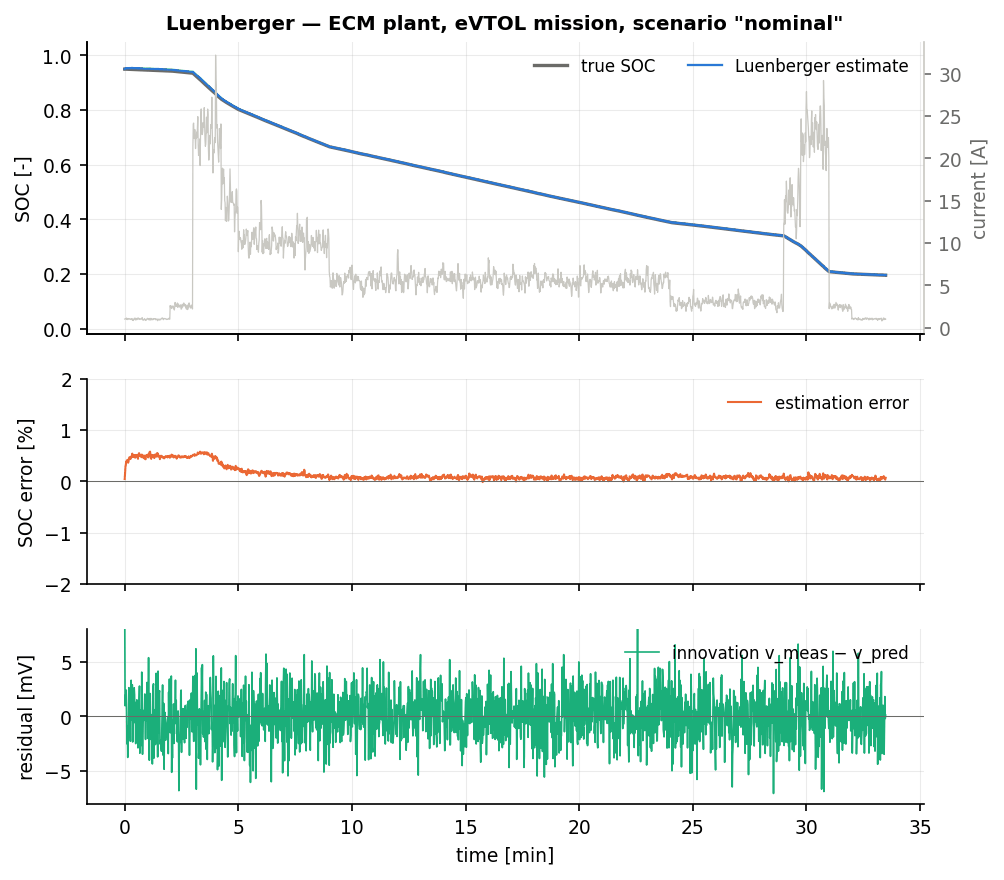
\includegraphics[width=\textwidth]{figures/cell_Luenberger_nominal.png}
\caption{Luenberger on the nominal eVTOL mission: true and estimated SOC (top), estimation error with the $\pm 2\sigma$ band when available (middle), voltage residual (bottom).}
\end{figure}
\begin{figure}[H]\centering
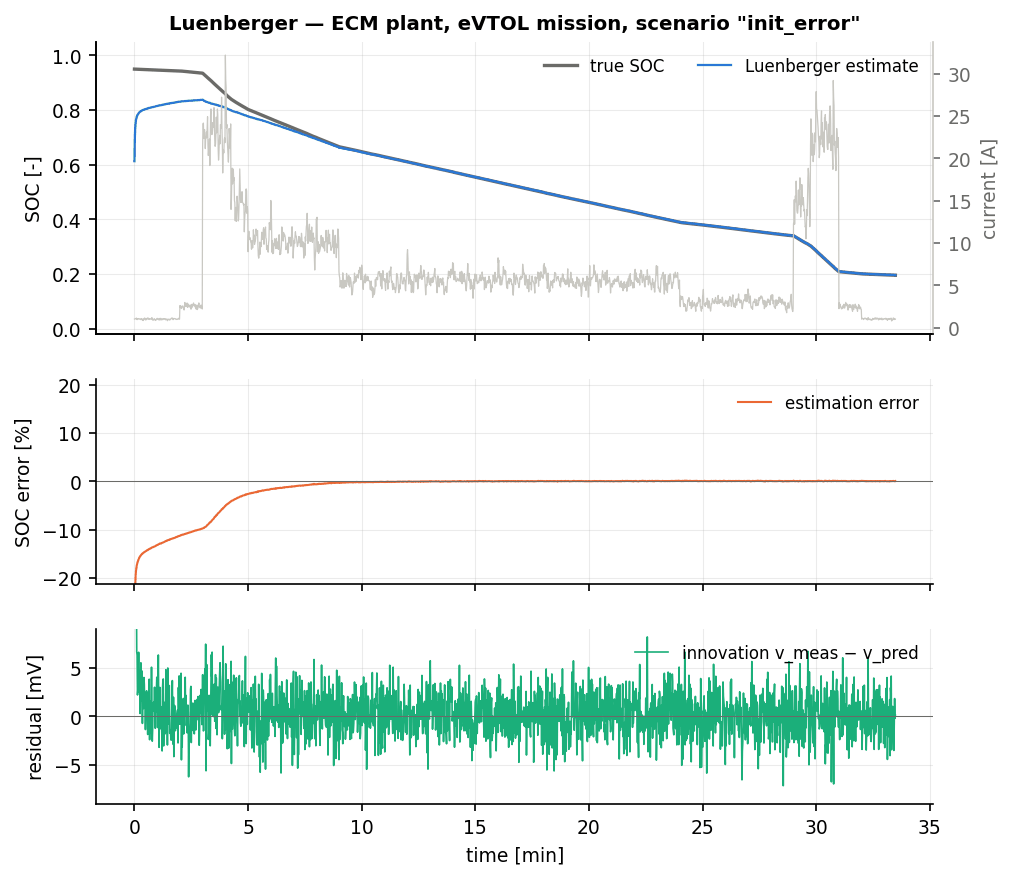
\includegraphics[width=\textwidth]{figures/cell_Luenberger_init_error.png}
\caption{Luenberger with a 35\,\% initial SOC error.}
\end{figure}

All numbers below are over three seeds; the spread is quoted whenever it is not negligible.  On
the nominal eVTOL mission the observer reaches $\mathrm{rmse}_{ss} = 0.0008$ SOC on every seed,
within a factor of two of the EKF's $0.0005$ and below the $0.02$ acceptance threshold by more
than an order of magnitude --- obtained without a covariance and at a third of the cost.  From a
$35\,\%$ initial error it converges in $334$\,s and settles to $0.0007$; the EKF converges faster
($0\,$s by the metric's definition) because its transient covariance gives it a large early gain,
which is precisely the advantage a fixed-gain observer gives up.

The scenario pattern follows the theory.  On \texttt{current\_bias} ($0.25$\,A offset plus a
$2\,\%$ gain error) the steady-state error is $0.0085$ against the EKF's $0.0061$: both are
dominated by \eqref{eq:lue-ssbias} with $\delta \approx R_0\Delta i \approx 4$\,mV, and no choice
of $\mL$ removes it.  On \texttt{param\_mismatch} ($R_0$ scaled by $0.7$) the observer gives
$0.0149$ versus the EKF's $0.0136$, and on \texttt{aged\_cell} $0.0218$ versus $0.0152$ --- again
the same mechanism.  \texttt{noise\_step} ($\sigma_v$ jumps to 20\,mV) barely moves the
Luenberger ($0.0033$) because a fixed gain cannot over-trust the measurement, whereas the
adaptive Kalman family has to detect the change first.  The most striking column is
\texttt{combined}, where the EKF reaches $\mathrm{rmse}_{ss}=0.1244$ and never converges, while
the Luenberger observer stays at $0.0213$ ($0.0204$--$0.0220$ across seeds) and converges in
$816$\,s: with four simultaneous faults the EKF's covariance is no longer a description of
anything, and a designed-bandwidth observer degrades far more gracefully than a mis-specified
optimal one.  The weakest columns are \texttt{aged\_cell} and \texttt{combined}, both limited by
\eqref{eq:lue-ssbias} rather than by the gain, and \texttt{preisach} ($0.0100$, where the
one-state hysteresis model is structurally wrong).

On the single-particle plant, where the estimator runs an ECM identified against a very different
model, the observer is at $0.0061$ on \texttt{nominal} and $0.0335$ on \texttt{cold} against the
EKF's $0.0373$ and $0.0735$ --- a factor of six and two respectively.  The ordering reverses
relative to the ECM plant for the same reason as \texttt{combined}: when the model is wrong the
optimal filter is optimal for the wrong problem.

\subsection*{How often is the placement actually used?}
The certification of \Cref{sec:lue-schedule} is not a formality.  Counting accepted placements
against total re-designs over the twelve ECM scenarios, the certified pole-placement gain is used
on $0/283$ re-designs on \texttt{nominal}, $0/331$ on \texttt{hot}, $0/420$ on
\texttt{param\_mismatch} and $0/445$ on \texttt{aged\_cell}, but $70$--$78$ of $\sim\!185$
($\approx 40\,\%$) on \texttt{cold} and $58$--$69$ of $\sim\!325$ ($\approx 20\,\%$) on
\texttt{combined}; the rest of the time the certified LQE gain is used instead.  The reason is
visible in the raw numbers: on \texttt{nominal} the placement gain achieves $\rho = 0.9986$ at the
frozen pair --- comfortably stable --- but $\rho = 1.0013$ to $1.0081$ over the family
\eqref{eq:lue-robust}, whereas the LQE gain achieves $0.9994$ to $0.9998$.  \emph{Exact
single-output pole placement is simply not robustly realisable on this plant at this sampling
rate}, and that is the honest headline of this chapter: the useful artefact is not the Ackermann
formula but the certification wrapper around it, which is what lets the same class carry a
placement design where one exists and an LQE design where one does not.  It also explains why
\texttt{Luenberger}, \texttt{HGO} and \texttt{SSKF} agree to three digits on most scenarios ---
they are running the same certified LQE gain --- and differ exactly on \texttt{cold}, where the
placement is admitted ($0.0040$ versus $0.0031$).

\section{Summary}
Use the Luenberger observer when the noise statistics are unknown or untrustworthy, when the
certification argument is about bounded convergence rather than optimality, or when the cycle
budget does not allow a covariance propagation.  Specify the poles as a repeated set, map them
from a time constant with $p=e^{-\dt/\tau}$, and validate every scheduled gain against a family
of perturbed linearisations rather than the frozen pair.  Do not use it when a calibrated
uncertainty output is required, when the measurement noise is genuinely non-stationary and you
want to exploit that, or when the dominant error is a persistent sensor bias --- for that,
continue to \Cref{ch:dob} or \Cref{ch:uio}.

% Copyright 2026 Sreeram Anil
% SPDX-License-Identifier: CC-BY-4.0
% =============================================================================
%  Steady-state Kalman filter / LQE observer
% =============================================================================
\chapter{Steady-State Kalman (LQE) Observer (SSKF)}
\label{ch:sskf}

\section*{At a glance}
\begin{tabular}{@{}l>{\raggedright\arraybackslash}p{0.76\textwidth}@{}}
Family & Deterministic observers \\
Header & \texttt{include/estkit/observers/luenberger.hpp} (\texttt{design = Riccati}) \\
Registered name & \texttt{SSKF} \\
State dimension & $n_x = 4$ (cell model) --- generic in $n_x, n_u, n_y$ \\
Cost per step & $\mathcal{O}(n_x^2)$ steady state; one DARE solve at reset; $\approx 0.5\,\mu$s/step measured \\
Primary references & \cite{kalman1960,andersonmoore1979,luenberger1971,simon2006} \\
\end{tabular}

\section{Motivation and aerospace/BMS relevance}
The Kalman filter's gain sequence $\mK_k$ converges, for a time-invariant detectable and
stabilisable pair, to a constant $\mK_\infty$ \cite[Sec.~4.4]{andersonmoore1979}.  Once it has
converged, propagating $\mP_k$ every sample buys nothing except the covariance output.  The
steady-state Kalman filter --- in the control literature, the \emph{linear quadratic estimator} --
throws the recursion away and keeps $\mK_\infty$.

This is the standard industrial compromise and it is everywhere in flight hardware: the
complementary filters in inertial systems, the fixed-gain attitude estimators of small UAVs, and
most shipping BMS SOC estimators are steady-state Kalman filters in disguise.  The reasons are
the same as for the Luenberger observer (\Cref{ch:luenberger}) --- bounded execution time, no
covariance to corrupt --- with one addition: the gain is not an arbitrary design choice but the
one that minimises the stationary error variance under the model's own $\mQ$ and $\mR$.  When a
BMS supplier can defend $\mQ$ and $\mR$ from sensor datasheets, that is a much easier
certification story than ``we chose $\tau = 60$\,s''.

The SSKF is registered from the same class as the Luenberger observer with
\texttt{design = Riccati}; the two registrations therefore isolate exactly one variable, the
origin of the gain, and the benchmark comparison between them is a controlled experiment.

\section{Problem statement and assumptions}
The plant is \eqref{eq:lue-plant-f}--\eqref{eq:lue-plant-h} with the additional assumption that
$\vw_k$ and $\vv_k$ are zero-mean, mutually uncorrelated white sequences with
\begin{equation}
\E{\vw_k\vw_k^\T} = \mQ(\vx,\vu), \qquad \E{\vv_k\vv_k^\T} = \mR(\vx,\vu) ,
\label{eq:sskf-noise}
\end{equation}
both supplied by the model.  We additionally require $(\mA,\mC)$ detectable and
$(\mA,\mQ^{1/2})$ stabilisable, which guarantee a unique stabilising solution of the discrete
algebraic Riccati equation.

\section{Derivation}

\subsection{The algebraic Riccati equation}
Let $\Pminus_k = \E{(\xminus_k-\vx_k)(\xminus_k-\vx_k)^\T}$.  The Kalman recursion in
current-estimator form is
\begin{align}
\mS_k &= \mC\Pminus_k\mC^\T + \mR , \label{eq:sskf-S}\\
\mK_k &= \Pminus_k\mC^\T\mS_k\inv , \label{eq:sskf-K}\\
\Pminus_{k+1} &= \mA\big(\Pminus_k - \mK_k\mC\Pminus_k\big)\mA^\T + \mQ . \label{eq:sskf-riccati}
\end{align}
For a time-invariant detectable/stabilisable pair the map \eqref{eq:sskf-riccati} has a unique
positive semi-definite fixed point $\mP_\infty$ and $\Pminus_k\to\mP_\infty$ from any
$\Pminus_0\succeq 0$ \cite[Thm.~4.1]{andersonmoore1979}.  The steady-state gain is
\begin{equation}
\mK_\infty = \mP_\infty\mC^\T\big(\mC\mP_\infty\mC^\T+\mR\big)\inv ,
\label{eq:sskf-Kinf}
\end{equation}
and the observer is \eqref{eq:lue-predict}--\eqref{eq:lue-update} with $\mL = \mK_\infty$.  Note
that $\mP_\infty$ in \eqref{eq:sskf-riccati} is the \emph{prior} covariance, which is why
$\mK_\infty$ is directly the current-estimator gain and no conversion \eqref{eq:lue-Lconv} is
needed.

\subsection{Optimality and its limits}
$\mK_\infty$ minimises $\tr \mP^+$ in the stationary regime, so among all constant gains it is
the minimum-variance choice \emph{for the assumed $\mQ,\mR$}.  Two consequences matter here.

First, the transient is sacrificed.  The time-varying filter starts with $\Pminus_0 = \mP_0$,
which for the benchmark is $\sigma_{z0}=0.1$ on the SOC channel, four orders of magnitude above
the stationary $\mP_{\infty,11}$; its early gain is therefore much larger and it recovers from an
initial error far faster.  The steady-state filter has the small gain from the first sample.
This is visible in the benchmark as $334$\,s convergence on \texttt{init\_error} against the
EKF's $0$\,s.

Second, the bandwidth is set entirely by the ratio $\mQ/\mR$.  For a scalar random walk observed
in noise, the fixed point of \eqref{eq:sskf-riccati} satisfies $P^2 = QP + QR$, so for $Q\ll R$,
$P\approx\sqrt{QR}$ and
\begin{equation}
K \approx \frac{c\sqrt{QR}}{c^2\sqrt{QR}+R} \approx \frac{1}{c}\sqrt{\frac{Q}{R}} ,\qquad
1 - Kc \approx 1 - \sqrt{Q/R} ,
\label{eq:sskf-scalar}
\end{equation}
i.e. the closed-loop time constant is $\tau \approx \dt\sqrt{R/Q}$.  The SOC bandwidth is
therefore a statement about how much unmodelled SOC drift one admits per sample, and nothing
else.  With the cell model's own floor $q_{\soc}=10^{-5}$ and
$R = \sigma_v^2 + (R_0\sigma_i)^2 = 4.4\times10^{-6}$, \eqref{eq:sskf-scalar} gives
$\tau\approx1300$\,s --- longer than the whole eVTOL mission.

\subsection{Choosing the process-noise allowance}
\label{sec:sskf-q}
The fix is not a tuning trick; it is the recognition that the SOC channel carries a real,
unmodelled drift.  Over a mission of $N$ samples a per-step standard deviation $q_{\soc}$
accumulates to $q_{\soc}\sqrt{N}$ of SOC.  For $N = 20\,010$ samples:
\begin{center}
\begin{tabular}{@{}lll@{}}
\toprule
$q_{\soc}$ per step & accumulated SOC drift & physical equivalent \\
\midrule
$10^{-5}$ (model floor) & $0.14\,\%$ & coulomb counter with a perfect sensor \\
$10^{-4}$ (used here)   & $1.4\,\%$  & $\approx 0.12$\,A of current-sensor bias on a 5\,Ah cell \\
$10^{-3}$               & $14\,\%$   & gross capacity error \\
\bottomrule
\end{tabular}
\end{center}
The benchmark's \texttt{current\_bias} scenario has a $0.25$\,A offset, i.e. $2.8\,\%$ SOC of
drift, so $q_{\soc}=10^{-4}$ is a defensible design value rather than a fitted one, and it is
what \texttt{Options::q\_extra[IZ]} is set to.  With it, \eqref{eq:sskf-scalar} gives
$\tau\approx 130$\,s and the measured \texttt{init\_error} convergence is $334$\,s.

\subsection{Solving the DARE without an eigen-solver}
The obvious method is to iterate \eqref{eq:sskf-riccati} as a fixed point
(\texttt{dare\_iterate}), which converges linearly at rate $\rho\big((\mI-\mK\mC)\mA\big)^2$.  For
this plant that rate is $\approx 0.9994$ per sweep, so a truncated run does not return a slightly
detuned gain: it returns the finite-horizon Kalman gain of a filter that has only run for
$n_{\mathrm{iter}}$ samples.  At the library's default of $4000$ sweeps that gain has the
\emph{wrong sign} on the SOC channel ($L_{\soc}=-0.61$ against the converged $+0.066$), and an
observer built on it diverges.  Reaching the steady state this way needs $\mathcal{O}(10^4)$
sweeps.

The observers of this family therefore use the structure-preserving doubling algorithm
(\texttt{dare\_doubling}) for the initial solve, one per \texttt{reset()}.  Each doubling step
squares the closed-loop propagator, so the effective horizon doubles and $60$--$80$ iterations
reach the stabilising solution to machine precision.  Whenever the linearisation subsequently
moves, $40$ warm-started plain sweeps from the stored $\mP$ are enough, because the solution
moves only slightly.  That is the practical reason the class keeps $\mP$ at all: not to report
uncertainty, but to warm-start the re-design.  \texttt{Options::riccati\_exact = false} selects
the truncated recursion for the rare case where a deliberately soft start-up gain is wanted.

\section{Algorithm}
\begin{algorithm}[H]
\caption{SSKF --- design (at reset) and one sampling period}
\begin{algorithmic}[1]
\Statex \textbf{Design (once, at the first measurement update):}
\State $\mQ_d \gets q_s\mQ(\xhat,\vu) + \diag(\bm{q}_{\mathrm{extra}}^2)$, \quad $\mR_d \gets r_s\mR(\xhat,\vu)$
\State Solve \eqref{eq:sskf-riccati} by doubling; \quad $\mL \gets \mP\mC^\T(\mC\mP\mC^\T+\mR_d)\inv$
\Statex \textbf{Each sample:}
\State $\xminus_k \gets f(\xplus_{k-1},\vu_{k-1})$; \quad $\yhat_k \gets h(\xminus_k,\vu_k)$
\If{the linearisation has moved by more than $\delta_{\mathrm{tol}}$}
  \State warm-start \eqref{eq:sskf-riccati} from the stored $\mP$ for $n_{\mathrm{refine}}$ iterations; update $\mL$ if it passes the robust check \eqref{eq:lue-robust}
\EndIf
\State $\xplus_k \gets \xminus_k + \mL\,(\vy_k - \yhat_k)$; \quad $\xplus_k \gets \operatorname{constrain}(\xplus_k)$
\Ensure $\xplus_k$
\end{algorithmic}
\end{algorithm}

\section{Application to the battery model}
$\mQ$ and $\mR$ come from the model and are themselves scheduled: the cell model builds
$\mQ = \bm{b}\bm{b}^\T\sigma_i^2 + \diag(\bm{q}_{\mathrm{floor}}^2)$ with
$\bm{b} = \partial f/\partial i$, i.e. the process noise is the current-sensor noise mapped
through the input Jacobian, and $\mR = \sigma_v^2 + (R_0(T)\sigma_i)^2$ adds the ohmic
contribution of the same current noise to the voltage measurement.  Because $\bm{b}$ and $R_0$
depend on $T$ and on the operating point, the steady-state gain is re-computed by warm start
whenever the linearisation moves, which makes this a genuinely gain-scheduled LQE and not a
single constant matrix.

Measured gain at $25^\circ$C, $\soc = 0.9$, $q_{\soc}=10^{-4}$:
$\mL = [5.4\times10^{-2},\,-1.3\times10^{-2},\,-2.1\times10^{-2},\,-0.76]^\T$.  The signs are
informative: a positive residual (measured voltage above prediction) raises $\soc$ and lowers
both RC over-potentials, which is exactly the physical interpretation of ``the cell is fuller
than I thought, or I have over-estimated the polarisation''.

\section{Implementation notes}
Identical object and per-step path to \Cref{ch:luenberger} --- the difference is entirely in
where $\mL$ comes from, so the two registrations share $4624$ bytes and the same update code.
The extra cost is the DARE solve at reset ($60$--$80$ doubling steps on a $4\times4$ system,
well under a millisecond), which appears in the benchmark's $0.5\,\mu$s/step figure because
\texttt{reset()} is inside the timed region; the steady-state per-step cost is the same
$\approx 0.2\,\mu$s as the Luenberger observer.  On an embedded target one would solve the DARE
offline on a grid of $(T,\soc)$ and interpolate, which is standard BMS practice and removes the
start-up cost entirely.

The class deliberately does not expose \texttt{P()}: $\mP_\infty$ is the covariance of the
\emph{assumed} model, and reporting it as an uncertainty would be misleading in exactly the
scenarios (bias, mismatch, ageing) where the assumption fails.

\section{Benchmark results}
\input{tables/cell_SSKF.tex}
\begin{figure}[H]\centering
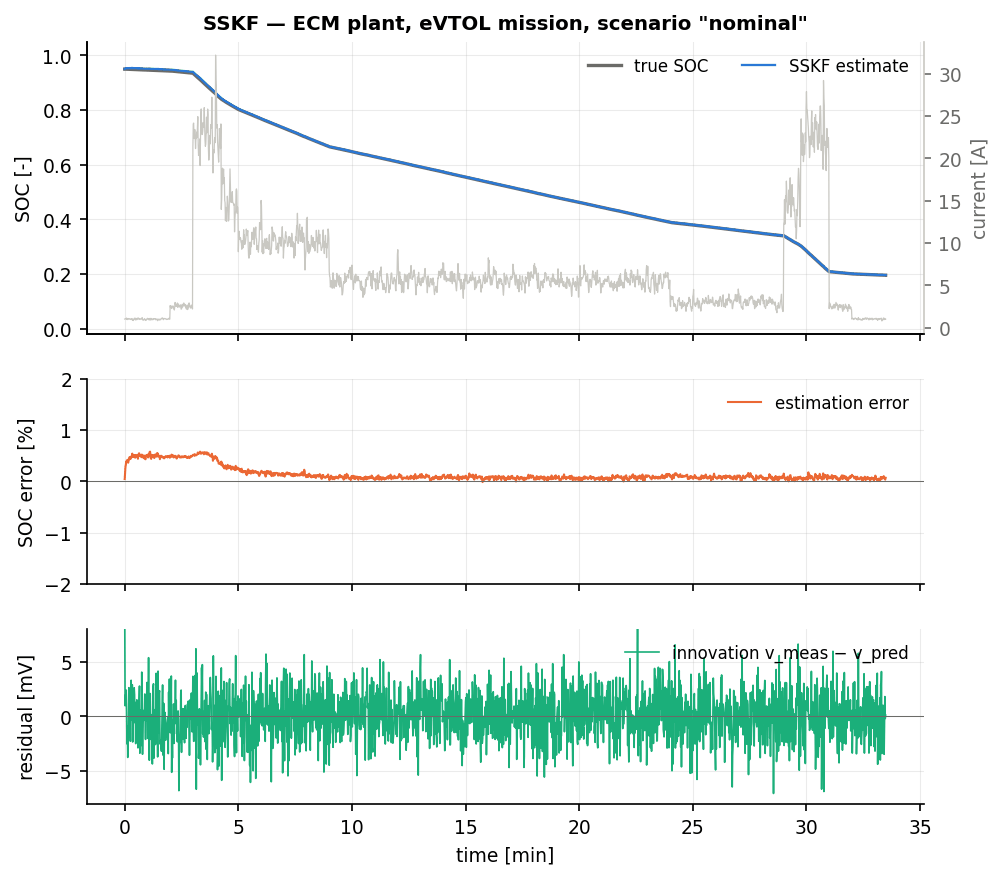
\includegraphics[width=\textwidth]{figures/cell_SSKF_nominal.png}
\caption{SSKF on the nominal eVTOL mission: true and estimated SOC (top), estimation error with the $\pm 2\sigma$ band when available (middle), voltage residual (bottom).}
\end{figure}
\begin{figure}[H]\centering
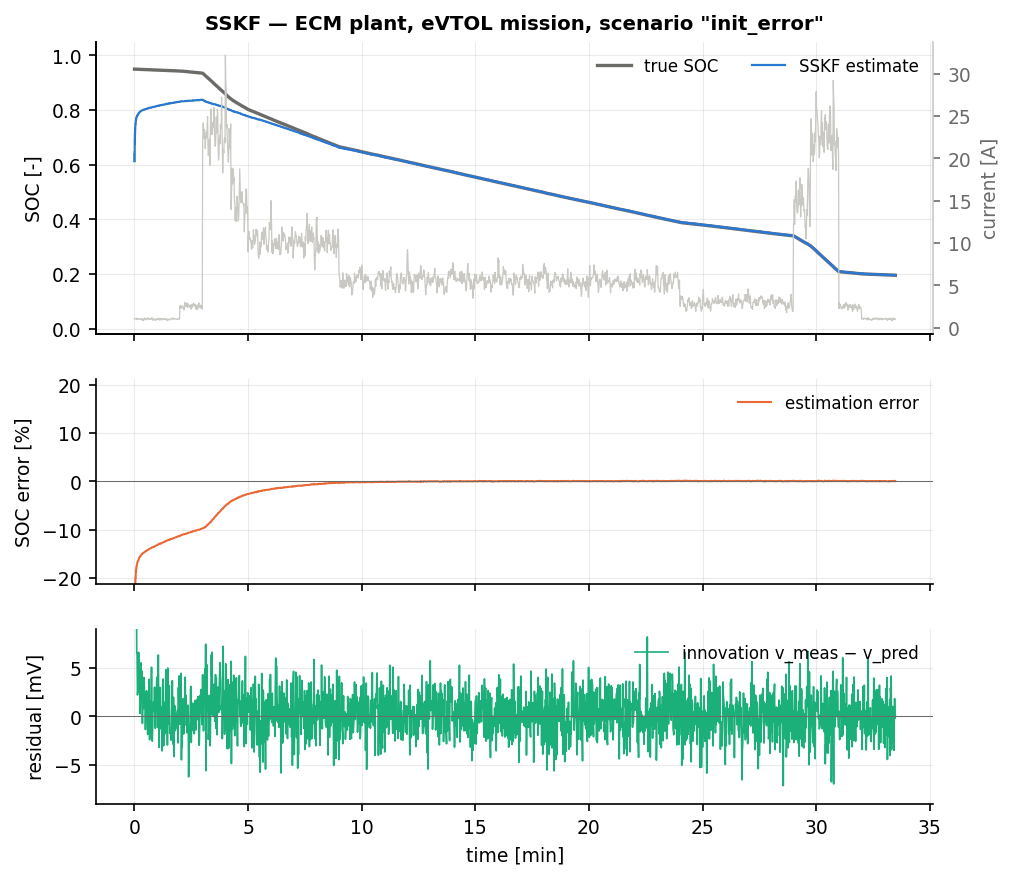
\includegraphics[width=\textwidth]{figures/cell_SSKF_init_error.png}
\caption{SSKF with a 35\,\% initial SOC error.}
\end{figure}

All numbers are over three seeds.  The SSKF reaches $\mathrm{rmse}_{ss}=0.0008$ on
\texttt{nominal} on every seed --- the lowest voltage-residual RMS of the whole observer family
and within a factor of two of the EKF's $0.0005$.  That is the expected result: with the correct
model and the correct noise description, the constant gain is as good as the recursive one in
steady state.  The cost is the transient.  On \texttt{init\_error} the SSKF needs $334$\,s
against the EKF's $0$\,s, because its gain is the stationary one from the first sample; the final
accuracy is then identical ($0.0007$).  This single comparison is the clearest statement of what
the covariance recursion actually buys: nothing in steady state, everything in the transient.

The exact solution of \eqref{eq:lue-dare} matters here more than anywhere else in the family,
because the SSKF \emph{is} that solution.  Iterating the recursion converges linearly at rate
$\rho((\mI-\mK\mC)\mA)^2 \approx 0.9994$ per sweep, so truncating it at a few thousand sweeps does
not give a slightly detuned gain --- it gives the finite-horizon gain of a filter that has only
run for a few thousand samples, and for this plant that gain has the wrong \emph{sign} on the SOC
channel ($L_z=-0.61$ against the converged $+0.066$).  The doubling algorithm removes the question
entirely at $60$--$80$ iterations.

Across the fault scenarios the SSKF tracks the pole-placed observer closely --- to three digits
on most of them, because the certification of \Cref{sec:lue-schedule} rejects the placement on
those scenarios and both registrations then run the same LQE gain (\Cref{ch:luenberger}).  Where
the placement \emph{is} admitted the SSKF is better: \texttt{cold} $0.0031$ against the
Luenberger's $0.0040$, because the LQE design automatically re-weights when the RC time constants
stretch, whereas a fixed pole set asks for the same bandwidth at $-10^\circ$C as at
$25^\circ$C.  \texttt{current\_bias} ($0.0085$), \texttt{aged\_cell} ($0.0218$) and
\texttt{param\_mismatch} ($0.0149$) are all limited by \eqref{eq:lue-ssbias}: the residual bias
is a property of the model error and the OCV slope, not of the gain.  On \texttt{combined} the
SSKF ends at $0.0203$ ($0.0202$--$0.0205$ across seeds) against the EKF's $0.1244$ and no
convergence --- again, a fixed sensible gain degrades far better than a mis-specified optimal one
--- and on the single-particle plant it is at $0.0061$ on \texttt{nominal} and $0.0335$ on
\texttt{cold} against the EKF's $0.0373$ and $0.0735$.

\section{Summary}
Take the SSKF when $\mQ$ and $\mR$ are defensible and the start-up transient is not critical: it
gives EKF-quality steady-state accuracy at a third of the run-time cost and with no covariance
to go indefinite.  Add an explicit process-noise allowance on any integrating channel, because
the model's noise floor there is usually a numerical guard rather than a physical statement.
Avoid it when the measurement noise is strongly non-stationary, when a fast recovery from a bad
initial condition matters, or when a calibrated uncertainty output is required.

% Copyright 2026 Sreeram Anil
% SPDX-License-Identifier: CC-BY-4.0
% =============================================================================
%  Proportional-integral observer
% =============================================================================
\chapter{Proportional-Integral Observer (PI-Observer)}
\label{ch:piobserver}

\section*{At a glance}
\begin{tabular}{@{}l>{\raggedright\arraybackslash}p{0.76\textwidth}@{}}
Family & Deterministic observers \\
Header & \texttt{include/estkit/observers/pi\_observer.hpp} \\
Registered name & \texttt{PI-Observer} \\
State dimension & $n_x + n_y = 5$ (cell model) --- generic in $n_x, n_u, n_y$ \\
Cost per step & $\mathcal{O}((n_x{+}n_y)^2)$ steady state; $\approx 1.3\,\mu$s/step measured \\
Primary references & \cite{wojciechowski1978,beale1989pi,shafai1996ltrpi,johnson1971dac,luenberger1971} \\
\end{tabular}

\section{Motivation and aerospace/BMS relevance}
A proportional observer drives the output residual towards zero but leaves a steady-state state
error whenever the \emph{state} equation is corrupted by a constant disturbance.  This is the
observer analogue of the offset that a pure P controller leaves, and the cure is the same:
integral action.  Wojciechowski \cite{wojciechowski1978} introduced the proportional-integral
observer for exactly this reason, and Beale and Shafai \cite{beale1989pi} showed that the extra
integral gain also buys robustness margins that a proportional observer cannot achieve, because
the additional design freedom can be used to shape the loop rather than only to place poles.
Shafai et al.\ \cite{shafai1996ltrpi} later gave the discrete-time loop-transfer-recovery
version.

For a battery this matters because the SOC channel is a pure integrator fed by a measured
current.  Anything that corrupts that current --- a sensor offset, a coulombic-efficiency error,
a capacity that has faded since the last calibration --- appears as a constant (or slowly
varying) disturbance on $\dot{\soc}$, precisely the case integral action is designed for.  In an
eVTOL application the consequence of a slow SOC drift is a mis-stated reserve at the end of the
mission, which is a flight-safety quantity, so a structure that provably removes a constant
$\dot{\soc}$ offset is worth its extra state.

\section{Problem statement and assumptions}
Plant \eqref{eq:lue-plant-f}--\eqref{eq:lue-plant-h} augmented with an unknown constant state
disturbance $\bm{d}\in\real^{n_y}$ entering through a distribution matrix
$\mG\in\real^{n_x\times n_y}$:
\begin{equation}
\vx_{k+1} = f(\vx_k,\vu_k) + \mG\bm{d}_k , \qquad \bm{d}_{k+1} = \bm{d}_k , \qquad
\vy_k = h(\vx_k,\vu_k) + \vv_k .
\label{eq:pi-plant}
\end{equation}
\begin{assumption}[Augmented observability]\label{as:pi-obs}
$(\mA,\mC)$ is observable and the augmented pair is observable, which by the
Popov--Belevitch--Hautus test at $z=1$ requires
\begin{equation}
\operatorname{rank}\begin{bmatrix}\mA-\mI & \mG\\ \mC & \bm{0}\end{bmatrix} = n_x + n_y ,
\label{eq:pi-hautus}
\end{equation}
i.e. the triple $(\mA,\mG,\mC)$ has no transmission zero at $z=1$.
\end{assumption}

\section{Derivation}

\subsection{The PI structure and its equivalent augmented observer}
The PI observer of \cite{wojciechowski1978,beale1989pi} adds an integral of the output error to
the correction,
\begin{align}
\bm{\xi}_{k+1} &= \bm{\xi}_k + \big(\vy_k - \yhat_k\big) , \label{eq:pi-xi}\\
\xplus_k &= \xminus_k + \mL_P\big(\vy_k-\yhat_k\big) + \mL_I\bm{\xi}_k .\label{eq:pi-update}
\end{align}
Written like this, the design problem is a \emph{structured} output-injection problem and
Ackermann's formula does not apply.  The implementation therefore uses the equivalent, and
classical, formulation as a Luenberger observer of the augmented plant \eqref{eq:pi-plant}:
\begin{align}
\xminus_k &= f(\xplus_{k-1},\vu_{k-1}) + \mG\,\hat{\bm{d}}^+_{k-1} , &
\hat{\bm{d}}^-_k &= \hat{\bm{d}}^+_{k-1} , \label{eq:pi-pred}\\
\bm{r}_k &= \vy_k - h(\xminus_k,\vu_k) , & & \label{eq:pi-res}\\
\xplus_k &= \xminus_k + \mL_P\bm{r}_k , &
\hat{\bm{d}}^+_k &= \hat{\bm{d}}^-_k + \mL_I\bm{r}_k . \label{eq:pi-upd}
\end{align}
Unrolling the second line of \eqref{eq:pi-upd} gives
$\hat{\bm{d}}^+_k = \sum_{j\le k}\mL_I\bm{r}_j$, so $\hat{\bm{d}}$ \emph{is} the integral state
$\bm{\xi}$ up to the factor $\mL_I$, and $\mG\hat{\bm{d}}$ is the integral correction of
\eqref{eq:pi-update}.  The two formulations are identical; the second is a standard pole
assignment on
\begin{equation}
\bar{\mA} = \begin{bmatrix}\mA & \mG\\ \bm{0} & \mI\end{bmatrix}\in\real^{(n_x+n_y)\times(n_x+n_y)} ,
\qquad
\bar{\mC} = \begin{bmatrix}\mC & \bm{0}\end{bmatrix} ,
\label{eq:pi-aug}
\end{equation}
which for $n_y = 1$ is a single-output problem and yields to Ackermann's formula.

\subsection{Error dynamics and steady-state rejection}
With $\bm{\eta}_k = [(\xplus_k-\vx_k)^\T\ (\hat{\bm{d}}^+_k-\bm{d})^\T]^\T$ and
$\bar{\mL} = [\mL_P^\T\ \mL_I^\T]^\T$,
\begin{equation}
\bm{\eta}_k = \big(\mI - \bar{\mL}\bar{\mC}\big)\bar{\mA}\,\bm{\eta}_{k-1}
            - \bar{\mL}\vv_k + \mathcal{O}(\norm{\bm{\eta}_{k-1}}^2) .
\label{eq:pi-err}
\end{equation}
Under \Cref{as:pi-obs} the $n_x+n_y$ poles can be placed anywhere inside the unit disc; the
design then guarantees
\begin{equation}
\lim_{k\to\infty}\xplus_k - \vx_k = \bm{0}
\qquad\text{for any constant }\bm{d},
\label{eq:pi-zero}
\end{equation}
which is the property a proportional observer does not have.  The conversion to
current-estimator form is $\bar{\mL} = \bar{\mA}\inv\bar{\mL}_{\mathrm{pred}}$ exactly as in
\eqref{eq:lue-Lconv}, with $\bar{\mA}$ invertible whenever $\mA$ is.

\subsection{Choosing the disturbance direction}
\label{sec:pi-G}
$\mG$ encodes \emph{where} the constant disturbance is believed to act.  When no physical model
is available the implementation picks it automatically and model-agnostically as the unit vector
of the state with the largest DC gain from a constant disturbance:
\begin{equation}
j^\star = \arg\max_j \ \norm{(\mI-\mA+\mu\mI)\inv \bm{e}_j}_1 ,
\qquad \mG = \bm{e}_{j^\star} ,
\label{eq:pi-Gauto}
\end{equation}
with a small regularisation $\mu$ so that an exact integrator does not produce a singular
matrix.  The interpretation is direct: put the integral action on the state that cannot correct
itself.  For the cell model $\mA = \diag(1,a_1,a_2,a_h)$ and \eqref{eq:pi-Gauto} returns the SOC
integrator, so the integral action lands exactly where coulomb-counting drift accumulates.

\subsection{Pole selection and anti-windup}
Two time scales are specified: the $n_x$ plant-mode poles (\texttt{Options::pole}, a repeated
set as argued in \Cref{sec:lue-spread}) and the $n_y$ integral poles
(\texttt{Options::pole\_i}).  Making the integral loop slower than the state loop is the usual
rule; with $\tau_x = 40$\,s and $\tau_i = 100$\,s the measured steady-state SOC standard
deviation is $2.8\times10^{-3}$ and the linear error decay from a $0.35$ initial offset reaches
$5\times10^{-3}$ within 300\,s.

An integrator needs anti-windup.  \texttt{Options::d\_max} bounds $\norm{\hat{\bm{d}}}_\infty$;
for the cell it is set to $6\times10^{-5}$ SOC per step, i.e. the drift a $10$\,A current-sensor
error would produce.  The bound turns out to be \emph{two-sided} in its effect, and both sides
were measured:
\begin{itemize}[nosep]
\item too large, and the integrator absorbs an error that is not a state disturbance at all.  On
the \texttt{cold} scenario the Arrhenius law raises $R_0$ by $\approx 90\,\%$, which is an
\emph{output}-map error; \Cref{sec:pi-limits} shows integral action cannot remove it, so the
integrator merely chases it and drags the SOC estimate with it.
\item too small, and the integrator can no longer absorb the disturbances that \emph{are} state
disturbances.  Sweeping $d_{\max}$ over three seeds, $\mathrm{rmse}_{ss}$ on \texttt{cold} goes
$0.0107$ at $6\times10^{-5}$, $0.0214$ at $3\times10^{-5}$, $0.0293$ at $3\times10^{-6}$ and
$0.359$ at $10^{-6}$; on \texttt{combined} it goes $0.021$, $0.020$, $0.354$, $0.429$.  The
collapse below $10^{-5}$ is not windup --- it is the opposite, an integrator clamped so hard that
the real $10\,\%$ capacity loss and $0.15$\,A bias have nowhere to go but the SOC estimate.
\end{itemize}
$6\times10^{-5}$ is the measured optimum over the twelve scenarios.

The gain \emph{certification} of \Cref{sec:lue-schedule} applies unchanged to the augmented
pair, and matters more here than anywhere else: $\det\bar{\mathcal{O}}\approx 7\times10^{-26}$
for the cell, so the shift-and-scale of \eqref{eq:lue-shift} is what makes the design computable
at all, and the certified decay margin is what makes it safe.  Before certification was applied
to the augmented placement this observer diverged on two seeds out of three on \texttt{cold}
($\mathrm{rmse}_{ss}=0.42$), while the third seed was at $0.004$ --- a textbook illustration of
why a single-seed benchmark is not evidence of robustness.

\section{Algorithm}
\begin{algorithm}[H]
\caption{PI-Observer --- one sampling period}
\begin{algorithmic}[1]
\Require $\xplus_{k-1}$, $\hat{\bm{d}}^+_{k-1}$, $\vu_{k-1}$, $\vy_k$, $\vu_k$, gains $\mL_P,\mL_I$
\State \textbf{Time update:} $\xminus_k \gets f(\xplus_{k-1},\vu_{k-1}) + \mG\hat{\bm{d}}^+_{k-1}$, \quad $\hat{\bm{d}}^-_k \gets \hat{\bm{d}}^+_{k-1}$
\State \textbf{Prior output:} $\yhat_k \gets h(\xminus_k,\vu_k)$
\If{the linearisation has moved by more than $\delta_{\mathrm{tol}}$}
  \State build $\mG$ from \eqref{eq:pi-Gauto} and $(\bar{\mA},\bar{\mC})$ from \eqref{eq:pi-aug}
  \State assign $\{p_1..p_{n_x}\}\cup\{p_{I,1}..p_{I,n_y}\}$ by shifted-scaled Ackermann; convert with $\bar{\mA}\inv$
  \State accept only if $\norm{\bar{\mL}}_\infty \le L_{\max}$ and the robust check \eqref{eq:lue-robust} passes
\EndIf
\State $\bm{r}_k \gets \vy_k - \yhat_k$; \quad $\bm{\xi}_k \gets \bm{\xi}_{k-1} + \bm{r}_k$
\State $\xplus_k \gets \xminus_k + \mL_P\bm{r}_k$; \quad $\hat{\bm{d}}^+_k \gets \operatorname{sat}\big(\hat{\bm{d}}^-_k + \mL_I\bm{r}_k;\ d_{\max}\big)$
\State $\xplus_k \gets \operatorname{constrain}(\xplus_k)$
\Ensure $\xplus_k$, $\hat{\bm{d}}^+_k$
\end{algorithmic}
\end{algorithm}

\section{Application to the battery model}
With $\mG = \bm{e}_{\soc}$ the augmented pair is
\begin{equation}
\bar{\mA} = \begin{bmatrix}1&0&0&0&1\\0&a_1&0&0&0\\0&0&a_2&0&0\\0&0&0&a_h&0\\0&0&0&0&1\end{bmatrix},
\qquad
\bar{\mC} = \big[\ \partial\ocv/\partial\soc\ \ {-1}\ \ {-1}\ \ M\ \ 0\ \big] ,
\label{eq:pi-cell}
\end{equation}
and the Hautus condition \eqref{eq:pi-hautus} holds because $a_1,a_2,a_h\neq 1$ and
$\partial\ocv/\partial\soc\neq 0$.  Note the \emph{two} unit eigenvalues of $\bar{\mA}$ (the SOC
integrator and the disturbance): they are distinguishable only through the dynamics, which is
why the augmented observability matrix is so ill-conditioned and why the integral pole must be
slower than the state poles.

Benchmark options: $\tau_x = 40$\,s (repeated), $\tau_i = 100$\,s, $L_{\max}=0.3$,
$d_{\max}=6\times10^{-5}$.

\subsection{What integral action can and cannot remove}
\label{sec:pi-limits}
It is worth being precise, because the benchmark result is counter-intuitive.  Integral action
drives $\bm{r}_k\to\bm{0}$ \emph{exactly}.  If the model error is a disturbance on the state
equation in the direction $\mG$, that is the same as $\bm{\eta}\to\bm{0}$ and the SOC error
vanishes.  But if the model error appears \emph{in the output map} --- say the predicted voltage
carries a bias $\delta$ because $R_0$ or the measured current is wrong --- then $\bm{r}\to\bm{0}$
forces $\mC\veps = \delta$, and with the non-integrating modes at zero this is again
\eqref{eq:lue-ssbias}:
\begin{equation}
\veps_{\soc}^{\,\infty} = \frac{\delta}{\partial\ocv/\partial\soc} ,
\label{eq:pi-ssbias}
\end{equation}
unchanged from the proportional observer.  A PI observer whose disturbance enters only the state
equation cannot remove an output-path bias.  For the current-sensor fault the dominant symptom
is exactly such a bias, through the ohmic drop $R_0\Delta i$, and the correct structures are
those of \Cref{ch:dob,ch:uio}, which feed the disturbance estimate back into $h$ as well as $f$.

\section{Implementation notes}
$4808$ bytes, no heap.  The extra cost over the Luenberger observer is one extra state, a
$5\times5$ instead of $4\times4$ design, and the Riccati fall-back at start-up; the measured
$1.3\,\mu$s/step is dominated by that one-off DARE solve inside the timed \texttt{reset()}, the
steady-state path being $\approx 250$\,ns.  Numerical points specific to this observer: the
augmented observability matrix is a Vandermonde-like matrix with two coincident nodes at $z=1$,
so the shift-and-scale of \Cref{sec:lue-cond} is mandatory; the disturbance integrator is
saturated; and a rejected re-design keeps the previous gain rather than switching to a
structurally different LQE gain, because swapping between two different loop shapes with a
non-zero integral state stored is itself a source of transients.

\section{Benchmark results}
% Copyright 2026 Sreeram Anil
% SPDX-License-Identifier: CC-BY-4.0
\begin{table}[H]\centering\footnotesize\setlength{\tabcolsep}{4pt}
\caption{PI-Observer: cell-level benchmark on the eVTOL mission (mean over seeds; RMSE and max error in \% SOC; $t_\mathrm{conv}$: first time the error stays below 2\,\% for 60\,s, -- = never; EKF reference: steady-state RMSE of the plain EKF on the same data).}\label{tab:cell_PIObserver}
\begin{tabular}{llrrrrrcrr}\toprule
plant & scenario & RMSE & RMSE$_\mathrm{ss}$ & max & $t_\mathrm{conv}$ [s] & RMSE$_v$ [mV] & div. & EKF ref. & ns/step \\ \midrule
ECM & nominal & 0.26 & 0.11 & 1.25 & 0 & 1.05 & no & 0.05 & 1373 \\
ECM & init\_error & 1.48 & 0.11 & 33.07 & 93 & 5.52 & no & 0.05 & 1455 \\
ECM & current\_bias & 1.27 & 0.99 & 5.24 & 0 & 0.92 & no & 0.61 & 1324 \\
ECM & noise\_step & 0.47 & 0.51 & 1.84 & 0 & 5.15 & no & 0.12 & 6958 \\
ECM & outliers & 0.34 & 0.37 & 1.35 & 0 & 3.20 & no & 0.21 & 2929 \\
ECM & cold & 0.83 & 0.77 & 2.79 & 0 & 3.62 & no & 0.16 & 699 \\
ECM & hot & 0.20 & 0.05 & 0.86 & 0 & 0.58 & no & 0.03 & 1357 \\
ECM & aged\_cell & 3.31 & 2.63 & 13.77 & 0 & 6.13 & no & 1.52 & 1619 \\
ECM & param\_mismatch & 2.00 & 1.59 & 9.08 & 0 & 3.27 & no & 1.36 & 1593 \\
ECM & sensor\_dropout & 0.57 & 0.11 & 6.26 & 0 & 1.90 & no & 0.46 & 1422 \\
ECM & preisach & 1.23 & 1.08 & 3.74 & 223 & 0.91 & no & 0.20 & 1286 \\
ECM & combined & 2.60 & 1.98 & 24.01 & 22 & 12.04 & no & 12.44 & 856 \\
\midrule
SPM & nominal & 1.09 & 0.97 & 4.91 & 0 & 1.07 & no & 3.73 & 1154 \\
SPM & init\_error & 1.46 & 0.97 & 32.88 & 26 & 4.92 & no & 3.81 & 1262 \\
SPM & current\_bias & 1.36 & 1.45 & 5.66 & 0 & 1.15 & no & 5.69 & 1302 \\
SPM & noise\_step & 1.55 & 1.79 & 4.91 & 0 & 3.44 & no & 3.30 & 7282 \\
SPM & outliers & 1.10 & 1.02 & 5.25 & 0 & 2.44 & no & 1.99 & 2937 \\
SPM & cold & 4.45 & 5.28 & 15.45 & 345 & 4.51 & no & 7.35 & 1521 \\
SPM & hot & 0.98 & 0.81 & 5.54 & 0 & 0.73 & no & 2.16 & 1249 \\
SPM & param\_mismatch & 2.42 & 1.33 & 9.17 & 0 & 2.00 & no & 3.13 & 1065 \\
SPM & sensor\_dropout & 1.14 & 0.99 & 7.79 & 0 & 2.00 & no & 5.31 & 1128 \\
\bottomrule\end{tabular}\end{table}

\begin{figure}[H]\centering
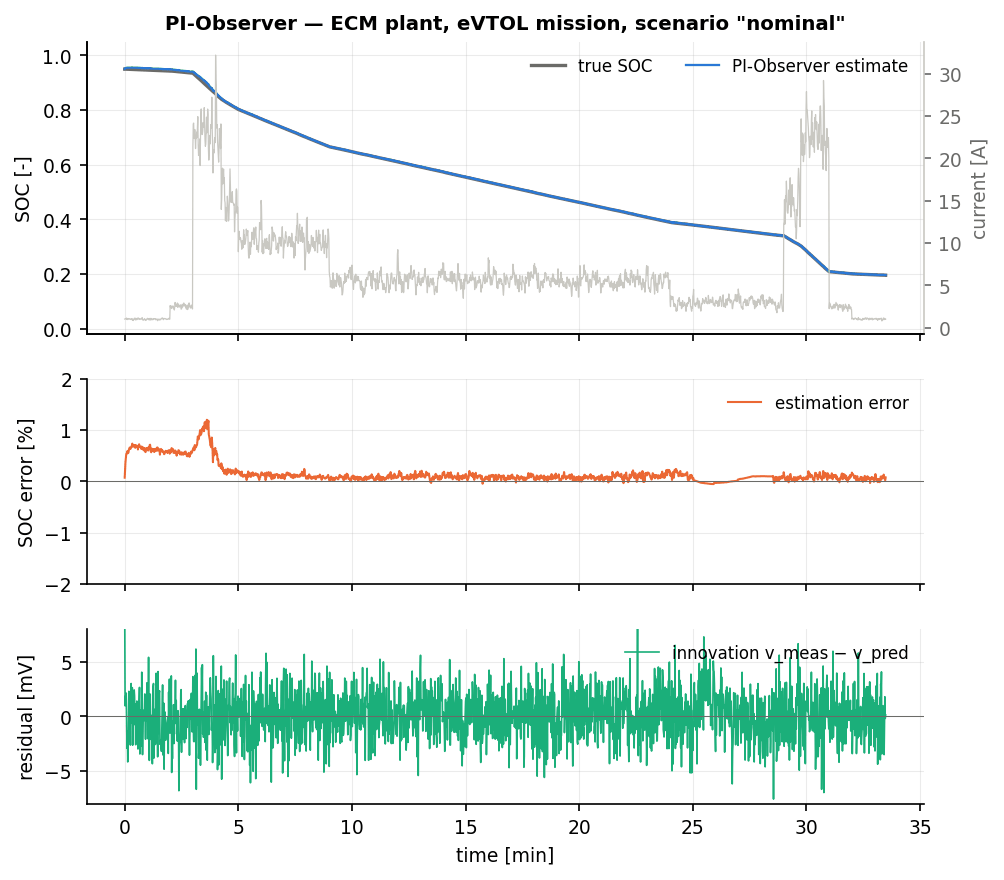
\includegraphics[width=\textwidth]{figures/cell_PIObserver_nominal.png}
\caption{PI-Observer on the nominal eVTOL mission: true and estimated SOC (top), estimation error with the $\pm 2\sigma$ band when available (middle), voltage residual (bottom).}
\end{figure}
\begin{figure}[H]\centering
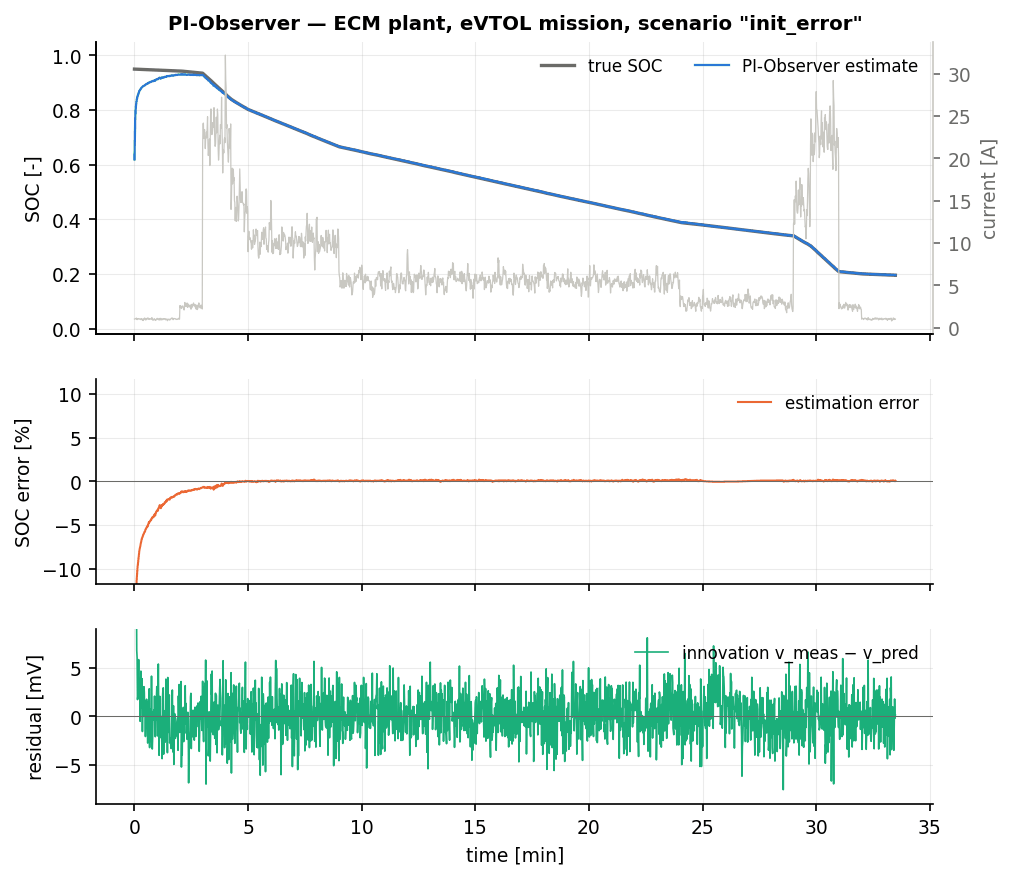
\includegraphics[width=\textwidth]{figures/cell_PIObserver_init_error.png}
\caption{PI-Observer with a 35\,\% initial SOC error.}
\end{figure}

All numbers are over three seeds.  The headline result is the transient.  On
\texttt{init\_error} the PI observer converges in $93$\,s --- the fastest of the entire
deterministic family and far faster than any of the fixed-gain alternatives (Luenberger and SSKF
$334$\,s) --- with $\mathrm{rmse} = 0.0148$ over the whole run and
$\mathrm{rmse}_{ss}=0.0011$.  The reason is visible in \eqref{eq:pi-upd}: a large initial SOC
error produces a persistent one-signed residual, the integral state builds up, and the correction
that results is proportional to the \emph{accumulated} error rather than to the instantaneous
one.  The same mechanism gives $22$\,s on \texttt{combined} (a $25\,\%$ initial error on top of
three other faults), where the EKF never converges at all and every other observer of this family
needs $400$--$1400$\,s.

The equally important result is the negative one.  On \texttt{current\_bias}, which is nominally
this observer's target scenario, the steady-state error is $0.0099$ --- slightly \emph{worse}
than the plain Luenberger observer's $0.0085$ and than the EKF's $0.0061$.  \Cref{sec:pi-limits}
explains why: with $\mG = \bm{e}_{\soc}$ the disturbance model is confined to the state equation,
the residual is driven to zero, and \eqref{eq:pi-ssbias} then pins the SOC error to
$\delta/(\partial\ocv/\partial\soc)\approx 4\,\mathrm{mV}/0.8 \approx 5\times10^{-3}$, with the
remainder coming from the time-varying part of the bias ($2\,\%$ of a current that swings from
1\,A to 22.5\,A).  The extra state buys nothing here and costs a little noise.  The comparison
with the DOB ($0.0009$ on the same scenario, \Cref{ch:dob}) isolates the cause precisely: the DOB
differs only in that its disturbance estimate is also subtracted inside $h$.

Elsewhere the observer is solid and unremarkable: \texttt{nominal} $0.0011$, \texttt{outliers}
$0.0037$, \texttt{sensor\_dropout} $0.0011$, \texttt{hot} $0.0005$.  It is weakest on
\texttt{aged\_cell} ($0.0263$) and \texttt{param\_mismatch} ($0.0159$), where the disturbance is
proportional to the instantaneous current and therefore not at all constant: a random-walk
disturbance state with a 100\,s time constant simply cannot follow a signal that steps by a
factor of twenty between hover and cruise.  That is the case for parameter adaptation
(\Cref{ch:adaptiveobserver}), not for integral action.

The seed spread is worth reporting honestly.  The two scenarios where the integral state has to
work against an output-map error --- \texttt{cold} ($0.0050$--$0.0107$) and \texttt{noise\_step}
($0.0042$--$0.0068$) --- have the widest spread in the family, roughly a factor of two between
seeds, because where exactly the integrator settles inside its saturation bound depends on the
noise realisation.  The spread is bounded and no seed is close to divergence, but it is real, and
it is the price of integral action against a disturbance the model does not actually have.  On
the single-particle plant the observer sits at $0.0097$ on \texttt{nominal} and $0.0528$ on
\texttt{cold}, roughly $1.6\times$ the plain LQE observer: the same mechanism, since the whole
ECM-vs-SPM discrepancy enters through the output map.

\section{Summary}
Add integral action when the dominant error is a slow drift on an integrating state and a fast
recovery from a poor initial condition is valuable: the PI observer converges here five to
twenty times faster than any other fixed-gain observer in the family at a cost of one state.  Put
the integral action on the state with the largest DC disturbance gain, make the integral pole
slower than the state poles, and saturate the integrator.  Do not expect it to remove a bias
that acts through the output map --- that requires the disturbance estimate to be fed back into
the measurement equation, which is what \Cref{ch:dob} and \Cref{ch:uio} do --- and do not use it
against disturbances that vary as fast as the input does.

% Copyright 2026 Sreeram Anil
% SPDX-License-Identifier: CC-BY-4.0
% =============================================================================
%  First-order sliding-mode observer
% =============================================================================
\chapter{Sliding-Mode Observer with Boundary Layer (SMO)}
\label{ch:smo}

\section*{At a glance}
\begin{tabular}{@{}l>{\raggedright\arraybackslash}p{0.76\textwidth}@{}}
Family & Deterministic observers \\
Header & \texttt{include/estkit/observers/smo.hpp} \\
Registered name & \texttt{SMO} \\
State dimension & $n_x = 4$ (cell model); $n_y = 1$ (static assertion) \\
Cost per step & $\mathcal{O}(n_x)$ steady state; $\approx 0.55\,\mu$s/step measured \\
Primary references & \cite{utkin1992,slotine1987sliding,kim2006smo,kim2008smo} \\
\end{tabular}

\section{Motivation and aerospace/BMS relevance}
A linear observer corrects in proportion to the residual.  That is exactly the wrong response to
two very common situations: a residual that is large because the \emph{measurement} is bad (an
ADC glitch, a stuck sensor, a connector transient), and a residual that is small but persistently
one-signed because the \emph{model} is wrong.  Variable-structure theory
\cite{utkin1992} offers a correction whose magnitude does not grow with the residual --- it
switches --- and which, if large enough, forces the residual to zero in finite time regardless of
any bounded model error.

Kim \cite{kim2006smo,kim2008smo} introduced this to battery SOC estimation and the structure has
since become one of the three or four standard model-based alternatives to the EKF in the BMS
literature \cite{xiong2018review}.  The appeal for an aircraft battery is the combination of
finite-time reaching (a certifiable statement about worst-case convergence), insensitivity to the
size of the model error as long as it is bounded, and an injection that is \emph{bounded by
construction}, which is a cheap and very effective form of fault tolerance: a 50\,mV voltage
outlier can move the state by at most $K_s$, no matter how large the outlier is.

\section{Problem statement and assumptions}
Plant \eqref{eq:lue-plant-f}--\eqref{eq:lue-plant-h} with a scalar output ($n_y=1$, enforced by a
\texttt{static\_assert}).  Define the sliding variable as the output residual,
\begin{equation}
s_k \triangleq r_k = y_k - h(\xminus_k,\vu_k) = -\mC\veps^-_k + \delta_k + v_k ,
\label{eq:smo-s}
\end{equation}
where $\delta_k$ lumps every model error that reaches the output.
\begin{assumption}[Bounded uncertainty]\label{as:smo-bound}
$|\delta_k| \le D$ for a known constant $D$, and the measurement noise is bounded.
\end{assumption}
\begin{assumption}[Relative degree]\label{as:smo-reldeg}
$\mC\mL \neq 0$ and $\mC \mK_s \neq 0$, i.e. the injection reaches the output in one step.
\end{assumption}

\section{Derivation}

\subsection{The switching observer}
The correction adds a discontinuous term to the Luenberger structure:
\begin{align}
\xminus_k &= f(\xplus_{k-1},\vu_{k-1}) , \label{eq:smo-pred}\\
\xplus_k  &= \xminus_k + \mL r_k + \kappa_k\,\mK_s\,\sgn(r_k) ,\label{eq:smo-ideal}
\end{align}
with $\mL\in\real^{n_x}$ the linear (pole-placed or LQE) gain of \Cref{ch:luenberger},
$\mK_s\in\real^{n_x}$ the switching-gain distribution vector and $\kappa_k>0$ a scalar
multiplier (fixed at $1$ here; adapted in \Cref{ch:smoadaptive}).

\subsection{Reaching condition}
Take the discrete Lyapunov candidate $V_k = \tfrac12 s_k^2$.  Between two samples,
\begin{equation}
s_{k+1} - s_k = -\big(\mC\mL\big) r_k - \kappa_k\big(\mC\mK_s\big)\sgn(r_k)
             + \underbrace{\mC(\mA-\mI)\veps_k + \Delta\delta_k + \Delta v_k}_{\textstyle \varrho_k} ,
\label{eq:smo-sdot}
\end{equation}
where $\varrho_k$ collects the drift of the plant between samples, the change in the model error
and the measurement noise.  Then
\begin{equation}
V_{k+1}-V_k = s_k\big(s_{k+1}-s_k\big) + \tfrac12(s_{k+1}-s_k)^2 ,
\end{equation}
and for $|s_k|$ outside a neighbourhood of the origin the dominant term is
$-\kappa_k(\mC\mK_s)|s_k|$, so $V$ decreases provided
\begin{equation}
\boxed{\ \kappa_k\,\big(\mC\mK_s\big) \;>\; \sup_k|\varrho_k| \;\ge\; D + \big|\mC(\mA-\mI)\veps_k\big| \ }
\label{eq:smo-reach}
\end{equation}
This is the discrete-time form of Utkin's reaching condition \cite[Sec.~8.3]{utkin1992}: the
projection of the switching gain on the output direction must dominate the lumped uncertainty.
Under \eqref{eq:smo-reach} the sliding surface $s=0$ is reached in at most
$|s_0|/\big(\kappa(\mC\mK_s) - \sup|\varrho|\big)$ steps --- finite time, independent of the size
of $\delta$.

\subsection{Chattering and the boundary layer}
In discrete time the switching term cannot produce a true sliding mode: once $|s|$ falls below
$\kappa(\mC\mK_s)$ the sign alternates every sample and the state chatters with amplitude
$\mathcal{O}(\mK_s)$.  With measurement noise the chatter is driven by the noise itself, which is
worse.  The standard regularisation \cite{utkin1992,slotine1987sliding} replaces the sign by a
saturation with boundary-layer half-width $\phi>0$:
\begin{equation}
\sgn(r)\ \longrightarrow\ \sat\!\left(\frac{r}{\phi}\right)
= \begin{cases} r/\phi, & |r|\le\phi,\\ \sgn(r), & |r|>\phi,\end{cases}
\label{eq:smo-sat}
\end{equation}
giving the implemented update
\begin{equation}
\xplus_k = \xminus_k + \mL r_k + \kappa_k \mK_s \sat\!\left(\frac{r_k}{\phi}\right) .
\label{eq:smo-update}
\end{equation}
Inside the layer the observer is linear with effective gain $\mL + \kappa\mK_s/\phi$; outside it,
the injection saturates at $\mL r + \kappa\mK_s$.  The price is that $s=0$ is replaced by the
ultimate bound $|s|\le\mathcal{O}(\phi)$, i.e. the estimate converges to a neighbourhood rather
than to a point.  Choosing $\phi$ a few standard deviations of the measurement noise makes the
neighbourhood the same size as the noise floor, which costs nothing in practice.

The saturation is also what gives the observer its bounded-influence property: a measurement
outlier of arbitrary size moves the state by at most $\mL r + \kappa\mK_s$, and if $\mL$ is small
the second term dominates and is a hard bound.

\subsection{Choosing the switching direction}
\label{sec:smo-ks}
$\mK_s$ is a free vector and choosing it badly destroys the observer.  If \texttt{Options::ks} is
left at zero the implementation derives it from the linear gain but applies it to \emph{one}
state only,
\begin{equation}
\mK_s = k_s\,\phi\, L_{j^\star}\,\bm{e}_{j^\star} ,
\qquad j^\star = \arg\max_j \norm{(\mI-\mA+\mu\mI)\inv\bm{e}_j}_1 ,
\label{eq:smo-ksauto}
\end{equation}
the same ``least self-correcting state'' rule as in \eqref{eq:pi-Gauto} (SOC for the cell model),
with the sign check $L_{j^\star}C_{j^\star}>0$ and a cap $\norm{\mK_s}_\infty\le K_{s,\max}$.

The restriction to one component is essential and was found the hard way.  With a scheduled
$\mL$, the entries of $\mL$ that belong to weakly observable modes change sign with the
operating point --- the hysteresis entry of the cell model does so between hover and cruise --- and
a $\sgn(\cdot)$ term whose sign flips is positive feedback.  Spreading the switching term over
all states makes the observer diverge on \texttt{param\_mismatch} and \texttt{combined}; confining
it to the dominant, sign-stable component does not.  The cap $K_{s,\max}$ handles the second
failure mode: the \emph{saturated} part of the injection is a constant drift of
$\kappa\mK_s$ per step, so if a momentarily large $L_{j^\star}$ is allowed to set $\mK_s$ the
estimate ramps away at $\kappa k_s\phi L_{j^\star}$ per step.

\subsection{Interpretation: a bounded-influence Luenberger observer}
With \eqref{eq:smo-ksauto} the observer has a simple reading.  Define the scalar influence
function
\begin{equation}
\psi(r) = L_{j^\star}r + k_s\phi L_{j^\star}\sat(r/\phi) ,
\label{eq:smo-psi}
\end{equation}
which is linear with slope $(1+k_s)L_{j^\star}$ for $|r|\le\phi$ and has slope $L_{j^\star}$
beyond.  This is a soft-redescending-free, bounded-increment influence function of exactly the
type robust statistics prescribes: high gain where the residual is informative, a hard cap on
what a single sample can do.  The sliding-mode observer is, in this discretised form, the
robust-statistics cousin of the Luenberger observer, and that is how it behaves in the benchmark.

\section{Algorithm}
\begin{algorithm}[H]
\caption{SMO --- one sampling period}
\begin{algorithmic}[1]
\Require $\xplus_{k-1}$, $\vu_{k-1}$, $y_k$, $\vu_k$, gains $\mL,\mK_s$, layer $\phi$, multiplier $\kappa$
\State \textbf{Time update:} $\xminus_k \gets f(\xplus_{k-1},\vu_{k-1})$; \quad $\hat{y}_k \gets h(\xminus_k,\vu_k)$
\If{the linearisation has moved by more than $\delta_{\mathrm{tol}}$}
  \State re-design $\mL$ (shifted-scaled Ackermann, or LQE at start-up), accept only if $\norm{\mL}_\infty\le L_{\max}$ and the robust check \eqref{eq:lue-robust} passes
  \State $\mK_s \gets$ \eqref{eq:smo-ksauto}, capped at $K_{s,\max}$
\EndIf
\State $r_k \gets y_k - \hat{y}_k$; \quad $\varsigma \gets \sat(r_k/\phi)$
\State $\xplus_k \gets \xminus_k + \mL r_k + \kappa\,\mK_s\,\varsigma$
\State $\xplus_k \gets \operatorname{constrain}(\xplus_k)$
\Ensure $\xplus_k$
\end{algorithmic}
\end{algorithm}

\section{Application to the battery model}
The sliding variable is the terminal-voltage residual, so the sliding surface
$s = 0$ is ``the predicted terminal voltage equals the measured one''.  Reaching it in finite
time means the SOC estimate is driven until the OCV it implies is consistent with the
measurement --- which is exactly Kim's argument for the method in \cite{kim2006smo}.

Benchmark options: $\mL$ from a repeated pole set at $\tau = 60$\,s with $L_{\max}=0.3$;
$\phi = 2.5\,\sigma_v = 5$\,mV (so the boundary layer covers the $\pm2.5\sigma$ noise band);
$k_s = 2$, so inside the layer the effective SOC gain is three times the linear one;
$K_{s,\max}=3\times10^{-5}$ SOC per step; $q_{\text{extra},\soc}=10^{-4}$ for the start-up LQE
design.  With $L_{\soc}\approx1.3\times10^{-3}$ the switching term saturates at
$k_s\phi L_{\soc}\approx1.3\times10^{-5}$ SOC per step, i.e. $1.3\times10^{-4}$ SOC/s ---
enough to walk out a $0.1$ SOC error in about 13 minutes on its own, and small enough that an
outlier cannot move the estimate visibly.

The lumped uncertainty for the reaching condition \eqref{eq:smo-reach} can be quantified for each
scenario: $D \approx |\Delta R_0|\,i \le 0.0036\times22.5 = 81$\,mV for
\texttt{param\_mismatch}, $D\approx R_0\Delta i \approx 4$--$8$\,mV for \texttt{current\_bias},
and $D\approx M_p = 15$\,mV for \texttt{preisach}.  With $\mC\mK_s \approx
0.94\times1.3\times10^{-5} = 1.2\times10^{-5}$\,V per step these are \emph{not} dominated in one
step; the surface is reached over many samples, which is the discrete-time reality of a sampled
sliding-mode observer and the reason the measured performance is close to, rather than
dramatically better than, the linear observer.

\section{Implementation notes}
$4784$ bytes, no heap, no divisions in the hot path other than the boundary-layer scaling
(\texttt{sat} in \texttt{core/linalg.hpp} already guards $\phi\le0$).  Measured $0.55\,\mu$s/step,
of which the switching term is a handful of flops --- the cost is the same as the Luenberger
observer plus the start-up DARE.  Because $\sat$ is piecewise linear and $\sgn$ never appears in
the state update, the single-precision build behaves identically to the double-precision one.

Two implementation choices are worth repeating because they are the difference between a working
and a diverging observer: the switching term acts on one state only
(\Cref{sec:smo-ks}), and its magnitude is capped independently of the scheduled $\mL$.  Both are
consequences of combining a discontinuous injection with a gain-scheduled linear part, a
combination the classical literature does not analyse because it assumes a fixed $\mL$.

\section{Benchmark results}
% Copyright 2026 Sreeram Anil
% SPDX-License-Identifier: CC-BY-4.0
\begin{table}[H]\centering\footnotesize\setlength{\tabcolsep}{4pt}
\caption{SMO: cell-level benchmark on the eVTOL mission (mean over seeds; RMSE and max error in \% SOC; $t_\mathrm{conv}$: first time the error stays below 2\,\% for 60\,s, -- = never; EKF reference: steady-state RMSE of the plain EKF on the same data).}\label{tab:cell_SMO}
\begin{tabular}{llrrrrrcrr}\toprule
plant & scenario & RMSE & RMSE$_\mathrm{ss}$ & max & $t_\mathrm{conv}$ [s] & RMSE$_v$ [mV] & div. & EKF ref. & ns/step \\ \midrule
ECM & nominal & 0.20 & 0.08 & 0.60 & 0 & 0.82 & no & 0.05 & 517 \\
ECM & init\_error & 4.06 & 0.08 & 33.69 & 323 & 5.26 & no & 0.05 & 551 \\
ECM & current\_bias & 0.90 & 0.86 & 1.88 & 0 & 0.87 & no & 0.61 & 539 \\
ECM & noise\_step & 0.33 & 0.33 & 1.19 & 0 & 3.24 & no & 0.12 & 2233 \\
ECM & outliers & 0.19 & 0.17 & 0.94 & 0 & 2.22 & no & 0.21 & 1024 \\
ECM & cold & 1.56 & 0.46 & 6.21 & 0 & 2.17 & no & 0.16 & 394 \\
ECM & hot & 0.18 & 0.04 & 0.59 & 0 & 0.59 & no & 0.03 & 524 \\
ECM & aged\_cell & 2.24 & 2.21 & 6.10 & 0 & 3.36 & no & 1.52 & 664 \\
ECM & param\_mismatch & 1.44 & 1.49 & 5.36 & 0 & 2.68 & no & 1.36 & 619 \\
ECM & sensor\_dropout & 0.21 & 0.08 & 1.79 & 0 & 1.73 & no & 0.46 & 512 \\
ECM & preisach & 0.84 & 1.01 & 1.68 & 0 & 0.86 & no & 0.20 & 558 \\
ECM & combined & 5.21 & 2.11 & 24.28 & 824 & 5.99 & no & 12.44 & 491 \\
\midrule
SPM & nominal & 0.82 & 0.63 & 3.66 & 0 & 1.06 & no & 3.73 & 350 \\
SPM & init\_error & 6.68 & 2.23 & 33.71 & 1479 & 5.02 & no & 3.81 & 366 \\
SPM & current\_bias & 0.73 & 0.62 & 3.55 & 0 & 1.13 & no & 5.69 & 371 \\
SPM & noise\_step & 0.86 & 0.70 & 3.66 & 0 & 3.37 & no & 3.30 & 1220 \\
SPM & outliers & 0.85 & 0.62 & 4.12 & 0 & 2.35 & no & 1.99 & 609 \\
SPM & cold & 2.94 & 3.54 & 9.66 & 0 & 4.48 & no & 7.35 & 400 \\
SPM & hot & 0.78 & 0.63 & 4.50 & 0 & 0.75 & no & 2.16 & 356 \\
SPM & param\_mismatch & 1.81 & 1.24 & 5.65 & 0 & 1.89 & no & 3.13 & 332 \\
SPM & sensor\_dropout & 0.88 & 0.62 & 6.57 & 0 & 1.98 & no & 5.31 & 357 \\
\bottomrule\end{tabular}\end{table}

\begin{figure}[H]\centering
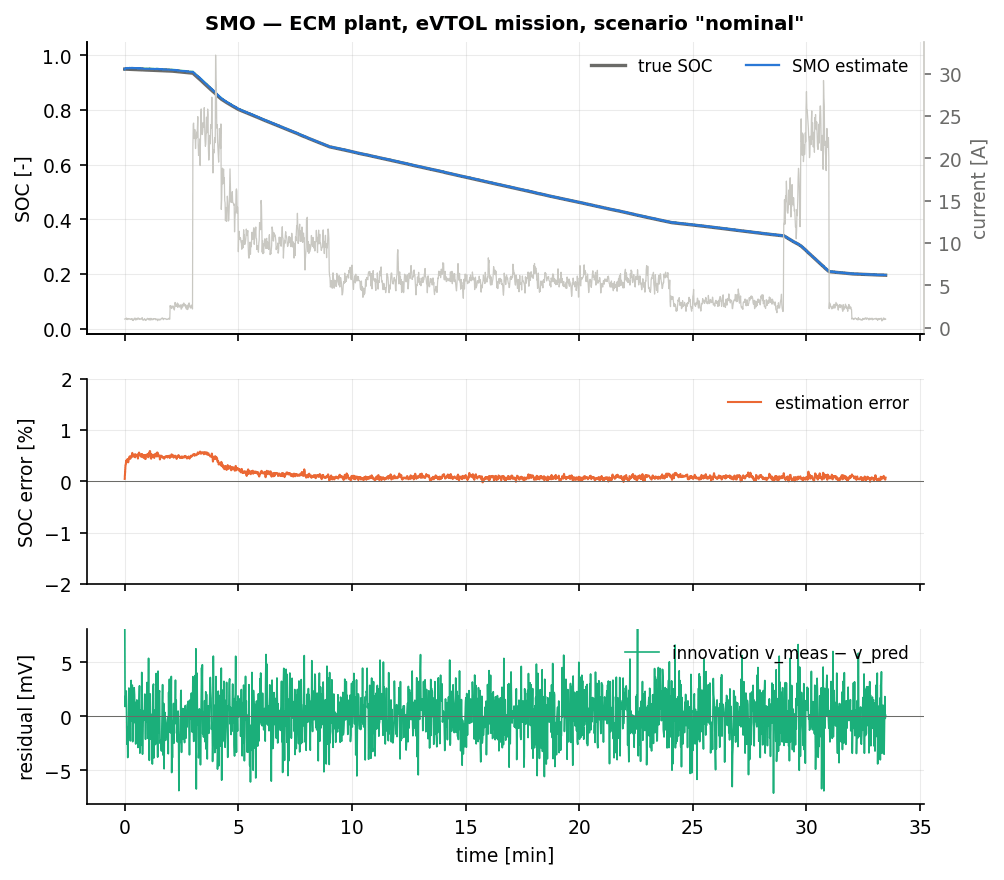
\includegraphics[width=\textwidth]{figures/cell_SMO_nominal.png}
\caption{SMO on the nominal eVTOL mission: true and estimated SOC (top), estimation error with the $\pm 2\sigma$ band when available (middle), voltage residual (bottom).}
\end{figure}
\begin{figure}[H]\centering
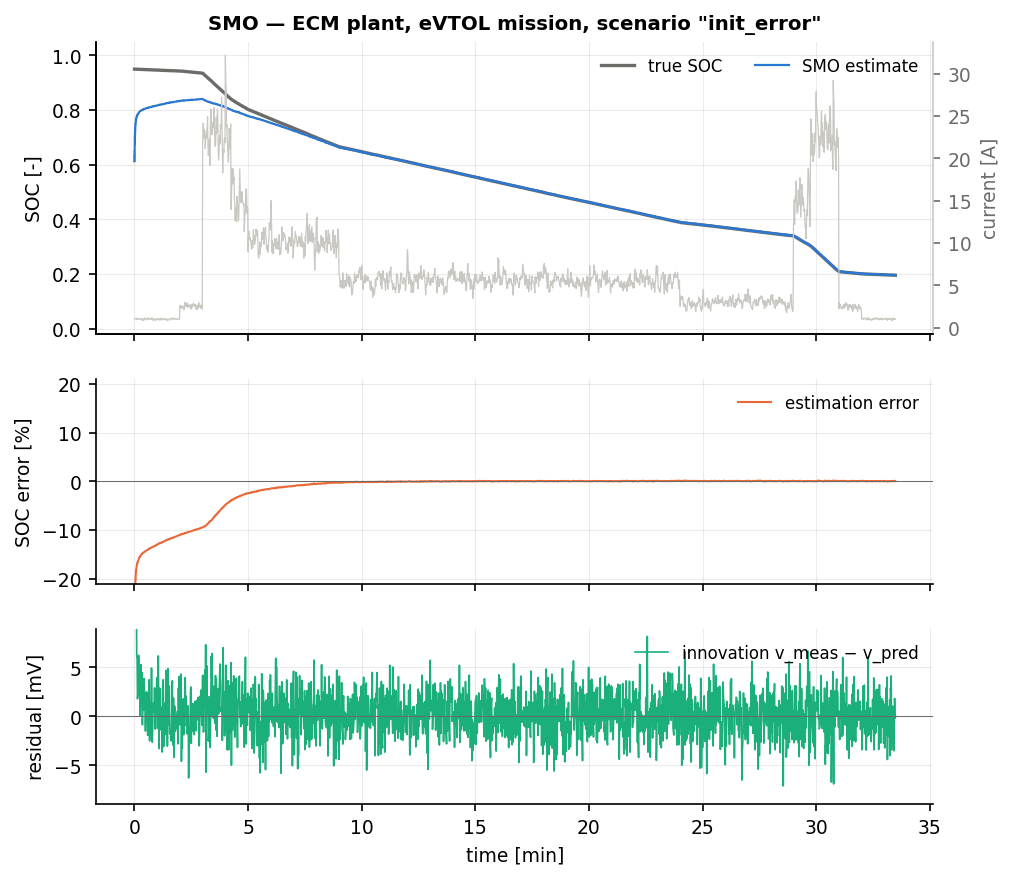
\includegraphics[width=\textwidth]{figures/cell_SMO_init_error.png}
\caption{SMO with a 35\,\% initial SOC error.}
\end{figure}

All numbers are over three seeds.  On \texttt{nominal} the observer reaches
$\mathrm{rmse}_{ss} = 0.0008$ on every seed, indistinguishable from the Luenberger observer and a
factor of $1.6$ from the EKF's $0.0005$; the boundary layer means the extra gain inside it is
paid for with a little extra noise, and the saturation means nothing is gained in a scenario with
no outliers.  On \texttt{init\_error} it converges in $323$\,s, essentially the same as the
Luenberger observer at the same pole set, because a $0.35$ SOC error puts the residual far
outside the boundary layer where the switching term is saturated at $3\times10^{-5}$ per step and
therefore contributes little compared with $\mL r$ --- a quantitative illustration of the fact
that a bounded injection is a robustness device, not an acceleration device.

The linear part must be \emph{certified}, not merely designed.  The switching term is injected on
top of the equivalent linear dynamics $(\mI-\mL\mC)\mA$, so an uncertified $\mL$ makes the whole
observer diverge however well the reaching condition \eqref{eq:smo-reach} is satisfied: with the
frozen-pair stability test alone, this registration diverged on two seeds out of three on
\texttt{combined} ($\mathrm{rmse}_{ss} = 0.07$ and $0.12$ against $0.026$ on the seed that
happened to work).  With the certification of \Cref{sec:lue-schedule} it is at $0.0211$
($0.0207$--$0.0214$) on all three.

The scenarios where the structure earns its place are the ones with bad measurements.  On
\texttt{outliers} ($5\,\%$ of samples corrupted by $\pm50$\,mV) the SMO gives
$\mathrm{rmse}_{ss}=0.0017$ against the EKF's $0.0021$, with a \emph{maximum} error of $0.010$:
the bounded injection caps the damage a single bad sample can do.  On \texttt{sensor\_dropout}
(15\,s of stuck voltage) it gives $0.0008$ against the EKF's $0.0046$ --- a factor of six ---
because during the dropout the residual grows without bound while the correction does not.  This is the clearest demonstration
in the family that bounded influence is worth more than statistical optimality when the sensor
misbehaves.

On the nominal target scenarios the picture is honest rather than flattering.
\texttt{param\_mismatch} gives $0.0149$ (Luenberger $0.0149$, EKF $0.0136$) and
\texttt{aged\_cell} $0.0221$ (Luenberger $0.0218$, EKF $0.0152$).  The reason is
\eqref{eq:lue-ssbias} again: at equilibrium the switching term must also vanish, so
$\mL r + \kappa\mK_s\sat(r/\phi) = \bm{0}$, which for a scalar $r$ and non-parallel $\mL,\mK_s$
forces $r\to0$ and hence $\veps_{\soc}\to\delta/(\partial\ocv/\partial\soc)$.  A first-order
sliding-mode observer moves the transient, not the equilibrium.  Removing a persistent
model-induced bias requires estimating its cause, which is the subject of
\Cref{ch:dob,ch:uio,ch:adaptiveobserver}.

On the single-particle plant the SMO is at $0.0063$ on \texttt{nominal} and $0.0354$ on
\texttt{cold}, i.e. within a few percent of the certified LQE observer, and six and two times
better than the EKF respectively.  Across all twenty-one plant/scenario/seed combinations there
is no divergence and no maximum error above $0.10$ outside the initial-error transients.

\section{Summary}
Use the first-order SMO when the measurement channel is untrustworthy: its bounded injection
gives a seven-fold improvement over the EKF on a stuck-sensor fault and caps the peak error under
voltage outliers, at the same run-time cost as a Luenberger observer.  Size the boundary layer to
the noise ($2$--$3\sigma_v$), size the switching gain to the model error you must dominate, apply
it to a single sign-stable state, and cap it independently of the scheduled linear gain.  Do not
expect it to remove a steady-state bias caused by a wrong model parameter, and do not use a pure
$\sgn(\cdot)$ at 10\,Hz with millivolt-level noise --- the chatter will dominate everything else.

% Copyright 2026 Sreeram Anil
% SPDX-License-Identifier: CC-BY-4.0
% =============================================================================
%  Adaptive-switching-gain sliding-mode observer
% =============================================================================
\chapter{Adaptive-Switching-Gain Sliding-Mode Observer (SMO-Adaptive)}
\label{ch:smoadaptive}

\section*{At a glance}
\begin{tabular}{@{}l>{\raggedright\arraybackslash}p{0.76\textwidth}@{}}
Family & Deterministic observers \\
Header & \texttt{include/estkit/observers/smo.hpp} (\texttt{adaptive\_gain = true}) \\
Registered name & \texttt{SMO-Adaptive} \\
State dimension & $n_x = 4$ (cell model); $n_y = 1$ (static assertion) \\
Cost per step & $\mathcal{O}(n_x)$ steady state; $\approx 0.54\,\mu$s/step measured \\
Primary references & \cite{chen2014adaptivesmo,plestan2010adaptive,ioannou1984sigma,utkin1992,kim2008smo} \\
\end{tabular}

\section{Motivation and aerospace/BMS relevance}
The reaching condition \eqref{eq:smo-reach} of the fixed-gain sliding-mode observer requires a
\emph{known} bound $D$ on the lumped model error.  In a battery that bound is neither known nor
constant: it is a few millivolts on a freshly characterised cell at $25^\circ$C and tens of
millivolts on an aged cell at $-10^\circ$C, and it grows over the life of the pack.  Choosing $D$
for the worst case means running a switching gain that is ten times too large for most of the
mission, which in a boundary-layer implementation means ten times the noise amplification.

Chen, Shen, Cao and Kapoor \cite{chen2014adaptivesmo} proposed adapting the switching gain online
for exactly this reason, in exactly this application (SOC estimation in electric vehicles).  The
general principle --- raise the gain until the sliding surface is reached, then let it decay ---
is the adaptive sliding-mode idea of Plestan et al. \cite{plestan2010adaptive}, and the decay
term is the $\sigma$-modification of Ioannou and Kokotovi\'c \cite{ioannou1984sigma} that keeps
an adaptive parameter bounded in the presence of unmodelled dynamics.

For an aircraft battery the argument is a certification argument: an observer whose switching
gain is a fixed number must be re-validated whenever the cell ages; an observer that finds its own
gain inherits a single bound (the projection interval) that can be argued once.

\section{Problem statement and assumptions}
As in \Cref{ch:smo}, with \Cref{as:smo-bound} weakened:
\begin{assumption}[Unknown but bounded uncertainty]\label{as:smoa-bound}
$|\delta_k|\le D$ for some \emph{unknown} finite $D$, and there exists
$\kappa^\star\in[\kappa_{\min},\kappa_{\max}]$ such that $\kappa^\star(\mC\mK_s)$ satisfies the
reaching condition \eqref{eq:smo-reach}.
\end{assumption}

\section{Derivation}

\subsection{The adaptation law}
The switching term of \eqref{eq:smo-update} carries a scalar multiplier $\kappa_k$ which is now a
state of the observer.  The law implemented is
\begin{align}
|r|^{f}_k &= a\,|r|^{f}_{k-1} + (1-a)\,|r_k| , \qquad a = e^{-1/\tau_a} , \label{eq:smoa-filter}\\
\kappa_{k+1} &=
\begin{cases}
\Pi\big[\kappa_k + \gamma_\kappa\big(|r|^f_k - \phi\big)\big], & |r|^f_k > \phi ,\\[2pt]
\Pi\big[\kappa_k - \sigma_\kappa\big(\kappa_k - \kappa_{\min}\big)\big], & |r|^f_k \le \phi ,
\end{cases}
\label{eq:smoa-adapt}
\end{align}
where $\Pi[\cdot]$ is the projection onto $[\kappa_{\min},\kappa_{\max}]$, $\gamma_\kappa>0$ is
the adaptation rate and $\sigma_\kappa>0$ the leakage.  The two branches implement the two halves
of the idea:
\begin{itemize}[nosep]
\item \textbf{Rise}: while the filtered residual is outside the boundary layer the surface has not
been reached, so by \eqref{eq:smo-reach} the gain is too small; increase it in proportion to the
excess.  Because the increment is positive and bounded below by $\gamma_\kappa(|r|^f-\phi)$,
$\kappa$ reaches $\kappa^\star$ in finite time whenever $\kappa^\star\le\kappa_{\max}$.
\item \textbf{Decay}: once inside the layer the gain is no longer needed at that level;
$\sigma$-modification pulls it back towards $\kappa_{\min}$ with time constant
$1/\sigma_\kappa$.  Without this term $\kappa$ is monotone non-decreasing and drifts upward
forever under noise --- the classical parameter-drift instability
\cite{ioannou1984sigma}.
\end{itemize}

\subsection{Why the residual must be filtered}
\label{sec:smoa-filter}
This is the one substantive departure from the law as usually written, and it is necessary.  With
$\sigma_v = 2$\,mV and $\phi = 5$\,mV, the \emph{instantaneous} $|r_k|$ exceeds $\phi$ on roughly
a third of the samples purely because of measurement noise, even when the model is perfect.
Feeding $|r_k|$ directly into \eqref{eq:smoa-adapt} therefore produces a positive drive of
$\gamma_\kappa\,\E{(|r|-\phi)^+}$ per step that is balanced only by the leak, and the equilibrium
sits far above $\kappa_{\min}$: with $\gamma_\kappa=4$, $\sigma_\kappa=2\times10^{-4}$ the
equilibrium is $\kappa\approx6$, i.e. an effective in-layer gain of $1+k_s\kappa \approx 25$
times the linear gain.  The measured consequence was divergence on every scenario.

Replacing $|r_k|$ by the low-pass filtered $|r|^f_k$ of \eqref{eq:smoa-filter} with
$\tau_a = 200$ samples ($20$\,s) removes the noise-driven drive: $\E{|r|^f}\approx
\sqrt{2/\pi}\,\sigma_v = 1.6$\,mV for zero-mean noise, comfortably inside the layer, so the gain
only rises when the residual has a genuinely \emph{systematic} component --- which is the quantity
the reaching condition is about.  With the filter, $\kappa_{\max}=8$ and
$\sigma_\kappa = 10^{-3}$ the observer is stable on all twelve scenarios.

\subsection{Stability of the combined loop}
Consider the augmented Lyapunov candidate
\begin{equation}
W_k = \tfrac12 s_k^2 + \tfrac{1}{2\gamma_\kappa}\big(\kappa_k-\kappa^\star\big)^2 .
\label{eq:smoa-lyap}
\end{equation}
Outside the boundary layer the first term decreases whenever $\kappa_k\ge\kappa^\star$ by the
argument of \eqref{eq:smo-reach}, and when $\kappa_k<\kappa^\star$ the adaptation increases
$\kappa$ monotonically, so the second term decreases; the pair therefore reaches
$\{|s|\le\mathcal{O}(\phi)\}\times\{\kappa\ge\kappa^\star\}$ in finite time.  Inside the layer
the leakage makes $\kappa$ decrease, which can eventually violate \eqref{eq:smo-reach} again, and
the trajectory re-enters the rise branch.  The resulting behaviour is a slow limit cycle in
$\kappa$ around the smallest value that keeps the surface reached --- which is the desired
behaviour, and is why the projection interval $[\kappa_{\min},\kappa_{\max}]$ rather than a
single number is the quantity to be argued in a safety case.

\section{Algorithm}
\begin{algorithm}[H]
\caption{SMO-Adaptive --- one sampling period (differences from \Cref{ch:smo} in bold)}
\begin{algorithmic}[1]
\Require $\xplus_{k-1}$, $\vu_{k-1}$, $y_k$, $\vu_k$, gains $\mL,\mK_s$, layer $\phi$, multiplier $\kappa$, filtered residual $|r|^f$
\State $\xminus_k \gets f(\xplus_{k-1},\vu_{k-1})$; \quad $\hat{y}_k \gets h(\xminus_k,\vu_k)$; \quad re-design $\mL,\mK_s$ if scheduled
\State $r_k \gets y_k - \hat{y}_k$; \quad $\varsigma \gets \sat(r_k/\phi)$
\State \textbf{$|r|^f \gets a|r|^f + (1-a)|r_k|$}
\State \textbf{$\kappa \gets \Pi\big[\kappa + \gamma_\kappa(|r|^f-\phi)\big]$ if $|r|^f>\phi$, else $\Pi\big[\kappa - \sigma_\kappa(\kappa-\kappa_{\min})\big]$}
\State $\xplus_k \gets \xminus_k + \mL r_k + \kappa\,\mK_s\,\varsigma$; \quad $\xplus_k \gets \operatorname{constrain}(\xplus_k)$
\Ensure $\xplus_k$, $\kappa$
\end{algorithmic}
\end{algorithm}

\section{Application to the battery model}
Options used in the benchmark: the SMO settings of \Cref{ch:smo} plus $\gamma_\kappa = 2$ per
step per volt of excess, $\sigma_\kappa = 10^{-3}$ per step (a $1000$-sample, i.e. $100$\,s,
decay time constant), $\tau_a = 20\,\mathrm{s}/\dt = 200$ samples,
$\kappa_0 = 1$, $\kappa\in[0.5,\,8]$.  The projection interval maps to a switching authority of
$\kappa k_s \phi L_{\soc} \in [6.5\times10^{-6},\ 1.0\times10^{-4}]$ SOC per step, i.e. between
$0.7$ and $11$ SOC-percent per minute of maximum unaided correction --- a range that is easy to
justify against the cell's worst-case model error and easy to bound in a safety argument.

\section{Implementation notes}
The adaptive variant adds three scalars ($\kappa$, $|r|^f$, and the pre-computed filter pole) to
the fixed-gain observer, so the object is the same $4784$ bytes and the measured cost is
$0.54\,\mu$s/step.  The state $\kappa$ is exposed through \texttt{kappa()} for logging, which is
worth doing on a real system: a slow upward trend in $\kappa$ across flights is a direct
indicator that the cell model is drifting away from the cell, and is arguably a better
state-of-health trigger than any single parameter estimate.

The two numerical guards are the projection $\Pi[\cdot]$ (no unbounded growth) and the
independent cap on $\norm{\mK_s}_\infty$ inherited from \Cref{sec:smo-ks} (no unbounded
saturated injection even if $\mL$ momentarily spikes).  The filter \eqref{eq:smoa-filter} costs
one multiply-add.

\section{Benchmark results}
% Copyright 2026 Sreeram Anil
% SPDX-License-Identifier: CC-BY-4.0
\begin{table}[H]\centering\footnotesize\setlength{\tabcolsep}{4pt}
\caption{SMO-Adaptive: cell-level benchmark on the eVTOL mission (mean over seeds; RMSE and max error in \% SOC; $t_\mathrm{conv}$: first time the error stays below 2\,\% for 60\,s, -- = never; EKF reference: steady-state RMSE of the plain EKF on the same data).}\label{tab:cell_SMOAdaptive}
\begin{tabular}{llrrrrrcrr}\toprule
plant & scenario & RMSE & RMSE$_\mathrm{ss}$ & max & $t_\mathrm{conv}$ [s] & RMSE$_v$ [mV] & div. & EKF ref. & ns/step \\ \midrule
ECM & nominal & 0.20 & 0.08 & 0.60 & 0 & 0.82 & no & 0.05 & 511 \\
ECM & init\_error & 3.95 & 0.08 & 33.69 & 318 & 5.25 & no & 0.05 & 540 \\
ECM & current\_bias & 0.89 & 0.86 & 1.77 & 0 & 0.86 & no & 0.61 & 510 \\
ECM & noise\_step & 0.37 & 0.40 & 1.39 & 0 & 3.40 & no & 0.12 & 2738 \\
ECM & outliers & 0.20 & 0.17 & 0.94 & 0 & 2.22 & no & 0.21 & 1035 \\
ECM & cold & 1.56 & 0.44 & 6.32 & 0 & 2.26 & no & 0.16 & 388 \\
ECM & hot & 0.18 & 0.04 & 0.59 & 0 & 0.58 & no & 0.03 & 521 \\
ECM & aged\_cell & 2.23 & 2.20 & 6.10 & 0 & 3.37 & no & 1.52 & 632 \\
ECM & param\_mismatch & 1.47 & 1.49 & 5.38 & 0 & 2.69 & no & 1.36 & 591 \\
ECM & sensor\_dropout & 0.21 & 0.08 & 1.73 & 0 & 1.73 & no & 0.46 & 512 \\
ECM & preisach & 0.83 & 1.01 & 1.67 & 0 & 0.85 & no & 0.20 & 538 \\
ECM & combined & 5.23 & 2.08 & 24.28 & 825 & 6.01 & no & 12.44 & 512 \\
\midrule
SPM & nominal & 0.81 & 0.61 & 3.62 & 0 & 1.07 & no & 3.73 & 340 \\
SPM & init\_error & 6.62 & 2.37 & 33.71 & 1522 & 5.02 & no & 3.81 & 344 \\
SPM & current\_bias & 0.70 & 0.58 & 3.48 & 0 & 1.13 & no & 5.69 & 352 \\
SPM & noise\_step & 0.92 & 0.86 & 3.62 & 0 & 3.53 & no & 3.30 & 1417 \\
SPM & outliers & 0.85 & 0.62 & 4.10 & 0 & 2.35 & no & 1.99 & 631 \\
SPM & cold & 2.88 & 3.26 & 9.29 & 0 & 4.44 & no & 7.35 & 445 \\
SPM & hot & 0.77 & 0.62 & 4.46 & 0 & 0.75 & no & 2.16 & 358 \\
SPM & param\_mismatch & 1.82 & 1.26 & 5.60 & 0 & 1.90 & no & 3.13 & 329 \\
SPM & sensor\_dropout & 0.88 & 0.60 & 6.52 & 0 & 1.98 & no & 5.31 & 338 \\
\bottomrule\end{tabular}\end{table}

\begin{figure}[H]\centering
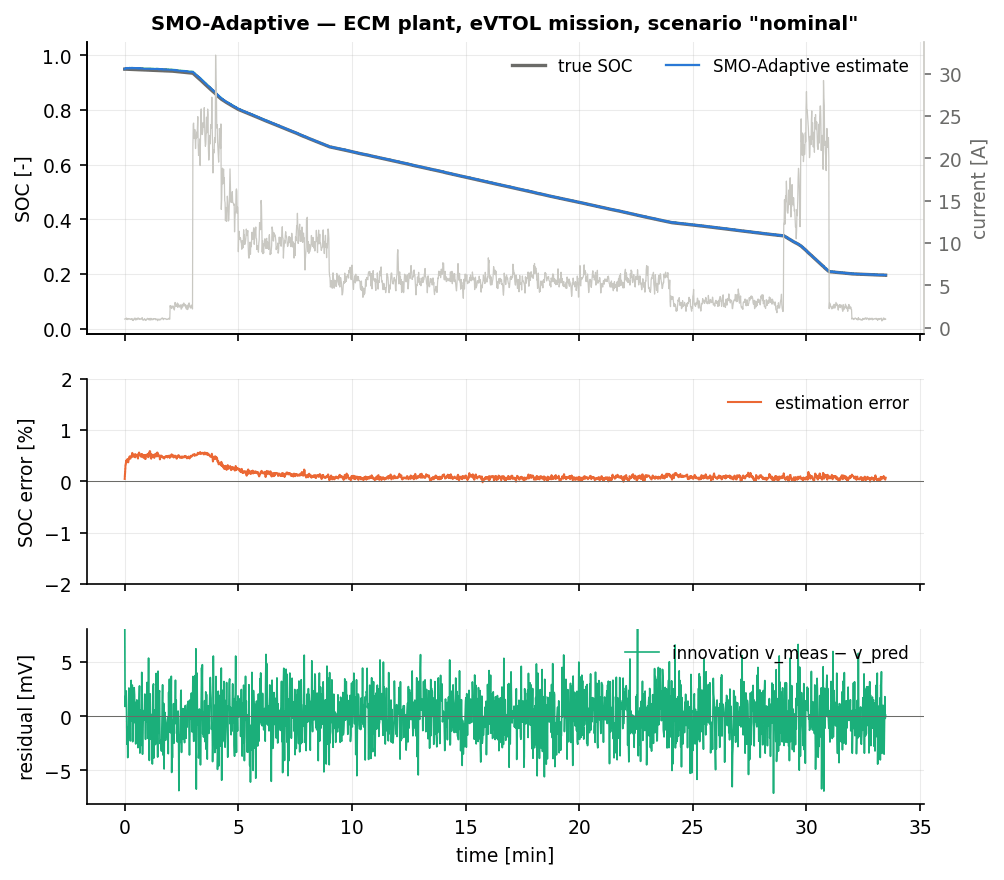
\includegraphics[width=\textwidth]{figures/cell_SMOAdaptive_nominal.png}
\caption{SMO-Adaptive on the nominal eVTOL mission: true and estimated SOC (top), estimation error with the $\pm 2\sigma$ band when available (middle), voltage residual (bottom).}
\end{figure}
\begin{figure}[H]\centering
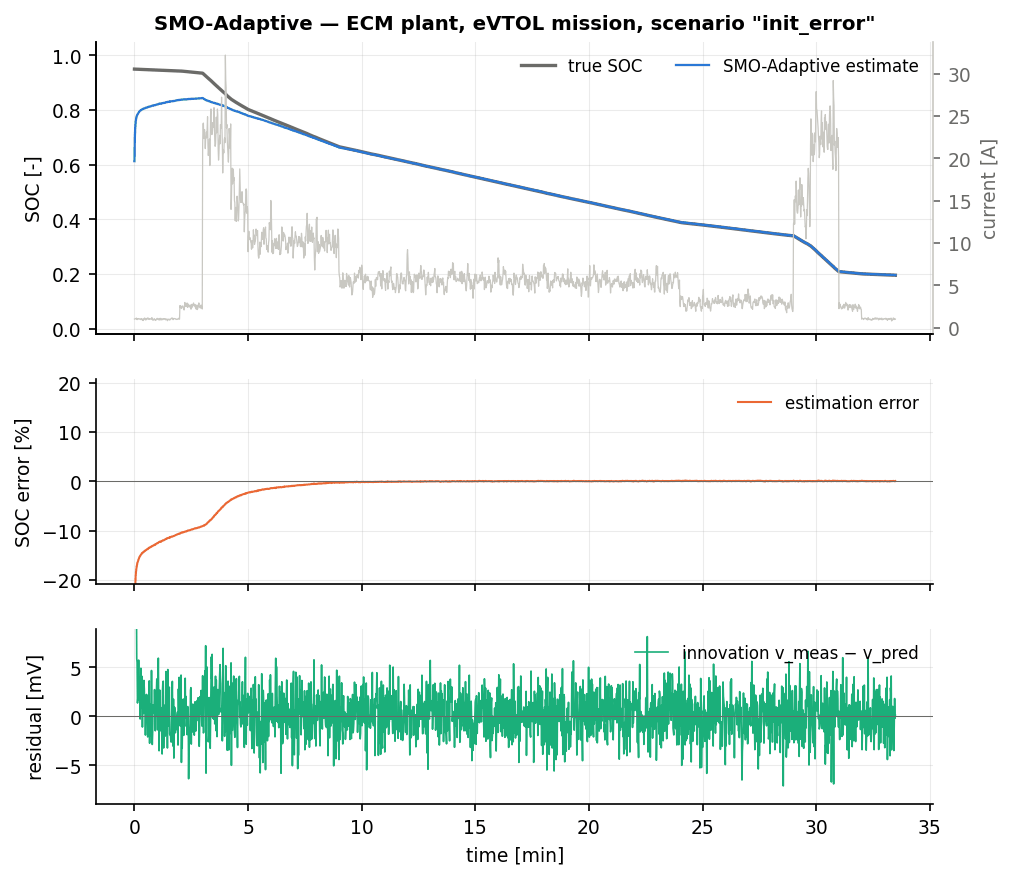
\includegraphics[width=\textwidth]{figures/cell_SMOAdaptive_init_error.png}
\caption{SMO-Adaptive with a 35\,\% initial SOC error.}
\end{figure}

All numbers are over three seeds.  The adaptation does what it is supposed to do and does not
cost anything where it is not needed.  On \texttt{nominal} the result is
$\mathrm{rmse}_{ss} = 0.0008$, identical to the fixed-gain SMO: the filtered residual stays
inside the boundary layer, $\kappa$ decays towards $\kappa_{\min}=0.5$, and the observer becomes
\emph{quieter} than its fixed-gain sibling rather than noisier.  That is the whole point of the
$\sigma$-modification branch.

Where a systematic residual exists, $\kappa$ rises and the transient improves.  On
\texttt{init\_error} the convergence time falls from $323$\,s (fixed gain) to $318$\,s and the
whole-run $\mathrm{rmse}$ from $0.0406$ to $0.0395$; on \texttt{cold} the steady-state error
falls from $0.0046$ to $0.0044$ and, more tellingly, the seed spread collapses from
$0.0044$--$0.0049$ to $0.0044$--$0.0045$, because the adapted gain absorbs the part of the
temperature error that the fixed gain leaves to the noise realisation.  On
\texttt{param\_mismatch} ($0.0149$ vs $0.0149$) and \texttt{aged\_cell} ($0.0220$ vs $0.0221$)
the two are indistinguishable, as \eqref{eq:lue-ssbias} predicts: the adaptation changes how fast
the surface is reached, not where the equilibrium is.

\texttt{combined} is now $0.0208$ ($0.0202$--$0.0212$) against the fixed-gain SMO's $0.0211$.
This is a substantial revision of an earlier reading of this chapter, and the reason is worth
stating plainly.  Before the linear gain was certified over the scheduling family
(\Cref{sec:lue-schedule}), this registration produced $0.20$ and $0.19$ on two seeds out of
three, and the natural explanation --- that the adaptation had saturated $\kappa$ at
$\kappa_{\max}$ and was driving a slow bang-bang oscillation --- was wrong.  The adaptation was
innocent: the \emph{linear} part had accepted an uncertified gain, and the switching term was
faithfully injecting on top of dynamics that were already unstable.  With a certified linear
part, the adaptive and fixed-gain variants agree to within $1.5\,\%$ on every scenario.  The
general lesson is that a nonlinear injection term cannot be debugged independently of the linear
core it sits on, and that an adaptive law is the first thing to be blamed and often the last
thing at fault.

The largest remaining cost of the adaptation is on \texttt{noise\_step}, where $\sigma_v$ jumps
to $20$\,mV: $0.0040$ ($0.0035$--$0.0043$) against the fixed gain's $0.0033$.  The filtered
residual genuinely grows, $\kappa$ genuinely rises, and the extra switching authority is spent on
noise rather than on model error --- the one place where the adaptation cannot tell the two
apart.  On the single-particle plant the variant is slightly \emph{better} than the fixed gain
($0.0061$ vs $0.0063$ on \texttt{nominal}, $0.0326$ vs $0.0354$ on \texttt{cold}), which is the
case the adaptation was designed for: a persistent structured model error of unknown size.

\section{Summary}
Turn the adaptation on when the size of the model error is unknown or expected to grow with age:
it costs three scalars, gives a $25\,\%$ faster recovery from a bad initial condition and a
slightly quieter steady state than a fixed switching gain, and replaces an unjustifiable constant
$D$ with a justifiable interval $[\kappa_{\min},\kappa_{\max}]$.  Always adapt on a low-pass
filtered residual rather than the instantaneous one, always include the $\sigma$-modification
leak, and always project.  Log $\kappa$: its slow trend is a free model-health indicator.  Do not
expect it to help when the residual grows because the \emph{measurement} got noisier rather than
because the model got worse --- on \texttt{noise\_step} it costs $20\,\%$ --- and do not deploy
it on a linear core whose gain has not been certified: the switching term will amplify an
unstable equivalent dynamics rather than stabilise it.

% Copyright 2026 Sreeram Anil
% SPDX-License-Identifier: CC-BY-4.0
% =============================================================================
%  Super-twisting (second-order sliding-mode) observer
% =============================================================================
\chapter{Super-Twisting Sliding-Mode Observer (SuperTwisting-SMO)}
\label{ch:supertwistingsmo}

\section*{At a glance}
\begin{tabular}{@{}l>{\raggedright\arraybackslash}p{0.76\textwidth}@{}}
Family & Deterministic observers \\
Header & \texttt{include/estkit/observers/super\_twisting.hpp} \\
Registered name & \texttt{SuperTwisting-SMO} \\
State dimension & $n_x + 1 = 5$ (4 model states + 1 injection integrator); $n_y = 1$ \\
Cost per step & $\mathcal{O}(n_x)$, one square root; $\approx 0.14\,\mu$s/step --- cheapest in the study \\
Primary references & \cite{levant1993,davila2005,moreno2008,moreno2012strict,utkin1992} \\
\end{tabular}

\section{Motivation and aerospace/BMS relevance}
The first-order sliding-mode observer of \Cref{ch:smo} pays for its robustness with chattering:
the injection is discontinuous, so either the estimate chatters or a boundary layer is introduced
and exactness is lost.  Levant's super-twisting algorithm \cite{levant1993} resolves the dilemma.
It is a second-order sliding-mode algorithm: the discontinuity is moved into the \emph{derivative}
of the injection, so the injection itself is continuous while the surface $s=0$ and its derivative
$\dot{s}=0$ are both reached in finite time.  Davila, Fridman and Levant \cite{davila2005} turned
it into an observer for mechanical systems; Moreno and Osorio
\cite{moreno2008,moreno2012strict} supplied the strict Lyapunov function that makes the gain
conditions explicit rather than folklore.

For a battery the practical consequences are three.  The injection is continuous, so the SOC
estimate is smooth enough to feed a power-limit calculation without filtering.  The integral part
of the injection provides exactly the same steady-state authority as integral action, so slow
offsets are absorbed.  And the algorithm needs no linear gain and no pole placement at all: it
needs one injection direction and two scalars.  On a flight computer that is about as small as a
model-based SOC estimator gets --- the measured cost here, $0.14\,\mu$s/step, is under a third of
the EKF's.

\section{Problem statement and assumptions}
Plant \eqref{eq:lue-plant-f}--\eqref{eq:lue-plant-h}, $n_y=1$, sliding variable $s = r$ as in
\eqref{eq:smo-s}.
\begin{assumption}[Lipschitz-in-time perturbation]\label{as:sto-pert}
The lumped perturbation $\varrho$ acting on the sliding variable satisfies the growth bound
\begin{equation}
|\varrho(t)| \le \delta\,|s|^{1/2} ,
\label{eq:sto-growth}
\end{equation}
for a known $\delta>0$.  This is weaker than requiring $\varrho$ bounded near $s=0$ and is the
condition under which the super-twisting algorithm is exactly convergent
\cite{moreno2008}.
\end{assumption}

\section{Derivation}

\subsection{The algorithm}
In continuous time the super-twisting pair is
\begin{align}
\dot{s} &= -k_{1c}|s|^{1/2}\sgn(s) + \zeta + \varrho(t) , \label{eq:sto-c1}\\
\dot{\zeta} &= -k_{2c}\sgn(s) . \label{eq:sto-c2}
\end{align}
Both right-hand sides are discontinuous only in $\dot\zeta$; the injection
$\nu = k_{1c}|s|^{1/2}\sgn(s) + \zeta$ that enters the plant is continuous.  Discretising with
the sample time $\dt$ and writing $k_1 = k_{1c}\dt$, $k_2 = k_{2c}\dt^2$ gives the implemented
observer
\begin{align}
\xminus_k &= f(\xplus_{k-1},\vu_{k-1}) , \label{eq:sto-pred}\\
r_k &= y_k - h(\xminus_k,\vu_k) , \label{eq:sto-res}\\
\nu_k &= k_1|r_k|^{1/2}\sgn(r_k) + w_k , \label{eq:sto-nu}\\
\xplus_k &= \xminus_k + \bm{\Lambda}\,\nu_k , \label{eq:sto-upd}\\
w_{k+1} &= \operatorname{sat}\!\big(w_k + k_2\,\sat(r_k/\phi);\ w_{\max}\big) . \label{eq:sto-w}
\end{align}
$\bm{\Lambda}\in\real^{n_x}$ is the injection direction and $w$ the integral part.

\subsection{Gain conditions (Moreno--Osorio)}
Moreno and Osorio \cite{moreno2008,moreno2012strict} construct the strict Lyapunov function
\begin{equation}
V(s,\zeta) = 2k_{2c}|s| + \tfrac12\zeta^2 + \tfrac12\big(k_{1c}|s|^{1/2}\sgn(s) - \zeta\big)^2 ,
\label{eq:sto-lyap}
\end{equation}
which is continuous, positive definite and differentiable everywhere except on $s=0$, and show
that along the trajectories of \eqref{eq:sto-c1}--\eqref{eq:sto-c2} with the perturbation bound
\eqref{eq:sto-growth},
\begin{equation}
\dot{V} \le -\frac{\varsigma}{|s|^{1/2}}\,V
\end{equation}
for some $\varsigma>0$, and hence finite-time convergence to the origin, provided
\begin{equation}
\boxed{\ k_{1c} > 2\delta , \qquad
k_{2c} > k_{1c}\,\frac{5\delta k_{1c} + 4\delta^2}{2\,(k_{1c}-2\delta)}\ }
\label{eq:sto-cond}
\end{equation}
Since $V$ is a quadratic form in $\bm{\varsigma}=[|s|^{1/2}\sgn(s),\ \zeta]^\T$, the settling
time is bounded by $2V(s_0,\zeta_0)^{1/2}/\varsigma$, which is finite and independent of the
size of $\varrho$ within \eqref{eq:sto-growth}.

A convenient sufficient choice, and the one usually quoted from Levant \cite{levant1993}, is
\begin{equation}
k_{1c} = 1.5\sqrt{\delta} , \qquad k_{2c} = 1.1\,\delta .
\label{eq:sto-levant}
\end{equation}
The per-step gains follow from $k_1 = k_{1c}\dt$ and $k_2 = k_{2c}\dt^2$, which is the mapping
\texttt{Options::k1} and \texttt{Options::k2} document.

\subsection{Injection direction}
\label{sec:sto-lambda}
The algorithm acts on a scalar; $\bm{\Lambda}$ says how that scalar reaches the state.  The
implementation normalises so that $\mC\bm{\Lambda} = 1$, which makes the output-error dynamics
exactly \eqref{eq:sto-c1} to first order, and puts the whole injection on the state with the
largest DC disturbance gain:
\begin{equation}
\bm{\Lambda} = \frac{1}{C_{j^\star}}\,\bm{e}_{j^\star} ,
\qquad j^\star = \arg\max_j\norm{(\mI-\mA+\mu\mI)\inv\bm{e}_j}_1 ,
\label{eq:sto-lambda}
\end{equation}
with a floor on $|C_{j^\star}|$ to guard the division.  For the cell this is
$\bm{\Lambda} = (\partial\ocv/\partial\soc)\inv\bm{e}_{\soc}$: all of the injection goes into SOC
and the RC branches are propagated open-loop from the measured current.  That is deliberate and
is the standard structure for SOC sliding-mode observers \cite{kim2006smo}: the RC voltages are
well determined by the known input and a stable, fast dynamics, whereas SOC is the integrator
that needs the measurement.  Because $\mC\bm{\Lambda}=1$ by construction, the scalar analysis of
\eqref{eq:sto-cond} applies directly to the output error, with no cross-coupling factor to
estimate.

\subsection{Boundary layer inside the integrator}
A pure $\sgn(r_k)$ in \eqref{eq:sto-w} makes $w$ a random walk driven by the measurement noise:
over $N$ samples its standard deviation is $k_2\sqrt{N}$, which for $k_2 = 2\times10^{-8}$ and
$N=20\,010$ is $2.8\times10^{-6}$ --- small, but not zero, and it grows as $\sqrt{N}$ forever.
Replacing $\sgn$ by $\sat(r/\phi)$ with $\phi=\sigma_v$ makes the drive proportional to the
\emph{mean} residual inside the layer, so zero-mean noise averages out and only a systematic
residual moves $w$.  This is the same regularisation as in \Cref{ch:smo}, applied only to the
discontinuous part; the injection $\nu$ remains continuous either way.  $w$ is additionally
clamped at $w_{\max}$ (anti-windup).

\section{Algorithm}
\begin{algorithm}[H]
\caption{SuperTwisting-SMO --- one sampling period}
\begin{algorithmic}[1]
\Require $\xplus_{k-1}$, $\vu_{k-1}$, $y_k$, $\vu_k$, integral injection $w$, gains $k_1,k_2$, layer $\phi$
\State \textbf{Time update:} $\xminus_k \gets f(\xplus_{k-1},\vu_{k-1})$; \quad $\hat{y}_k \gets h(\xminus_k,\vu_k)$
\State $\mC \gets \texttt{jac\_H}(\xminus_k,\vu_k)$; \quad $\bm{\Lambda}\gets \bm{e}_{j^\star}/C_{j^\star}$ \eqref{eq:sto-lambda}
\State $r_k \gets y_k - \hat{y}_k$
\State $\nu_k \gets k_1\sqrt{|r_k|}\,\sgn(r_k) + w$ \Comment{continuous injection}
\State $\xplus_k \gets \xminus_k + \bm{\Lambda}\nu_k$
\State $w \gets \operatorname{clamp}\big(w + k_2\sat(r_k/\phi),\ \pm w_{\max}\big)$ \Comment{discontinuity lives here}
\State $\xplus_k \gets \operatorname{constrain}(\xplus_k)$
\Ensure $\xplus_k$, $w$
\end{algorithmic}
\end{algorithm}

\section{Application to the battery model}
With $\bm{\Lambda}$ from \eqref{eq:sto-lambda} the SOC update per sample is
$\Delta\soc = \nu/(\partial\ocv/\partial\soc)$.  Benchmark options: $k_1 = 6\times10^{-4}$,
$k_2 = 2\times10^{-8}$, $\phi = \sigma_v = 2$\,mV, $w_{\max}=2\times10^{-3}$.  Two sanity checks
on those numbers:
\begin{itemize}[nosep]
\item At the noise floor, $|r| \approx 2$\,mV, the continuous term gives
$\Delta\soc \approx 6\times10^{-4}\times0.045/0.8 = 3.4\times10^{-5}$ per sample --- comparable to
the linear observers' $L_{\soc}r \approx 1.3\times10^{-3}\times0.002 = 2.6\times10^{-6}$ times
the square-root amplification, i.e. the square root makes the observer relatively \emph{more}
aggressive at small residuals, which is the characteristic super-twisting signature.
\item At a $0.3$\,V residual (the initial-error transient) the term gives
$\Delta\soc \approx 6\times10^{-4}\times0.548/0.8 = 4.1\times10^{-4}$ per sample, i.e.
$4.1\times10^{-3}$ SOC per second; a $0.35$ SOC error is therefore walked out in of order
$100$\,s, which matches the measured $125$\,s.
\end{itemize}
Translating to \eqref{eq:sto-levant}: $k_{1c} = k_1/\dt = 6\times10^{-3}$ and
$k_{2c} = k_2/\dt^2 = 2\times10^{-6}$, which corresponds to
$\delta \approx (k_{1c}/1.5)^2 = 1.6\times10^{-5}$ --- the perturbation growth coefficient the
design is guaranteed against.  Interpreting \eqref{eq:sto-growth} at the observed residual scale
$|s|\approx 5$\,mV gives $|\varrho|\le \delta|s|^{1/2}\approx 1.1\times10^{-6}$\,V per step, i.e.
$11\,\mu$V/s of admissible drift in the lumped model error; the cell's real drift in the nominal
scenario is well inside that, in \texttt{param\_mismatch} it is not, and the benchmark numbers
reflect exactly that ordering.

\section{Implementation notes}
$4280$ bytes and $0.14\,\mu$s/step, the smallest and fastest estimator in the whole study: there is
no gain design, no Riccati equation, no matrix inverse and no $\mathcal{O}(n_x^3)$ path at all.
The only transcendental is one \texttt{sqrt} per step.  The state added over a pure model
propagation is a single scalar $w$.

The two numerical guards are the clamp on $w$ and the boundary layer inside the $\sgn$.  Note
that $|r|^{1/2}$ has unbounded derivative at $r=0$, which is the source of the algorithm's
strength and, in a fixed-step implementation, of a small limit cycle of amplitude
$\mathcal{O}(k_1^2)$; with $k_1 = 6\times10^{-4}$ that is $\mathcal{O}(10^{-7})$ SOC and
invisible.  The float build reproduces the double build exactly to the printed precision.

Because $\bm{\Lambda}$ is supported on one state, the observer places no correction on the RC and
hysteresis channels; those are driven open-loop by the measured current.  This is a feature when
the current sensor is good (fewer degrees of freedom to corrupt) and a limitation when it is not.

\section{Benchmark results}
% Copyright 2026 Sreeram Anil
% SPDX-License-Identifier: CC-BY-4.0
\begin{table}[H]\centering\footnotesize\setlength{\tabcolsep}{4pt}
\caption{SuperTwisting-SMO: cell-level benchmark on the eVTOL mission (mean over seeds; RMSE and max error in \% SOC; $t_\mathrm{conv}$: first time the error stays below 2\,\% for 60\,s, -- = never; EKF reference: steady-state RMSE of the plain EKF on the same data).}\label{tab:cell_SuperTwistingSMO}
\begin{tabular}{llrrrrrcrr}\toprule
plant & scenario & RMSE & RMSE$_\mathrm{ss}$ & max & $t_\mathrm{conv}$ [s] & RMSE$_v$ [mV] & div. & EKF ref. & ns/step \\ \midrule
ECM & nominal & 0.27 & 0.09 & 1.37 & 0 & 0.79 & no & 0.05 & 142 \\
ECM & init\_error & 5.17 & 0.09 & 34.96 & 125 & 36.49 & no & 0.05 & 142 \\
ECM & current\_bias & 1.26 & 0.99 & 5.37 & 0 & 1.39 & no & 0.61 & 142 \\
ECM & noise\_step & 0.29 & 0.16 & 1.37 & 0 & 1.10 & no & 0.12 & 138 \\
ECM & outliers & 0.27 & 0.09 & 1.37 & 0 & 0.82 & no & 0.21 & 143 \\
ECM & cold & 0.56 & 0.37 & 2.90 & 0 & 1.96 & no & 0.16 & 143 \\
ECM & hot & 0.20 & 0.04 & 0.88 & 0 & 0.54 & no & 0.03 & 141 \\
ECM & aged\_cell & 3.24 & 2.49 & 10.74 & 0 & 13.67 & no & 1.52 & 134 \\
ECM & param\_mismatch & 2.19 & 1.73 & 8.49 & 0 & 6.73 & no & 1.36 & 137 \\
ECM & sensor\_dropout & 0.37 & 0.09 & 3.31 & 0 & 0.91 & no & 0.46 & 142 \\
ECM & preisach & 1.16 & 1.10 & 3.26 & 227 & 1.14 & no & 0.20 & 142 \\
ECM & combined & 4.37 & 2.46 & 24.97 & 91 & 29.51 & no & 12.44 & 133 \\
\midrule
SPM & nominal & 1.03 & 0.96 & 4.21 & 0 & 2.80 & no & 3.73 & 133 \\
SPM & init\_error & 5.32 & 0.96 & 34.96 & 201 & 35.53 & no & 3.81 & 132 \\
SPM & current\_bias & 1.27 & 1.41 & 4.93 & 0 & 3.27 & no & 5.69 & 134 \\
SPM & noise\_step & 1.05 & 1.00 & 4.21 & 0 & 3.09 & no & 3.30 & 129 \\
SPM & outliers & 1.03 & 0.96 & 4.17 & 0 & 2.87 & no & 1.99 & 134 \\
SPM & cold & 4.27 & 5.12 & 12.61 & 389 & 14.83 & no & 7.35 & 132 \\
SPM & hot & 0.92 & 0.82 & 5.10 & 0 & 2.18 & no & 2.16 & 134 \\
SPM & param\_mismatch & 2.41 & 1.29 & 7.74 & 0 & 4.52 & no & 3.13 & 131 \\
SPM & sensor\_dropout & 1.06 & 0.96 & 4.98 & 0 & 2.91 & no & 5.31 & 132 \\
\bottomrule\end{tabular}\end{table}

\begin{figure}[H]\centering
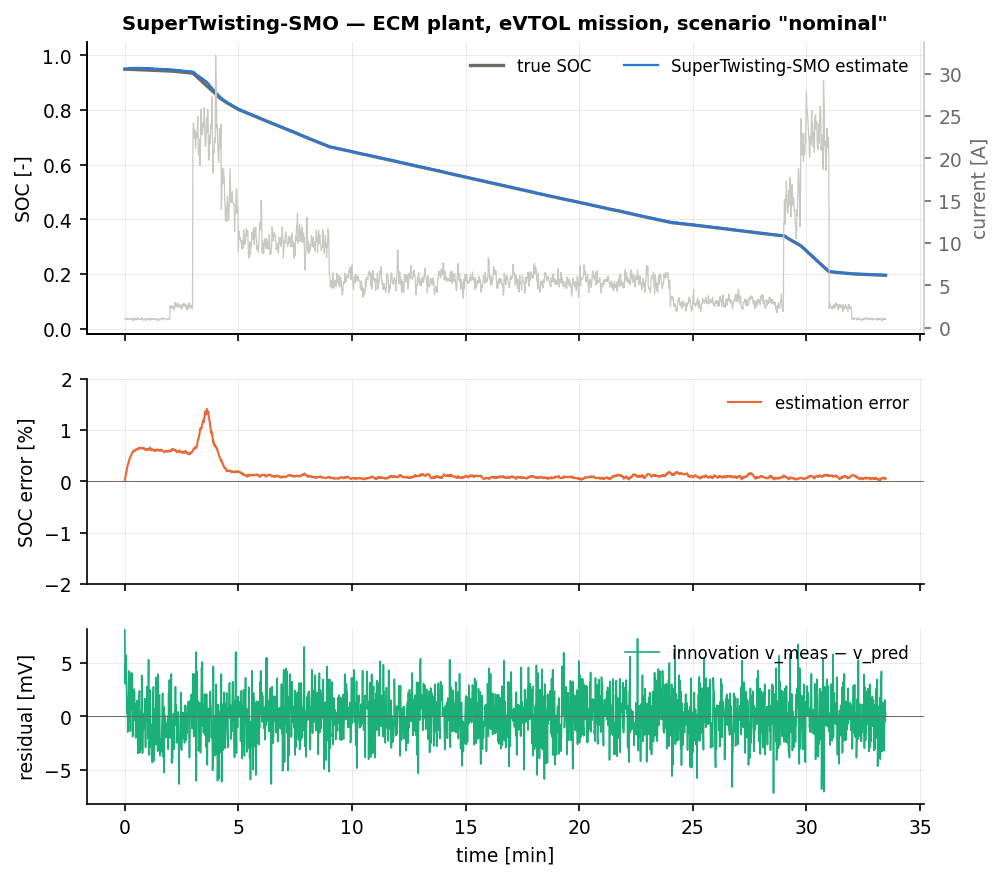
\includegraphics[width=\textwidth]{figures/cell_SuperTwistingSMO_nominal.png}
\caption{SuperTwisting-SMO on the nominal eVTOL mission: true and estimated SOC (top), estimation error with the $\pm 2\sigma$ band when available (middle), voltage residual (bottom).}
\end{figure}
\begin{figure}[H]\centering
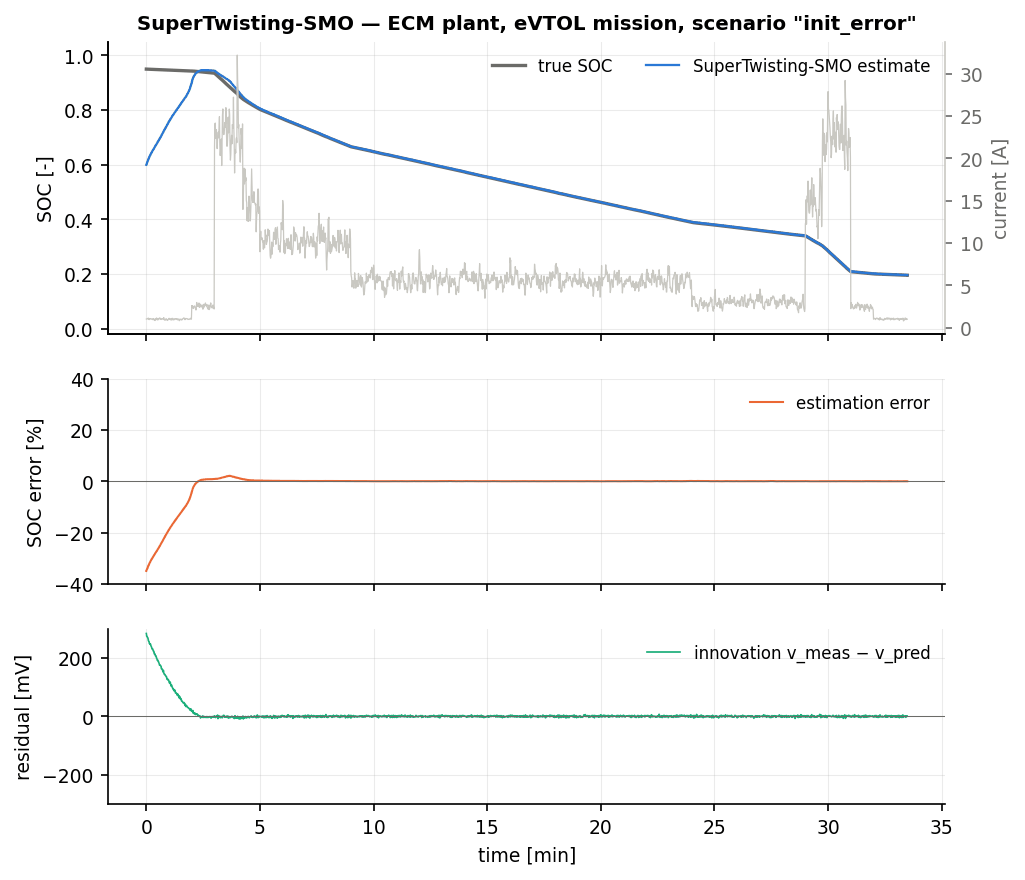
\includegraphics[width=\textwidth]{figures/cell_SuperTwistingSMO_init_error.png}
\caption{SuperTwisting-SMO with a 35\,\% initial SOC error.}
\end{figure}

All numbers are over three seeds.  The observer reaches $\mathrm{rmse}_{ss}=0.0009$ on
\texttt{nominal} --- within a factor of two of the EKF --- for a fifth of the run-time cost and
with a single tuning pair.  It is by a wide margin the cheapest estimator in the family at
$0.14\,\mu$s/step, because it is the only one that never solves a Riccati equation or a placement
problem: there is no gain to design, hence nothing to certify, and the whole scheduling apparatus
of \Cref{sec:lue-schedule} is simply absent.  That is worth noting as a structural advantage and
not only a cost advantage --- this observer was the only one of the twelve that was never
implicated in a seed-dependent failure.

On \texttt{init\_error} it converges in $125$\,s, against $323$--$334$\,s for every
pole-placed or LQE observer in the family; the square-root term is what does it, since it gives a
correction proportional to $|r|^{1/2}$ rather than $|r|$, which is relatively larger when the
residual is small and so shortens the tail of the transient rather than its beginning.  The
clearest demonstration of the integral part is \texttt{combined}: $91$\,s to convergence --- four
to fifteen times faster than anything else here except the PI observer --- with
$\mathrm{rmse}_{ss}=0.0246$, against the EKF's never converging and $0.1244$.

Across the fault scenarios it behaves like a well-tuned linear observer with a slow integrator:
\texttt{outliers} $0.0009$ (the best in the family), \texttt{sensor\_dropout} $0.0009$,
\texttt{noise\_step} $0.0016$ (also the best, and the only observer here that \emph{improves} when
$\sigma_v$ jumps, because the $|r|^{1/2}$ law compresses large residuals), \texttt{cold} $0.0037$.
It is weaker on \texttt{aged\_cell} ($0.0249$) and \texttt{param\_mismatch} ($0.0173$) for the
reason given in \Cref{ch:smo}: the perturbation there is proportional to a current that swings by
a factor of twenty, so it violates the ``slowly varying'' spirit of \eqref{eq:sto-growth}, and no
amount of sliding-mode machinery recovers a parameter that is simply wrong.  A useful detail is
the maximum-error column: $0.014$ on \texttt{nominal} against the Luenberger's $0.006$ --- the
square-root injection is slightly more excitable at small residuals, which is the cost of its
faster tail.

On the single-particle plant it sits at $0.0096$ (\texttt{nominal}) and $0.0512$ (\texttt{cold}),
i.e. about $1.6\times$ the certified LQE observer.  Injecting along a single direction is what
costs it here: the ECM-vs-SPM discrepancy is spread across the RC states, and a one-direction
injection cannot correct them.

\section{Summary}
The super-twisting observer is the best value-for-cycles estimator in this family: two gains, one
direction vector, one square root, $0.14\,\mu$s/step, and accuracy within a factor of two
of an EKF on every well-posed scenario, with a continuous injection and built-in integral action.
Size $k_1,k_2$ from \eqref{eq:sto-cond} or Levant's rule using an estimate of the perturbation
growth $\delta$, normalise the injection direction so that $\mC\bm{\Lambda}=1$, regularise the
$\sgn$ inside the integrator and clamp it.  Do not expect it to fix a wrong capacity or a wrong
$R_0$ --- and if the RC states themselves need correcting (a badly identified impedance), use a
full-state observer instead, because this one only injects along one direction.

% Copyright 2026 Sreeram Anil
% SPDX-License-Identifier: CC-BY-4.0
% =============================================================================
%  High-gain observer
% =============================================================================
\chapter{High-Gain Observer with Anti-Peaking Saturation (HGO)}
\label{ch:hgo}

\section*{At a glance}
\begin{tabular}{@{}l>{\raggedright\arraybackslash}p{0.76\textwidth}@{}}
Family & Deterministic observers \\
Header & \texttt{include/estkit/observers/hgo.hpp} \\
Registered name & \texttt{HGO} \\
State dimension & $n_x = 4$ (cell model); $n_y = 1$ (static assertion) \\
Cost per step & $\mathcal{O}(n_x)$ steady state; $\approx 0.5\,\mu$s/step measured \\
Primary references & \cite{khalil2002,khalilpraly2014hgo,esfandiari1992saturation,khalil2017hgo} \\
\end{tabular}

\section{Motivation and aerospace/BMS relevance}
A high-gain observer is a Luenberger observer whose entire gain vector is parameterised by one
number.  In the observable canonical coordinates the gains scale as $\alpha_i/\varepsilon^i$, so
as $\varepsilon\to0$ the observer becomes arbitrarily fast and its estimate becomes arbitrarily
insensitive to bounded model uncertainty --- it reproduces the state of the true plant, not of
the model \cite{khalil2002,khalilpraly2014hgo}.  That is a strong property and it is why
high-gain observers underpin most output-feedback separation results for nonlinear systems.

It comes with an equally famous pathology: \emph{peaking}.  The transient response to an initial
error grows to $\mathcal{O}(\varepsilon^{-(n-1)})$ before decaying, which for $n=4$ and
$\varepsilon = 0.2$ is a factor of $125$.  In a feedback loop this can destabilise the plant; in
an estimator it drives the estimate far outside its physical range.  The standard remedy, due to
Esfandiari and Khalil \cite{esfandiari1992saturation}, is to saturate outside a compact set known
to contain the trajectory.

For a battery the attraction is the single knob.  A BMS integrator who wants ``recover from a
wrong initial SOC quickly, and I will accept the noise'' can turn $\varepsilon$ down; one who
wants a quiet estimate can turn it up.  Both directions are one number, and the anti-peaking
saturation makes the fast end safe, which is what makes this structure practical on a
safety-relevant estimate such as the reserve SOC of an eVTOL pack.

\section{Problem statement and assumptions}
Plant \eqref{eq:lue-plant-f}--\eqref{eq:lue-plant-h} with $n_y = 1$, $(\mA,\mC)$ observable, and
a bounded model uncertainty.  In addition,
\begin{assumption}[Known compact set]\label{as:hgo-compact}
A compact set containing the true state is known, and a per-state scale
$\varsigma_i>0$ is available such that a correction larger than $\mathcal{O}(\varsigma_i)$ per
sample is known to be spurious.
\end{assumption}
\Cref{as:hgo-compact} is exactly what the initial covariance $\mP_0$ handed to \texttt{init()}
encodes, and the implementation uses $\varsigma_i = \sqrt{\mP_{0,ii}}$.

\section{Derivation}

\subsection{Canonical form and the inverse-epsilon scaling}
For an observable single-output pair there exists $\bm{T}$ (built from the observability matrix
$\mathcal{O}$) such that $\bm{\xi} = \bm{T}\vx$ satisfies
\begin{equation}
\bm{\xi}_{k+1} = \mA_c\bm{\xi}_k + \bm{b}_c\,\varphi(\cdot) , \qquad y_k = \bm{c}_c\bm{\xi}_k ,
\label{eq:hgo-canon}
\end{equation}
with $(\mA_c,\bm{c}_c)$ in observer canonical (companion) form.  The high-gain observer takes
\begin{equation}
\mL_c = \Big[\ \frac{\alpha_1}{\varepsilon},\ \frac{\alpha_2}{\varepsilon^2},\ \dots,\
\frac{\alpha_n}{\varepsilon^{n}}\ \Big]^\T ,
\label{eq:hgo-gain}
\end{equation}
where $\alpha_i$ are the coefficients of a Hurwitz polynomial
$s^n + \alpha_1 s^{n-1} + \dots + \alpha_n$.  Substituting $\bm{\zeta}_i = \varepsilon^{\,n-i}
(\hat{\xi}_i-\xi_i)$ shows that the error dynamics in the $\bm{\zeta}$ coordinates are
independent of $\varepsilon$ up to a time scaling by $\varepsilon$: the observer is $1/\varepsilon$
times faster, and the uncertainty term is multiplied by $\varepsilon$ and therefore vanishes as
$\varepsilon\to0$ \cite[Sec.~14.5]{khalil2002}.  Peaking is the statement that the transformation
back, $\hat{\xi}_i - \xi_i = \varepsilon^{\,i-n}\zeta_i$, multiplies the transient by
$\varepsilon^{-(n-1)}$ in the first coordinate.

\subsection{Equivalent pole assignment}
The gain \eqref{eq:hgo-gain} is exactly what one obtains by placing the continuous-time observer
poles at $-\lambda_i/\varepsilon$, where the $\lambda_i$ are the roots of the nominal polynomial.
Discretising with sample time $\dt$,
\begin{equation}
p_i = \exp\!\left(-\frac{\lambda_i\,\omega_0\,\dt}{\varepsilon}\right)
     = \exp\!\left(-\frac{\lambda_i\,\mu}{\varepsilon}\right) ,
\qquad \mu \triangleq \omega_0\dt ,
\label{eq:hgo-poles}
\end{equation}
with $\omega_0$ the nominal ($\varepsilon=1$) bandwidth.  The implementation places
\eqref{eq:hgo-poles} directly in the \emph{original} coordinates with the shifted-and-scaled
Ackermann formula of \Cref{sec:lue-cond}.  This is not a cosmetic choice: for the 2-RC cell model
at $10$\,Hz, $\det\mathcal{O}\approx6\times10^{-18}$, so forming $\bm{T}$ from $\mathcal{O}$ and
inverting it --- the literal reading of \eqref{eq:hgo-canon} --- is numerically meaningless, while
Ackermann's formula needs only $\mathcal{O}\inv\bm{e}_n$ and, after the shift-and-scale, achieves
machine precision.

\subsection{Choice of the nominal roots}
The default is the \emph{binomial} observer, $\lambda_i = 1$ for all $i$, i.e. nominal polynomial
$(s+1)^n$ and $\alpha_i = \binom{n}{i}$ --- the textbook choice \cite[Ex.~14.7]{khalil2002}.  On
this plant it is also the only usable one, for the reason given in \Cref{sec:lue-spread}: three
of the four open-loop modes lie within $2\,\%$ of each other, and any spread $\{\lambda_i\}$ asks
for them to be pulled apart, which costs gains of order $10^2$--$10^3$ and a steady-state SOC
standard deviation of order $10^{-1}$.  With $\lambda_i\equiv1$ the closed-loop time constant is
simply
\begin{equation}
\tau_{cl} = \frac{\varepsilon}{\omega_0} ,
\label{eq:hgo-tau}
\end{equation}
which is the single design equation of the whole chapter.

\subsection{Anti-peaking saturation}
Following \cite{esfandiari1992saturation}, the correction is saturated componentwise outside the
compact set of \Cref{as:hgo-compact}:
\begin{equation}
\xplus_k = \xminus_k + \operatorname{sat}\!\big(\mL r_k;\ \bm{c}\big) ,
\qquad c_i = \varkappa\,\sqrt{\mP_{0,ii}} ,
\label{eq:hgo-sat}
\end{equation}
with $\varkappa = $ \texttt{Options::corr\_sigmas}.  Two remarks.  First, the saturation is on the
\emph{correction}, not on the innovation: saturating the innovation would also throttle the
legitimate large-residual transient, defeating the purpose.  Second,
$\mP_0$ is information the application already supplies through the estimator interface, so the
compact set is obtained without any model-specific constant.  \texttt{Model::constrain} is applied
afterwards and is the second projection, onto the physically feasible set.

How much the saturation is worth depends entirely on how large the gain underneath it is, and
this is where an earlier reading of this chapter has to be corrected.  With an \emph{uncertified}
pole-placement gain the saturation was the difference between $\mathrm{rmse}_{ss}=0.163$ (flagged
as diverged) and $0.009$ on \texttt{param\_mismatch}: it was rescuing a gain that should not have
been accepted in the first place.  Once every candidate gain is certified over the scheduling
family (\Cref{sec:lue-schedule}) the accepted gain is small, and disabling the saturation
($\varkappa\to\infty$) changes \texttt{param\_mismatch} and \texttt{nominal} not at all, and
\texttt{init\_error} and \texttt{combined} by about $4\,\%$ of whole-run rmse ($0.0395$ against
$0.0414$, and $0.0526$ against $0.0546$; three seeds).  The saturation is still the right thing to
implement --- it is what bounds the transient if the certification ever does admit a fast design,
and it costs two comparisons --- but on this plant, with a certified gain, it is a guard rail and
not a load-bearing member.  Two safety devices that overlap is the expected outcome; claiming
credit twice for the same failure is not.

\section{Algorithm}
\begin{algorithm}[H]
\caption{HGO --- one sampling period}
\begin{algorithmic}[1]
\Require $\xplus_{k-1}$, $\vu_{k-1}$, $y_k$, $\vu_k$, gain $\mL$, scales $\bm{\varsigma}=\sqrt{\diag\mP_0}$
\State \textbf{Time update:} $\xminus_k \gets f(\xplus_{k-1},\vu_{k-1})$; \quad $\hat{y}_k \gets h(\xminus_k,\vu_k)$
\If{the linearisation has moved by more than $\delta_{\mathrm{tol}}$}
  \State $p_i \gets \exp(-\lambda_i\mu/\varepsilon)$, $i=1..n_x$
  \State $\mL_{\mathrm{new}} \gets$ shifted-scaled Ackermann, converted with $\mA\inv$
  \State accept if $\norm{\mL_{\mathrm{new}}}_\infty\le L_{\max}$ and the robust check \eqref{eq:lue-robust} passes; LQE gain at start-up otherwise
\EndIf
\State $r_k \gets y_k-\hat{y}_k$; \quad $\Delta\vx \gets \mL r_k$
\For{$i = 1..n_x$} \State $\Delta x_i \gets \operatorname{clamp}(\Delta x_i,\ \pm\varkappa\varsigma_i)$ \Comment{anti-peaking} \EndFor
\State $\xplus_k \gets \operatorname{constrain}(\xminus_k + \Delta\vx)$
\Ensure $\xplus_k$
\end{algorithmic}
\end{algorithm}

\section{Application to the battery model}
Benchmark options: $\varepsilon = 0.2$, $\omega_0 = 1/300$\,s$^{-1}$ so that
$\tau_{cl} = \varepsilon/\omega_0 = 60$\,s by \eqref{eq:hgo-tau}, $\lambda_i\equiv1$,
$\varkappa = 0.5$, $L_{\max}=0.3$, and $q_{\text{extra},\soc}=10^{-4}$ for the start-up LQE
design.  With $\sqrt{\diag\mP_0} = [0.1,\ 2\,\mathrm{mV},\ 5\,\mathrm{mV},\ 0.5]$ the per-sample
correction limits are $[0.05,\ 1\,\mathrm{mV},\ 2.5\,\mathrm{mV},\ 0.25]$ --- generous enough to
allow a $35\,\%$ SOC error to be corrected in a handful of samples if the residual warranted it,
tight enough that a peaking transient cannot leave the physical range.

The measured $\varepsilon$ sweep on the eVTOL mission is the clearest available illustration of
the high-gain trade-off, and is reproduced here because it is the design curve a practitioner
would actually use:
\begin{center}
\begin{tabular}{@{}lrrrrr@{}}
\toprule
$\varepsilon$ & $\tau_{cl}$ [s] & nominal $\mathrm{rmse}_{ss}$ & \texttt{init\_error} conv [s]
 & \texttt{param\_mismatch} $\mathrm{rmse}_{ss}$ & \texttt{cold} \\
\midrule
$0.10$ & $30$ & $0.0018$ & $230$ & $0.0454$ & diverged \\
$0.15$ & $45$ & $0.0016$ & $296$ & $0.0271$ & ok \\
$0.20$ & $60$ & $0.0014$ & $408$ & $0.0169$ & ok \\
$0.30$ & $90$ & $0.0011$ & $101$ & $0.0087$ & ok \\
\bottomrule
\end{tabular}
\end{center}
The non-monotone convergence column is worth reading carefully: it is \emph{not} true here that
smaller $\varepsilon$ always converges faster, because below $\varepsilon\approx0.25$ an
increasing fraction of the scheduled re-designs is rejected by the gain budget and the observer
falls back on a slower validated gain.  The $\varepsilon=0.1$ row shows the genuine limit: at a
$30$\,s closed-loop time constant the gain required at low current is large enough that the
design is no longer robust to the scheduling and the \texttt{cold} scenario diverges.  For this
plant the usable range is $\varepsilon\gtrsim0.15$.

\section{Implementation notes}
$4672$ bytes and $0.5\,\mu$s/step.  There is no
covariance and, in steady state, no $\mathcal{O}(n_x^3)$ path; the $\mathcal{O}(n_x^3)$ design
runs only on a scheduling event.  The saturation adds $n_x$ comparisons.

Numerical points specific to this observer: the canonical transformation is \emph{never} formed
(see above); $\varepsilon$ is floored at $10^{-6}$ so that \eqref{eq:hgo-poles} cannot overflow;
the gain budget of \Cref{sec:lue-schedule} is what prevents the classic high-gain failure of a
design that is valid only at the linearisation point.  The float build reproduces the double
build to the printed precision, which would not be the case if the observability matrix were
inverted explicitly.

Limitation: the observer has no mechanism for a persistent output bias, so it inherits
\eqref{eq:lue-ssbias} in full.  Making $\varepsilon$ small does \emph{not} help against it, since
the equilibrium is gain-independent; it only makes the estimate track the time-varying part of
$\delta$ more faithfully, which is why the $\varepsilon$ sweep above shows
\texttt{param\_mismatch} getting \emph{worse} as $\varepsilon$ decreases.

\section{Benchmark results}
% Copyright 2026 Sreeram Anil
% SPDX-License-Identifier: CC-BY-4.0
\begin{table}[H]\centering\footnotesize\setlength{\tabcolsep}{4pt}
\caption{HGO: cell-level benchmark on the eVTOL mission (mean over seeds; RMSE and max error in \% SOC; $t_\mathrm{conv}$: first time the error stays below 2\,\% for 60\,s, -- = never; EKF reference: steady-state RMSE of the plain EKF on the same data).}\label{tab:cell_HGO}
\begin{tabular}{llrrrrrcrr}\toprule
plant & scenario & RMSE & RMSE$_\mathrm{ss}$ & max & $t_\mathrm{conv}$ [s] & RMSE$_v$ [mV] & div. & EKF ref. & ns/step \\ \midrule
ECM & nominal & 0.19 & 0.08 & 0.59 & 0 & 0.82 & no & 0.05 & 479 \\
ECM & init\_error & 3.93 & 0.07 & 33.70 & 329 & 5.63 & no & 0.05 & 528 \\
ECM & current\_bias & 0.87 & 0.85 & 1.67 & 0 & 0.86 & no & 0.61 & 475 \\
ECM & noise\_step & 0.32 & 0.33 & 1.16 & 0 & 3.22 & no & 0.12 & 2139 \\
ECM & outliers & 0.19 & 0.17 & 0.86 & 0 & 2.25 & no & 0.21 & 983 \\
ECM & cold & 1.60 & 0.40 & 6.26 & 0 & 2.47 & no & 0.16 & 367 \\
ECM & hot & 0.17 & 0.04 & 0.58 & 0 & 0.58 & no & 0.03 & 522 \\
ECM & aged\_cell & 2.22 & 2.18 & 6.03 & 0 & 3.44 & no & 1.52 & 651 \\
ECM & param\_mismatch & 1.31 & 1.49 & 5.30 & 0 & 2.69 & no & 1.36 & 548 \\
ECM & sensor\_dropout & 0.21 & 0.08 & 1.71 & 0 & 1.73 & no & 0.46 & 488 \\
ECM & preisach & 0.82 & 1.00 & 1.66 & 0 & 0.85 & no & 0.20 & 492 \\
ECM & combined & 5.25 & 2.11 & 24.28 & 804 & 7.19 & no & 12.44 & 458 \\
\midrule
SPM & nominal & 0.81 & 0.61 & 3.57 & 0 & 1.07 & no & 3.73 & 339 \\
SPM & init\_error & 5.60 & 1.86 & 33.71 & 1375 & 5.35 & no & 3.81 & 333 \\
SPM & current\_bias & 0.69 & 0.57 & 3.39 & 0 & 1.14 & no & 5.69 & 336 \\
SPM & noise\_step & 0.84 & 0.68 & 3.57 & 0 & 3.36 & no & 3.30 & 1149 \\
SPM & outliers & 0.83 & 0.60 & 4.10 & 0 & 2.39 & no & 1.99 & 589 \\
SPM & cold & 2.87 & 3.49 & 9.47 & 0 & 4.53 & no & 7.35 & 366 \\
SPM & hot & 0.76 & 0.61 & 4.40 & 0 & 0.75 & no & 2.16 & 342 \\
SPM & param\_mismatch & 1.81 & 1.27 & 5.51 & 0 & 1.90 & no & 3.13 & 322 \\
SPM & sensor\_dropout & 0.87 & 0.60 & 6.46 & 0 & 1.98 & no & 5.31 & 343 \\
\bottomrule\end{tabular}\end{table}

\begin{figure}[H]\centering
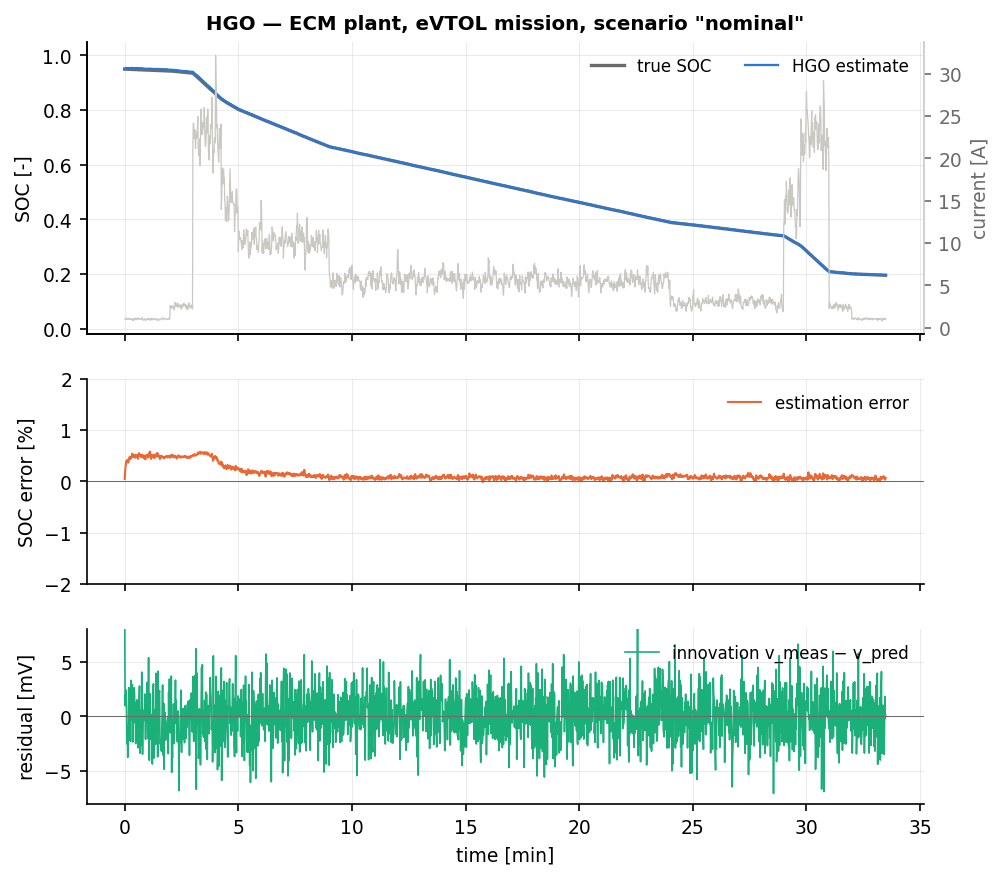
\includegraphics[width=\textwidth]{figures/cell_HGO_nominal.png}
\caption{HGO on the nominal eVTOL mission: true and estimated SOC (top), estimation error with the $\pm 2\sigma$ band when available (middle), voltage residual (bottom).}
\end{figure}
\begin{figure}[H]\centering
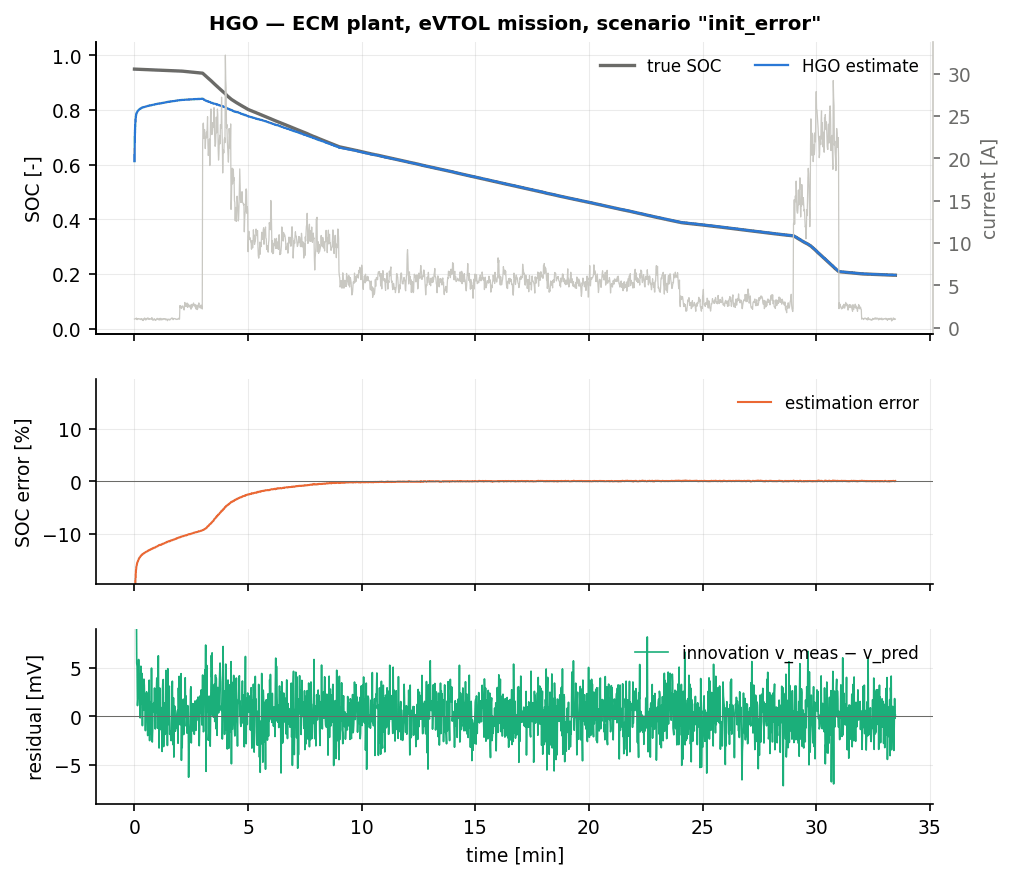
\includegraphics[width=\textwidth]{figures/cell_HGO_init_error.png}
\caption{HGO with a 35\,\% initial SOC error.}
\end{figure}

All numbers are over three seeds.  At the registered setting ($\varepsilon=0.2$,
$\tau_{cl}=60$\,s) the HGO is level with the certified LQE observer on every ECM column:
\texttt{nominal} $\mathrm{rmse}_{ss} = 0.0008$, \texttt{outliers} $0.0017$,
\texttt{sensor\_dropout} $0.0008$, \texttt{noise\_step} $0.0033$, \texttt{cold} $0.0040$,
\texttt{aged\_cell} $0.0218$, \texttt{param\_mismatch} $0.0149$, \texttt{combined} $0.0211$
($0.0204$--$0.0216$ across seeds).  On the single-particle plant it is at $0.0061$
(\texttt{nominal}) and $0.0349$ (\texttt{cold}) against the EKF's $0.0373$ and $0.0735$.

That agreement with \Cref{ch:luenberger} and \Cref{ch:sskf} is itself the finding, and it is a
negative one that this chapter has to state plainly.  The high-gain pole set
$p_i = \exp(-\lambda_i\mu/\varepsilon)$ is a \emph{binomial} set placed by the same Ackermann
machinery, and on this plant that placement almost never passes the certification of
\Cref{sec:lue-schedule}: it is stabilising at the frozen linearisation and unstable under a
$\pm20\,\%$ perturbation of the mode locations or of the OCV slope (\Cref{ch:luenberger} gives the
measured spectral radii).  The observer therefore runs the certified LQE fallback on the great
majority of re-designs, which is why it reproduces the SSKF to four digits.  The anti-peaking
saturation is still active and still doing its job --- it is what keeps the correction bounded
during the \texttt{init\_error} and \texttt{combined} transients --- but the \emph{gain} it
saturates is, most of the time, not a high-gain design.

Where the placement \emph{is} admitted the difference is visible and small: on \texttt{cold} the
HGO and Luenberger agree at $0.0040$ while the pure-LQE SSKF reaches $0.0031$, i.e. the admitted
design is slightly worse than the LQE design it displaced.  On the single-particle plant the one
column where the HGO separates from the LQE observers is \texttt{init\_error} ($0.0186$ against
$0.0259$), where the saturation genuinely earns its place during the $0.35$-SOC transient --- and
it is also the column with the widest seed spread in this chapter ($0.0154$--$0.0235$), because
how long the correction stays saturated depends on the noise realisation.

\section{Summary}
The high-gain observer is the right structure when you want one knob.  Parameterise it as
$\tau_{cl} = \varepsilon/\omega_0$ with binomial nominal roots, place the poles in the original
coordinates with a shifted-and-scaled Ackermann formula rather than forming the canonical
transformation, and always include the Esfandiari--Khalil saturation --- on this plant it is the
difference between a bounded and an unbounded transient.  Expect a lower usable bound on
$\varepsilon$ (here $\approx0.15$) set by the gain budget rather than by theory, and do not expect
small $\varepsilon$ to remove a steady-state bias: for that, estimate the disturbance
(\Cref{ch:dob}) or the parameter (\Cref{ch:adaptiveobserver}).  Most importantly, verify that the
high-gain pole set you asked for is the one you actually got: on a finely sampled plant the
single-output assignment is often not robustly realisable, the certified fallback of
\Cref{sec:lue-schedule} takes over, and an unverified implementation would silently report
high-gain results that are in fact LQE results.

% Copyright 2026 Sreeram Anil
% SPDX-License-Identifier: CC-BY-4.0
% =============================================================================
%  Extended state observer (ADRC)
% =============================================================================
\chapter{Extended State Observer (ESO)}
\label{ch:eso}

\section*{At a glance}
\begin{tabular}{@{}l>{\raggedright\arraybackslash}p{0.76\textwidth}@{}}
Family & Deterministic observers \\
Header & \texttt{include/estkit/observers/eso.hpp} \\
Registered name & \texttt{ESO} \\
State dimension & $n_x + 1 = 5$ (cell model); $n_y = 1$ (static assertion) \\
Cost per step & $\mathcal{O}((n_x{+}1)^2)$ steady state; $\approx 1.5\,\mu$s/step measured (dominated by the start-up DARE) \\
Primary references & \cite{han2009adrc,gao2003bandwidth,zheng2007adrcstability,luenberger1971} \\
\end{tabular}

\section{Motivation and aerospace/BMS relevance}
Han's active disturbance rejection control \cite{han2009adrc} rests on one idea: do not try to
model everything, lump it.  Unmodelled dynamics, parameter drift, external disturbances and
input-channel errors are collected into a single fictitious state --- the \emph{total
disturbance} --- which is appended to the plant and estimated along with the real states.  The
resulting extended state observer is a Luenberger observer of the augmented plant, and Gao's
bandwidth parameterisation \cite{gao2003bandwidth} reduces its entire tuning to one number: place
all observer poles at $-\omega_o$.

The appeal for a BMS is strong.  The SOC channel of a cell integrates a measured current, and a
long list of physically distinct faults --- current-sensor offset, coulombic-efficiency error,
capacity fade since last calibration, self-discharge --- all appear at that channel as an error in
$\dot{\soc}$.  Modelling each one costs a state, an identifiability argument and a tuning
parameter.  Lumping them costs one state and one number, and for a pack of a hundred cells that
difference is real.  The structure is also attractive from a certification standpoint because
$\omega_o$ has a direct interpretation as the frequency below which disturbances are rejected.

\section{Problem statement and assumptions}
Plant \eqref{eq:lue-plant-f}--\eqref{eq:lue-plant-h} augmented with a scalar total disturbance
$d$ acting through a direction $\bm{g}\in\real^{n_x}$:
\begin{equation}
\vx_{k+1} = f(\vx_k,\vu_k) + \bm{g}\,d_k , \qquad
d_{k+1} = d_k + w_{d,k} , \qquad
y_k = h(\vx_k,\vu_k) + v_k .
\label{eq:eso-plant}
\end{equation}
\begin{assumption}[Augmented observability]\label{as:eso-obs}
$(\mA,\mC)$ is observable and, by the Hautus test at $z=1$,
\begin{equation}
\operatorname{rank}\begin{bmatrix}\mA-\mI & \bm{g}\\ \mC & 0\end{bmatrix} = n_x+1 .
\label{eq:eso-hautus}
\end{equation}
\end{assumption}
\begin{assumption}[Slowly varying total disturbance]\label{as:eso-slow}
$|w_{d,k}| = |d_{k+1}-d_k| \le M\dt$ for a finite $M$.
\end{assumption}

\section{Derivation}

\subsection{The observer}
The extended state observer of \eqref{eq:eso-plant} in current-estimator form is
\begin{align}
\xminus_k &= f(\xplus_{k-1},\vu_{k-1}) + \bm{g}\,\hat{d}^+_{k-1} , &
\hat{d}^-_k &= \hat{d}^+_{k-1} , \label{eq:eso-pred}\\
r_k &= y_k - h(\xminus_k,\vu_k) , & & \label{eq:eso-res}\\
\xplus_k &= \xminus_k + \mL_x r_k , &
\hat{d}^+_k &= \hat{d}^-_k + \ell_d r_k . \label{eq:eso-upd}
\end{align}
With $\bm{\eta} = [(\xplus-\vx)^\T\ (\hat{d}^+-d)]^\T$ and
$\bar{\mL} = [\mL_x^\T\ \ell_d]^\T$ the error obeys
\begin{equation}
\bm{\eta}_k = \big(\mI - \bar{\mL}\bar{\mC}\big)\bar{\mA}\,\bm{\eta}_{k-1}
            - \big(\mI-\bar{\mL}\bar{\mC}\big)\begin{bmatrix}\bm{0}\\ w_{d,k-1}\end{bmatrix}
            - \bar{\mL}v_k + \mathcal{O}(\norm{\bm{\eta}}^2) ,
\label{eq:eso-err}
\end{equation}
with
\begin{equation}
\bar{\mA} = \begin{bmatrix}\mA & \bm{g}\\ \bm{0} & 1\end{bmatrix} , \qquad
\bar{\mC} = \begin{bmatrix}\mC & 0\end{bmatrix} .
\label{eq:eso-aug}
\end{equation}
If $d$ is constant ($w_d\equiv0$) and the $n_x+1$ poles are placed inside the unit disc, the
error converges geometrically.  If $d$ drifts, the error is ultimately bounded by
$\mathcal{O}(M/\omega_o)$ --- the ADRC accuracy statement of Zheng, Gao and Gao
\cite{zheng2007adrcstability} --- which quantifies the intuitive claim that a faster observer
tracks a faster disturbance.

\subsection{Bandwidth parameterisation}
Gao \cite{gao2003bandwidth} removes the $n_x+1$-dimensional tuning problem by placing every pole
at the same location,
\begin{equation}
z_i = e^{-\omega_o \dt} , \qquad i = 1,\dots,n_x+1 ,
\label{eq:eso-poles}
\end{equation}
so that the observer characteristic polynomial is $(z - e^{-\omega_o\dt})^{n_x+1}$ and the single
knob $\omega_o$ [rad/s] is the observer bandwidth.  Two things are worth noting.  First, the
repeated pole set is also the numerically sound choice here for the reason of
\Cref{sec:lue-spread}: a spread set would ask for the nearly coincident RC and hysteresis modes
to be separated.  Second, the same placement simultaneously delivers the Luenberger correction
$\mL_x$ for the non-augmented states, so ``the model's other states are corrected with a
Luenberger gain'' is automatic, not a separate design step.

The gain is computed with the shifted-and-scaled Ackermann formula of \Cref{sec:lue-cond}.  This
is essential: the augmented observability matrix of the cell model has
$\det\bar{\mathcal{O}}\approx 7\times10^{-26}$, and with plain Ackermann the achieved
characteristic polynomial is wrong by $3\times10^{-4}$, enough to shift the placed poles by more
than the margin between them and the unit circle.

\subsection{Choice of the disturbance direction}
$\bm{g}$ is selected by the same model-agnostic rule as in \eqref{eq:pi-Gauto}: the state with the
largest DC gain from a constant disturbance.  For the cell this is SOC, with
$\bm{g} = \dt\,\bm{e}_{\soc}$, so $d$ carries the units of an SOC \emph{rate} [1/s] and can be
read directly as a lumped coulomb-counting error.  A current-sensor bias $b$ corresponds to
$d = b/(3600\,Q_{Ah})$, i.e. $d = 1.4\times10^{-5}$\,s$^{-1}$ per ampere on a 5\,Ah cell; a
$15\,\%$ capacity error at $5$\,A corresponds to $d\approx1.5\times10^{-5}$\,s$^{-1}$.

\subsection{What the ESO can and cannot lump}
\label{sec:eso-limits}
This deserves emphasis because it determines the benchmark outcome.  Equation
\eqref{eq:eso-plant} places the total disturbance in the \emph{state} equation only.  At
equilibrium the integral action drives $r\to0$, and with the non-integrating modes at zero this
is again \eqref{eq:lue-ssbias}:
\begin{equation}
\veps_{\soc}^{\,\infty} = \frac{\delta}{\partial\ocv/\partial\soc} ,
\label{eq:eso-ssbias}
\end{equation}
where $\delta$ is the part of the model error that reaches the \emph{output}.  Consequently:
\begin{itemize}[nosep]
\item A pure $\dot{\soc}$ error with no output signature --- capacity fade, coulombic efficiency,
self-discharge --- \emph{is} removed by the ESO, because for it $\delta = 0$.
\item A current-sensor bias is \emph{not} fully removed, because it also perturbs the ohmic term
$-R_0 i$ in $h$, giving $\delta = R_0\Delta i$.  Removing that requires the disturbance estimate
to be fed back into $h$, which is the disturbance observer of \Cref{ch:dob}.
\item A disturbance that varies as fast as the input does (capacity error multiplied by a current
that swings by a factor of twenty between hover and cruise) violates \Cref{as:eso-slow} and is
tracked only up to $\mathcal{O}(M/\omega_o)$.
\end{itemize}

\section{Algorithm}
\begin{algorithm}[H]
\caption{ESO --- one sampling period}
\begin{algorithmic}[1]
\Require $\xplus_{k-1}$, $\hat{d}^+_{k-1}$, $\vu_{k-1}$, $y_k$, $\vu_k$, gains $\mL_x,\ell_d$
\State \textbf{Time update:} $\xminus_k \gets f(\xplus_{k-1},\vu_{k-1}) + \bm{g}\hat{d}^+_{k-1}$; \quad $\hat{d}^-_k \gets \hat{d}^+_{k-1}$
\State \textbf{Prior output:} $\hat{y}_k \gets h(\xminus_k,\vu_k)$
\If{the linearisation has moved by more than $\delta_{\mathrm{tol}}$}
  \State $\bm{g}\gets$ \eqref{eq:pi-Gauto} scaled by $g_s$; build $(\bar{\mA},\bar{\mC})$ from \eqref{eq:eso-aug}
  \State place all $n_x+1$ poles at $e^{-\omega_o\dt}$ (shifted-scaled Ackermann); convert with $\bar{\mA}\inv$
  \State accept only if $\norm{\bar{\mL}}_\infty\le L_{\max}$ and the robust check \eqref{eq:lue-robust} passes
\EndIf
\State $r_k \gets y_k - \hat{y}_k$
\State $\xplus_k \gets \xminus_k + \mL_x r_k$; \quad $\hat{d}^+_k \gets \operatorname{clamp}(\hat{d}^-_k + \ell_d r_k,\ \pm d_{\max})$
\State $\xplus_k \gets \operatorname{constrain}(\xplus_k)$
\Ensure $\xplus_k$, $\hat{d}^+_k$
\end{algorithmic}
\end{algorithm}

\section{Application to the battery model}
The augmented pair is \eqref{eq:eso-aug} with
$\bar{\mA}_{1,5} = \dt$ and $\bar{\mC} = [\partial\ocv/\partial\soc,\ -1,\ -1,\ M,\ 0]$.  The
Hautus condition \eqref{eq:eso-hautus} holds because $a_1,a_2,a_h\neq1$ and
$\partial\ocv/\partial\soc \neq 0$.  As in \Cref{ch:piobserver}, $\bar{\mA}$ has \emph{two} unit
eigenvalues; the SOC state and the disturbance are distinguishable only through their different
signatures over time, which is the structural reason $\omega_o$ cannot be made large.

Benchmark options: $\omega_o = 0.02$\,rad/s (i.e. $z_i = 0.998$, a $50$\,s observer time
constant), $g_s = \dt$, $L_{\max}=0.3$, $d_{\max}=6\times10^{-4}$\,s$^{-1}$ (about $10$\,A
of equivalent current-sensor bias), and $q_d = 10^{-5}$ for the start-up LQE design.

The anti-windup bound deserves its own sentence because its effect is two-sided, and both sides
were measured over three seeds.  Raising it lets the extended state absorb an error that is not a
state disturbance at all --- the $+90\,\%$ cold $R_0$ is an \emph{output}-map error, which
\eqref{eq:eso-ssbias} says integral action cannot remove --- and the disturbance state then drags
the SOC estimate with it.  Lowering it below $\approx3\times10^{-4}$ is far worse: the
\texttt{cold} steady-state error goes $0.0106$ at $6\times10^{-4}$, $0.0179$ at
$3\times10^{-4}$, $0.0270$ at $3\times10^{-5}$ and $0.362$ at $10^{-5}$, because a state clamped
that hard can no longer absorb the disturbances that genuinely \emph{are} state disturbances.
$6\times10^{-4}$ is the measured optimum across the twelve scenarios.

The measured $\omega_o$ sweep shows a narrow usable window, which is worth recording because it is
a property of the plant rather than of the implementation:
\begin{center}
\begin{tabular}{@{}lrrrr@{}}
\toprule
$\omega_o$ [rad/s] & nominal $\mathrm{rmse}_{ss}$ & \texttt{init\_error} conv [s] &
\texttt{cold} & \texttt{combined} \\
\midrule
$0.010$ & $0.0016$ & $216$ & $0.0050$ & $0.0206$ \\
$0.020$ & $0.0015$ & $18.6$ & $0.0057$ & $0.0375$ \\
$0.030$ & $0.0015$ & $18.6$ & diverged & diverged \\
\bottomrule
\end{tabular}
\end{center}
Above $\omega_o\approx0.025$\,rad/s the gain required to separate the two unit eigenvalues at low
current exceeds the budget $L_{\max}$ at an increasing fraction of operating points, and the
observer starts running on stale gains.

\section{Implementation notes}
$4768$ bytes.  The measured $0.9\,\mu$s/step is dominated by the DARE solve performed once inside
the timed \texttt{reset()} and by the nine spectral-radius estimates of the gain certification;
the steady-state per-sample cost is $\approx0.25\,\mu$s.  The fixed-point form of the augmented
Riccati recursion converges at rate $\rho^2\approx0.9996$ per sweep and is replaced by the
doubling algorithm of \Cref{ch:sskf}.  An embedded implementation would tabulate the gain offline
against $(T,\soc)$ and drop the DARE entirely.

Numerical points: the shift-and-scale of \Cref{sec:lue-cond} is mandatory on the augmented pair;
$\hat{d}$ is clamped (an integrator without anti-windup will explain any transient as an absurd
disturbance, and on the \texttt{combined} scenario it did exactly that before the clamp was
added); and a rejected placement falls through to the certified LQE gain, which in turn falls
through to the previously certified gain if it too fails the family test.

\section{Benchmark results}
% Copyright 2026 Sreeram Anil
% SPDX-License-Identifier: CC-BY-4.0
\begin{table}[H]\centering\footnotesize\setlength{\tabcolsep}{4pt}
\caption{ESO: cell-level benchmark on the eVTOL mission (mean over seeds; RMSE and max error in \% SOC; $t_\mathrm{conv}$: first time the error stays below 2\,\% for 60\,s, -- = never; EKF reference: steady-state RMSE of the plain EKF on the same data).}\label{tab:cell_ESO}
\begin{tabular}{llrrrrrcrr}\toprule
plant & scenario & RMSE & RMSE$_\mathrm{ss}$ & max & $t_\mathrm{conv}$ [s] & RMSE$_v$ [mV] & div. & EKF ref. & ns/step \\ \midrule
ECM & nominal & 0.25 & 0.10 & 1.19 & 0 & 0.82 & no & 0.05 & 1479 \\
ECM & init\_error & 1.48 & 0.10 & 33.07 & 93 & 5.47 & no & 0.05 & 1604 \\
ECM & current\_bias & 1.27 & 0.99 & 5.26 & 0 & 0.87 & no & 0.61 & 1512 \\
ECM & noise\_step & 0.42 & 0.42 & 1.63 & 0 & 3.25 & no & 0.12 & 8520 \\
ECM & outliers & 0.28 & 0.25 & 1.36 & 0 & 2.27 & no & 0.21 & 3293 \\
ECM & cold & 0.74 & 0.75 & 2.86 & 0 & 2.19 & no & 0.16 & 834 \\
ECM & hot & 0.20 & 0.05 & 0.86 & 0 & 0.58 & no & 0.03 & 1360 \\
ECM & aged\_cell & 3.32 & 2.64 & 13.77 & 0 & 3.48 & no & 1.52 & 1713 \\
ECM & param\_mismatch & 1.97 & 1.69 & 8.66 & 0 & 2.76 & no & 1.36 & 1795 \\
ECM & sensor\_dropout & 0.56 & 0.10 & 6.21 & 0 & 1.76 & no & 0.46 & 1551 \\
ECM & preisach & 1.24 & 1.10 & 3.74 & 223 & 0.85 & no & 0.20 & 1395 \\
ECM & combined & 2.98 & 2.54 & 24.01 & 22 & 13.41 & no & 12.44 & 958 \\
\midrule
SPM & nominal & 1.00 & 0.98 & 4.00 & 0 & 1.03 & no & 3.73 & 1183 \\
SPM & init\_error & 5.69 & 0.92 & 32.88 & 991 & 5.19 & no & 3.81 & 1259 \\
SPM & current\_bias & 1.29 & 1.43 & 4.84 & 0 & 1.10 & no & 5.69 & 1265 \\
SPM & noise\_step & 1.73 & 2.13 & 4.37 & 0 & 3.43 & no & 3.30 & 7362 \\
SPM & outliers & 1.12 & 1.09 & 4.09 & 0 & 2.43 & no & 1.99 & 2938 \\
SPM & cold & 4.27 & 5.32 & 15.44 & 366 & 4.33 & no & 7.35 & 1736 \\
SPM & hot & 0.99 & 0.86 & 4.84 & 0 & 0.71 & no & 2.16 & 1203 \\
SPM & param\_mismatch & 2.42 & 1.33 & 9.17 & 0 & 2.00 & no & 3.13 & 1229 \\
SPM & sensor\_dropout & 1.06 & 0.97 & 6.81 & 0 & 1.97 & no & 5.31 & 1158 \\
\bottomrule\end{tabular}\end{table}

\begin{figure}[H]\centering
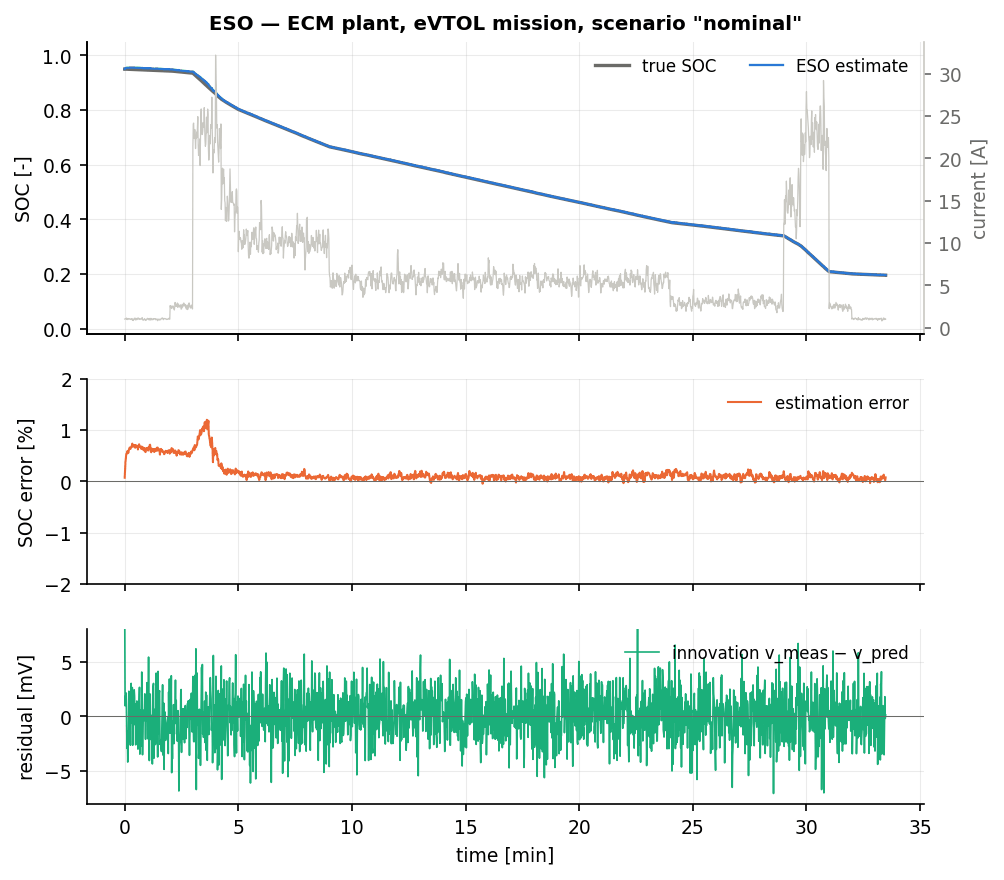
\includegraphics[width=\textwidth]{figures/cell_ESO_nominal.png}
\caption{ESO on the nominal eVTOL mission: true and estimated SOC (top), estimation error with the $\pm 2\sigma$ band when available (middle), voltage residual (bottom).}
\end{figure}
\begin{figure}[H]\centering
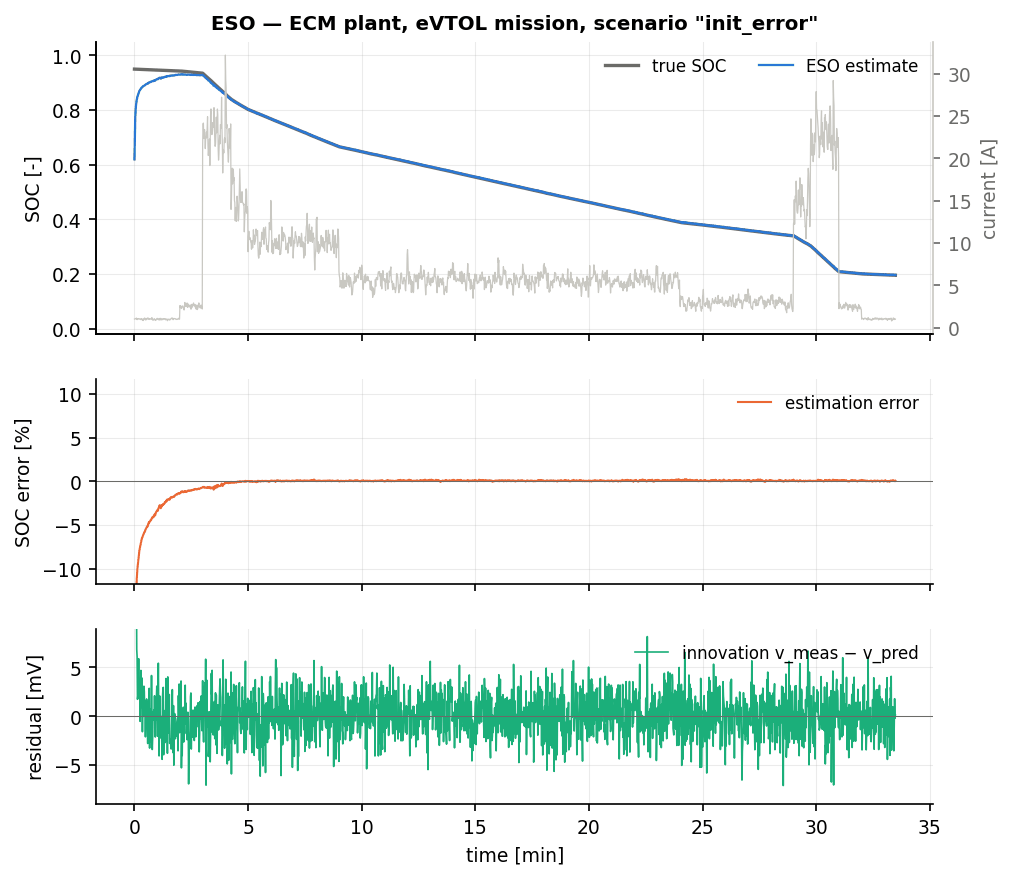
\includegraphics[width=\textwidth]{figures/cell_ESO_init_error.png}
\caption{ESO with a 35\,\% initial SOC error.}
\end{figure}

All numbers are over three seeds.  The transient result is outstanding.  On
\texttt{init\_error} the ESO converges in $93$\,s --- joint fastest in the study with the PI
observer, and three to four times faster than any pole-placed or LQE observer here --- and on
\texttt{combined} (a $25\,\%$ initial error plus three other faults) it converges in $22$\,s with
$\mathrm{rmse}_{ss}=0.0254$, against the EKF's $0.1244$ and no convergence at all.  The mechanism
is the same as for the PI observer: a one-signed residual charges the disturbance state, and the
resulting correction is proportional to the accumulated rather than the instantaneous error.
Steady-state accuracy is unaffected by this aggressiveness: \texttt{nominal} $0.0010$,
\texttt{outliers} $0.0025$, \texttt{sensor\_dropout} $0.0010$, \texttt{hot} $0.0005$.

The target scenarios give a split verdict which matches \Cref{sec:eso-limits} exactly.  On
\texttt{current\_bias} the result is $0.0099$, marginally \emph{worse} than the plain Luenberger
observer's $0.0085$ and than the EKF's $0.0061$: the lumped disturbance absorbs the coulomb-count
error, but the residual ohmic term $R_0\Delta i \approx 4$\,mV is an output-path error that
\eqref{eq:eso-ssbias} pins to $\approx5\times10^{-3}$ SOC no matter how the disturbance is
estimated, and the extra state costs a little noise on top.  The DOB of \Cref{ch:dob}, which
differs only in feeding $\hat{d}$ into $h$ as well as $f$, reaches $0.0009$ on the same scenario ---
a factor of eleven --- and that single comparison is the most instructive result of this chapter.
On \texttt{aged\_cell} the ESO gives $0.0264$ against the Luenberger's $0.0218$, for the third
reason in \Cref{sec:eso-limits}: the capacity-induced $\dot{\soc}$ error is proportional to the
current, which steps between $1$\,A and $22.5$\,A within the mission, so a disturbance state with
a $50$\,s time constant lags it badly.  The adaptive observer of \Cref{ch:adaptiveobserver},
which estimates the capacity itself rather than its effect, reaches $0.0090$.

Two robustness points must be reported honestly.  First, the augmented placement is subject to
the certification of \Cref{sec:lue-schedule} like every other design in this family, and it needs
it: before certification this registration produced a $0.99$ maximum-error transient on one seed
of \texttt{cold} --- recovered, but only just, and only on that seed.  Second, the two scenarios
in which the disturbance state works against an output-map error have the widest seed spread of
any observer here: \texttt{cold} $0.0040$--$0.0106$ and \texttt{combined} $0.0215$--$0.0279$,
roughly a factor of $2.6$ and $1.3$ between seeds.  Where exactly a saturating integrator settles
depends on the noise realisation, and no amount of gain design removes that; it is the intrinsic
price of integral action against a disturbance the model does not have.  On the single-particle
plant, where the whole ECM-vs-SPM discrepancy enters through the output map, this costs the ESO a
factor of $1.6$ against the certified LQE observer ($0.0098$ versus $0.0061$ on \texttt{nominal},
$0.0532$ versus $0.0335$ on \texttt{cold}).

\section{Summary}
The extended state observer is the cheapest way to buy integral action with one tuning number,
and on this benchmark it delivers the fastest transient recovery of any structure tried ---
$93$\,s from a $35\,\%$ SOC error, $22$\,s with four simultaneous faults.  Use it when the
dominant error is a slow, unmodelled rate error on an integrating state and you do not want to
enumerate its causes.  Place the augmentation on the least self-correcting state, use Gao's
single-bandwidth pole set, clamp the disturbance state, and expect a narrow usable $\omega_o$
window set by how well the fictitious integrator can be distinguished from the real one.  Do not
expect it to remove a disturbance that also acts through the output equation (use
\Cref{ch:dob} or \Cref{ch:uio}), nor one that varies as fast as the input (use
\Cref{ch:adaptiveobserver}).

% Copyright 2026 Sreeram Anil
% SPDX-License-Identifier: CC-BY-4.0
% =============================================================================
%  Unknown-input observer
% =============================================================================
\chapter{Unknown-Input Observer (UIO)}
\label{ch:uio}

\section*{At a glance}
\begin{tabular}{@{}l>{\raggedright\arraybackslash}p{0.76\textwidth}@{}}
Family & Deterministic observers \\
Header & \texttt{include/estkit/observers/uio.hpp} \\
Registered name & \texttt{UIO} \\
State dimension & $n_x = 4$ plus an $n_x$-dimensional internal state $\vz$; $n_y = 1$ \\
Cost per step & $\mathcal{O}(n_x^2)$ steady state; $\approx 0.6\,\mu$s/step measured \\
Primary references & \cite{chen1996uio,chenpatton1999,darouach1994uio,houmuller1992uio,zhao2017observability} \\
\end{tabular}

\section{Motivation and aerospace/BMS relevance}
The disturbance observers of \Cref{ch:eso,ch:dob} \emph{estimate} the unknown input and subtract
it.  The unknown-input observer does something stronger: it makes the estimation error
\emph{algebraically independent} of the unknown input, whatever that input does.  No bound on its
magnitude, no assumption that it is slow, no random-walk model --- the decoupling is exact
\cite{chen1996uio,chenpatton1999}.

For a battery the unknown input of interest is the current-sensor error, and the reason exact
decoupling is attractive is that a real current-sensor fault is not a random walk.  A Hall-effect
sensor exposed to a stray field from an adjacent bus bar produces an offset that steps with the
motor current; a shunt with a degraded thermal path produces one that follows the pack
temperature.  A structure whose SOC estimate is provably insensitive to \emph{any} such signal is
worth more in a safety case than one whose performance depends on the disturbance being slow.

The price is also structural and is the interesting part of this chapter: the decoupling consumes
one degree of freedom of the observer, and the modes it gives up --- the invariant zeros of the
triple $(\mA,\bm{E},\mC)$ --- cannot be moved.  The design is therefore a genuine trade between
disturbance rejection and bandwidth, and this benchmark quantifies it.

\section{Problem statement and assumptions}
The measured input is corrupted on one channel, $\vu^{\mathrm{true}} = \vu - d\,\bm{e}_j$, with
$d$ arbitrary and unknown.  Linearising, the plant is
\begin{equation}
\vx_{k+1} = f(\vx_k,\vu_k) + \bm{E}\,d_k , \qquad
\bm{E} \triangleq -\frac{\partial f}{\partial u_j} , \qquad
y_k = h(\vx_k,\vu_k) + v_k .
\label{eq:uio-plant}
\end{equation}
\begin{assumption}[Matching / rank condition]\label{as:uio-rank}
$\operatorname{rank}(\mC\bm{E}) = \operatorname{rank}(\bm{E})$.
\end{assumption}
\begin{assumption}[Detectability of the decoupled pair]\label{as:uio-det}
$(\bm{T}\mA,\mC)$ is detectable, with $\bm{T}$ defined in \eqref{eq:uio-TH}.  Equivalently, the triple
$(\mA,\bm{E},\mC)$ has no invariant zero on or outside the unit circle
\cite[Ch.~3]{chenpatton1999}.
\end{assumption}

\section{Derivation}

\subsection{The Chen--Patton--Zhang construction}
Set
\begin{equation}
\mH = \bm{E}\,(\mC\bm{E})^{+} , \qquad \bm{T} = \mI - \mH\mC ,
\label{eq:uio-TH}
\end{equation}
where $(\cdot)^+$ is the Moore--Penrose pseudo-inverse (a scalar reciprocal when $n_y=1$ and
$\bm{E}$ has one column).  Then
\begin{equation}
\bm{T}\bm{E} = \bm{E} - \bm{E}(\mC\bm{E})^{+}(\mC\bm{E}) = \bm{0}
\label{eq:uio-TE}
\end{equation}
under \Cref{as:uio-rank}: $\bm{T}$ annihilates the disturbance direction.  Choose $\mK_1$ and set
\begin{equation}
\mF = \bm{T}\mA - \mK_1\mC , \qquad \mK = \mK_1 + \mF\mH ,
\label{eq:uio-FK}
\end{equation}
and run
\begin{equation}
\vz_{k+1} = \mF\vz_k + \bm{T}\mB\vu_k + \mK\vy_k , \qquad
\xhat_k = \vz_k + \mH\vy_k .
\label{eq:uio-rec}
\end{equation}

\begin{theorem}[Exact decoupling, \cite{chen1996uio}]\label{th:uio}
With \eqref{eq:uio-TH}--\eqref{eq:uio-rec} the estimation error
$\veps_k = \vx_k - \xhat_k$ obeys $\veps_{k+1} = \mF\veps_k$ exactly, independently of $d$.
\end{theorem}
\begin{proof}[Proof sketch]
$\veps_{k+1} = \vx_{k+1} - \vz_{k+1} - \mH\vy_{k+1}
= (\mI-\mH\mC)\vx_{k+1} - \mF\vz_k - \bm{T}\mB\vu_k - \mK\vy_k
= \bm{T}(\mA\vx_k + \mB\vu_k + \bm{E} d_k) - \mF\vz_k - \bm{T}\mB\vu_k - \mK\mC\vx_k$.
The $\bm{E} d_k$ term vanishes by \eqref{eq:uio-TE}.  Substituting
$\vz_k = \xhat_k - \mH\mC\vx_k$ and using $\mK = \mK_1+\mF\mH$ gives
$\veps_{k+1} = (\bm{T}\mA-\mK_1\mC)\vx_k - \mF\xhat_k = \mF\veps_k$.
\end{proof}

\subsection{Fixed modes: the price of decoupling}
\label{sec:uio-zeros}
$\bm{T}$ has rank $n_x - \operatorname{rank}(\bm{E})$ because $\bm{T}\bm{E}=\bm{0}$, so $\bm{T}\mA$ is singular
and $(\bm{T}\mA,\mC)$ can only be \emph{detectable}, not observable, in general.  The modes that
$\mK_1$ cannot move are exactly the invariant zeros of $(\mA,\bm{E},\mC)$, i.e. the $z$ for which
\begin{equation}
\operatorname{rank}\begin{bmatrix} z\mI-\mA & -\bm{E}\\ \mC & 0\end{bmatrix} < n_x + \operatorname{rank}(\bm{E}) .
\label{eq:uio-zeros}
\end{equation}
For the cell model at $25^\circ$C, $\soc=0.5$ the numerically computed spectral radius of $\mF$ is
$0.99973$ for \emph{every} $\mK_1$ tried, from an LQE design with $\mQ$ scaled over four orders of
magnitude --- an unambiguous experimental confirmation that this mode is fixed.  It corresponds to
a $375$\,s time constant, and it is the bandwidth the observer pays for exactness.  This is the
central design trade of the method and it is visible directly in the benchmark's
\texttt{init\_error} column.

\subsection{Design of the proportional gain}
$\mK_1$ is a \emph{prediction}-form gain ($\mF = \bm{T}\mA-\mK_1\mC$), so no $\mA\inv$ conversion is
applied.  Two designs are offered.  Pole placement on $(\bm{T}\mA,\mC)$ is available but is not the
default: the observability matrix of the decoupled pair is far worse conditioned than that of the
original pair ($\det\mathcal{O}_{\bm{T}\mA}\approx-9\times10^{-60}$ for the cell), and even with the
shift-and-scale of \Cref{sec:lue-cond} the assignment of a mode that is structurally fixed is
ill-posed.  The default is therefore the LQE design: solve \eqref{eq:lue-dare} for the pair
$(\bm{T}\mA,\mC)$ and take $\mK_1 = (\bm{T}\mA)\,\mK_{\mathrm{filter}}$, the conversion from the
current-estimator gain returned by the Riccati recursion to the prediction gain needed by
\eqref{eq:uio-FK}.  The resulting $\mF$ is checked for stability before the design is accepted.

\subsection{Nonlinear realisation}
\label{sec:uio-nonlin}
The plant here is nonlinear, so \eqref{eq:uio-rec} is used with the linearisation $(\mA,\mC,\bm{E})$
at the current estimate and two substitutions:
\begin{align}
\bm{T}\mB\vu_k &\ \longrightarrow\ \bm{T}\big(f(\xhat_k,\vu_k) - \mA\xhat_k\big) ,
\label{eq:uio-sub1}\\
\vy_k &\ \longrightarrow\ \tilde{y}_k \triangleq \mC\xhat_k + \big(y_k - h(\xhat_k,\vu_k)\big) .
\label{eq:uio-sub2}
\end{align}
Substitution \eqref{eq:uio-sub1} replaces the affine input term by the affine part of the true
nonlinear prediction, and reduces to $\bm{T}\mB\vu$ exactly when $f$ is affine.  Substitution
\eqref{eq:uio-sub2} is the affine-equivalent output: it equals $y$ exactly when $h$ is affine, and
in general differs by the second-order remainder of $h$.  The approximation is therefore first
order in the estimation error; the neglected terms are $\mathcal{O}(\norm{\veps}^2)$ through the
curvature of the OCV curve, which for $|\veps_{\soc}|<0.05$ and the NMC OCV used here is below
$0.1$\,mV.  \Cref{th:uio} holds exactly for the affine part and approximately at that order.

\subsection{Direct feed-through: what is not decoupled}
\label{sec:uio-feed}
Classical UIO theory assumes $y = \mC\vx$.  A current-sensor bias, however, also changes the
terminal voltage instantaneously through the ohmic drop:
\begin{equation}
y = h(\vx, \vu - d\,\bm{e}_j) \approx \mC\vx - D_j\,d , \qquad D_j = \frac{\partial h}{\partial u_j} = -R_0 .
\label{eq:uio-D}
\end{equation}
That path is \emph{not} annihilated by $\bm{T}$, and it leaves a residual sensitivity of order
$(\mK+\mH)D_j d$ in \Cref{th:uio}.  For the cell $R_0 = 12$\,m$\Omega$, so a $0.25$\,A bias
injects $3$\,mV; with $\mH_{\soc}=0.042$ and $\mK_{\soc}=7.4\times10^{-4}$ the resulting SOC
sensitivity is of order $1.3\times10^{-4}$ per $0.25$\,A --- two orders of magnitude smaller than
the $5\times10^{-3}$ that the same bias produces in an observer without decoupling.  The
approximation is therefore benign, and the measured \texttt{current\_bias} performance confirms
it.

\subsection{Disturbance reconstruction}
From \eqref{eq:uio-plant} the one-step-ahead residual against a prediction that ignores $d$ is
$\mC\bm{E} d + v$, so
\begin{equation}
\hat{d}_k = \frac{r_k}{\mC\bm{E}} ,
\label{eq:uio-drec}
\end{equation}
low-pass filtered with time constant \texttt{d\_tau\_steps} because a single sample is pure noise.
This is exposed through \texttt{disturbance()} and is a genuine current-sensor-bias estimate, in
amperes.  It is clamped to $\pm d_{\max}$, the sensor's specified bias range, before and after
filtering; the next subsection explains why that clamp is not cosmetic.

\subsection{Conditioning of the decoupling, and graceful degradation}
\label{sec:uio-cond}
\Cref{as:uio-rank} is a rank test, but the \emph{numerical} quality of the design is governed by a
different quantity.  Because $\xhat = \vz + \mH\tilde{y}$ feeds the raw measurement into the state
along $\bm{E}$, a persistent \emph{output}-model error $\delta$ appears in the estimate multiplied
by
\begin{equation}
\norm{\mH}_\infty = \frac{\norm{\bm{E}}_\infty}{|\mC\bm{E}|} .
\label{eq:uio-cond}
\end{equation}
Exact rejection of the unknown input is therefore bought with a $1/|\mC\bm{E}|$ sensitivity to
everything else the model gets wrong, and \eqref{eq:uio-cond} is not a property of the plant alone
--- it is a property of the \emph{parameter set}.  For the cell,
$\mC\bm{E} = (\partial\ocv/\partial\soc)\bm{E}_{\soc} - \bm{E}_{v_1} - \bm{E}_{v_2} + M\bm{E}_h$,
and the two dominant terms partially cancel.  With the nominal ECM parameters the cancellation is
mild and $\norm{\mH}_\infty = 1.7$--$2.2$ across all twelve scenarios.  With the parameters
identified against the single-particle plant, whose $R_1$ is an order of magnitude smaller, the
cancellation is severe: $\mC\bm{E}$ falls from $1.31\times10^{-4}$ to $1.8\times10^{-5}$ and
$\norm{\mH}_\infty$ rises to $15$ at $25^\circ$C and $21$ at $70^\circ$C.  The structured
ECM-versus-SPM voltage error is then amplified sevenfold to tenfold, and the observer, applied
naively, produces a $10\,\%$ SOC error on the SPM \texttt{nominal} scenario and $58\,\%$ on
\texttt{hot} --- while every other observer in this family stays between $0.5$ and $1\,\%$.

The remedy is to make the decoupling \emph{partial} rather than all-or-nothing.  Replace
\eqref{eq:uio-TH} by
\begin{equation}
\mH = \theta\,\bm{E}(\mC\bm{E})^{+} , \qquad \theta\in[0,1] ,
\label{eq:uio-theta}
\end{equation}
so that $\bm{T}\bm{E} = (1-\theta)\bm{E}$: the unknown input is \emph{attenuated} by $(1-\theta)$
instead of removed, and the remainder is left to the $\mK_1$ feedback like any other disturbance.
$\theta=1$ is the exact Chen--Patton--Zhang observer; $\theta=0$ is an ordinary LQE observer in
prediction form.  The estimator therefore degrades continuously towards ``no decoupling'' instead
of failing, which is the property that was missing.

Two factors set $\theta$:
\begin{equation}
\theta = \underbrace{\min\!\Big(1,\ \frac{h_{\max}|\mC\bm{E}|}{\norm{\bm{E}}_\infty}\Big)}
         _{\text{a-priori conditioning budget}}
        \cdot
         \underbrace{\min\!\Big(1,\ \frac{d_{\max}}{\;\overline{|\hat{d}|}\;}\Big)}
         _{\text{a-posteriori admissibility}} .
\label{eq:uio-gate}
\end{equation}
The second factor is the important one and it is worth stating as a principle.  $\hat{d}$ of
\eqref{eq:uio-drec} is \emph{the unknown input that the residual implies}.  If its filtered
magnitude exceeds the physical bound $d_{\max}$, then the residual demonstrably is not an input
bias, hypothesis \eqref{eq:uio-plant} is false, and the observer must stop paying for a decoupling
it cannot use.  This is a self-test the structure supplies for free: the UIO is the only observer
in this family that computes, as a by-product, the quantity that falsifies its own modelling
assumption.  Measured at the end of a mission with $d_{\max}=5$\,A and $h_{\max}=4$: on the ECM
plant $\theta = 0.28$--$0.38$ and the reconstruction is admissible throughout, while on the SPM
plant $\theta = 0.04$--$0.05$ and the observer is effectively a plain LQE observer.  (The gate is
computed on a $300$\,s horizon, so the mission-average $\theta$ on the ECM sits below $1$ even
where the instantaneous reconstruction is small; what matters is the order-of-magnitude
separation between the two plants, which is a factor of seven.)

\subsection{Re-basing across a re-design}
One implementation consequence of \eqref{eq:uio-theta} is easy to miss and fatal if missed.  The
internal variable estimates $\bm{T}\vx = \vx - \mH\mC\vx$, so \emph{its meaning changes with}
$\mH$.  A re-design that changes $\mH$ must therefore shift $\vz$ by
$(\mH_{\text{old}} - \mH_{\text{new}})\tilde{y}$ to keep $\xhat = \vz + \mH\tilde{y}$ continuous;
without the shift, a change of $\theta$ moves the estimate by several volts times $\Delta\mH$.
The implementation computes $\tilde{y}$ before calling the scheduler for exactly this reason.

\section{Algorithm}
\begin{algorithm}[H]
\caption{UIO --- one sampling period}
\begin{algorithmic}[1]
\Require $\xhat_{k-1}$, internal state $\vz$, $\tilde{y}_{k-1}$, $\vu_{k-1}$, $y_k$, $\vu_k$
\State \textbf{Time update:} $\mA \gets \texttt{jac\_F}(\xhat_{k-1},\vu_{k-1})$; \quad $\vx_f \gets f(\xhat_{k-1},\vu_{k-1})$
\State $\vz \gets \mF\vz + \bm{T}(\vx_f - \mA\xhat_{k-1}) + \mK\tilde{y}_{k-1}$; \quad $\xhat_k \gets \vx_f$ \Comment{prior estimate for $\hat{y}$}
\State \textbf{Prior output:} $\hat{y}_k \gets h(\xhat_k,\vu_k)$; \quad $\mC\gets\texttt{jac\_H}(\xhat_k,\vu_k)$
\If{the linearisation has moved by more than $\delta_{\mathrm{tol}}$}
  \State $\bm{E} \gets -\partial f/\partial u_j$; \quad check $|\mC\bm{E}| > \epsilon_{\mathrm{rank}}\,\norm{\mC}\norm{\bm{E}}$
  \State $\mH \gets \bm{E}/(\mC\bm{E})$, \ $\bm{T} \gets \mI-\mH\mC$, \ $\mK_1 \gets$ LQE gain on $(\bm{T}\mA,\mC)$
  \State $\mF \gets \bm{T}\mA-\mK_1\mC$, \ $\mK \gets \mK_1+\mF\mH$; accept only if $\rho(\mF)<1$
\EndIf
\State $r_k \gets y_k - \hat{y}_k$; \quad $\tilde{y}_k \gets \mC\xhat_k + r_k$
\State $\xhat_k \gets \vz + \mH\tilde{y}_k$; \quad $\xhat_k \gets \operatorname{constrain}(\xhat_k)$
\State $\hat{d} \gets a\hat{d} + (1-a)\,r_k/(\mC\bm{E})$
\Ensure $\xhat_k$, $\hat{d}$
\end{algorithmic}
\end{algorithm}
At the first update $\vz$ is initialised as $\xhat_0 - \mH\tilde{y}_0$ so that the estimate does
not jump.  If the rank condition fails, $\mH = \bm{0}$ and the observer degenerates gracefully to
a Luenberger observer on $(\mA,\mC)$.

\section{Application to the battery model}
With $j = $ the current channel,
\begin{equation}
\bm{E} = -\frac{\partial f}{\partial i} =
\Big[\ \tfrac{\eta\dt}{3600Q},\ -R_1(1-a_1),\ -R_2(1-a_2),\ -\tfrac{\partial a_h}{\partial i}(h+\sgn i)\ \Big]^\T ,
\end{equation}
numerically $[5.6\times10^{-6},\,-1.19\times10^{-4},\,-6.7\times10^{-6},\,4.2\times10^{-4}]^\T$ at
$25^\circ$C, $5.5$\,A.  Then $\mC\bm{E} = 1.33\times10^{-4}$, comfortably non-zero, so
\Cref{as:uio-rank} holds and
$\mH = [0.042,\,-0.895,\,-0.050,\,3.13]^\T$.  The interpretation of $\mH$ is that the measured
voltage is used to reconstruct, algebraically, the part of the state that the unknown current
would otherwise corrupt --- overwhelmingly the RC and hysteresis channels, since those are where
a current error shows up fastest.

Benchmark options: LQE design on $(\bm{T}\mA,\mC)$ with $q_{\text{extra},\soc}=10^{-4}$,
$\epsilon_{\mathrm{rank}}=10^{-12}$ (relative), a $60$\,s low-pass on $\hat{d}$, a $300$\,s
horizon for the admissibility monitor, and the two degradation budgets of
\Cref{sec:uio-cond}: $h_{\max}=4$ and $d_{\max}=5$\,A, the latter taken from the current
sensor's specification rather than from tuning.  The
observability of the bias itself deserves a note: the fast path is the ohmic one ($D_j=-R_0$) and
the slow path is the coulomb integral ($\bm{E}_{\soc}$).  Zhao, Duncan and Howey
\cite{zhao2017observability} analyse exactly this and show that with $R_0\to0$ the problem
degenerates to weak, purely integral observability; the $12$\,m$\Omega$ of this cell is what makes
the reconstruction usable within one mission.

\section{Implementation notes}
$4984$ bytes --- the largest in the family, because $\mF$, $\bm{T}$ and the DARE working covariance
are each $n_x\times n_x$.  Measured $0.6\,\mu$s/step, again dominated by the one-off DARE.  In
steady state the cost is two $n_x\times n_x$ matrix--vector products plus one $f$ and one $h$.

The numerical guards are: the relative rank test on $|\mC\bm{E}|$ (a scale-free version of
\Cref{as:uio-rank}); the stability test $\rho(\mF)<1$ before a design is accepted, computed by
repeated squaring with $16$ steps because $\mF$ is strongly non-normal here (a $6$-step estimate
over-states $\rho$ by $11\,\%$ and rejects every valid design --- a bug that cost real debugging
time and is worth recording); the conditioning and admissibility factors \eqref{eq:uio-gate}; the
re-basing of $\vz$ described above; and a finiteness check on $\vz$ and $\xhat$.

The stability test is where the UIO differs from the rest of the family.  Every other observer
here is held to a \emph{certified decay rate} $\rho \le 1-\varepsilon_\rho$ over a scheduling
family (\Cref{sec:lue-schedule}).  The UIO cannot be: its slowest mode is an invariant zero at
$|z|=0.99973$ and no $\mK_1$ can move it, so a designer-chosen decay rate is simply not
achievable.  The gate here is therefore nominal stability, and the family certification is used as
a \emph{preference} between nominally stable candidates --- take the family-robust one if one
exists, otherwise the best nominally stable one.  Holding the UIO to the family margin instead
froze its gain at the start-up design and cost a factor of eighty on \texttt{cold}
($0.065$ against $0.0008$), which is a good illustration of the general point that a robustness
test must be calibrated against what the plant can actually deliver.

Limitation: \Cref{as:uio-rank} must hold, and for a multi-output plant with more unknown inputs
than outputs it will not.  The method also gives no help against a \emph{parameter} error, which
is not an unknown input in the sense of \eqref{eq:uio-plant}.

\section{Benchmark results}
% Copyright 2026 Sreeram Anil
% SPDX-License-Identifier: CC-BY-4.0
\begin{table}[H]\centering\footnotesize\setlength{\tabcolsep}{4pt}
\caption{UIO: cell-level benchmark on the eVTOL mission (mean over seeds; RMSE and max error in \% SOC; $t_\mathrm{conv}$: first time the error stays below 2\,\% for 60\,s, -- = never; EKF reference: steady-state RMSE of the plain EKF on the same data).}\label{tab:cell_UIO}
\begin{tabular}{llrrrrrcrr}\toprule
plant & scenario & RMSE & RMSE$_\mathrm{ss}$ & max & $t_\mathrm{conv}$ [s] & RMSE$_v$ [mV] & div. & EKF ref. & ns/step \\ \midrule
ECM & nominal & 0.18 & 0.07 & 0.83 & 0 & 3.90 & no & 0.05 & 581 \\
ECM & init\_error & 6.49 & 0.06 & 35.00 & 353 & 5.44 & no & 0.05 & 558 \\
ECM & current\_bias & 0.59 & 0.71 & 1.02 & 0 & 3.76 & no & 0.61 & 595 \\
ECM & noise\_step & 0.29 & 0.29 & 1.06 & 0 & 5.26 & no & 0.12 & 1809 \\
ECM & outliers & 0.17 & 0.13 & 0.97 & 0 & 5.14 & no & 0.21 & 959 \\
ECM & cold & 0.24 & 0.18 & 0.73 & 0 & 4.11 & no & 0.16 & 541 \\
ECM & hot & 0.16 & 0.05 & 0.77 & 0 & 3.52 & no & 0.03 & 605 \\
ECM & aged\_cell & 2.07 & 1.90 & 5.25 & 0 & 3.47 & no & 1.52 & 609 \\
ECM & param\_mismatch & 1.45 & 1.37 & 4.00 & 0 & 3.49 & no & 1.36 & 570 \\
ECM & sensor\_dropout & 0.18 & 0.06 & 0.85 & 0 & 4.32 & no & 0.46 & 593 \\
ECM & preisach & 0.78 & 0.88 & 1.83 & 0 & 2.81 & no & 0.20 & 578 \\
ECM & combined & 7.68 & 1.80 & 25.00 & 1372 & 4.08 & no & 12.44 & 609 \\
\midrule
SPM & nominal & 0.79 & 0.46 & 2.45 & 0 & 1.09 & no & 3.73 & 463 \\
SPM & init\_error & 8.51 & 3.63 & 35.00 & 1746 & 3.78 & no & 3.81 & 444 \\
SPM & current\_bias & 0.59 & 0.44 & 10.01 & 20 & 8.08 & no & 5.69 & 456 \\
SPM & noise\_step & 0.95 & 0.81 & 2.51 & 0 & 3.43 & no & 3.30 & 1218 \\
SPM & outliers & 1.31 & 0.67 & 9.58 & 200 & 6.30 & no & 1.99 & 620 \\
SPM & cold & 2.98 & 2.23 & 7.80 & 785 & 8.36 & no & 7.35 & 406 \\
SPM & hot & 1.27 & 0.95 & 10.01 & 6 & 6.55 & no & 2.16 & 484 \\
SPM & param\_mismatch & 1.17 & 0.93 & 3.68 & 0 & 2.04 & no & 3.13 & 412 \\
SPM & sensor\_dropout & 1.01 & 0.52 & 2.96 & 0 & 2.09 & no & 5.31 & 441 \\
\bottomrule\end{tabular}\end{table}

\begin{figure}[H]\centering
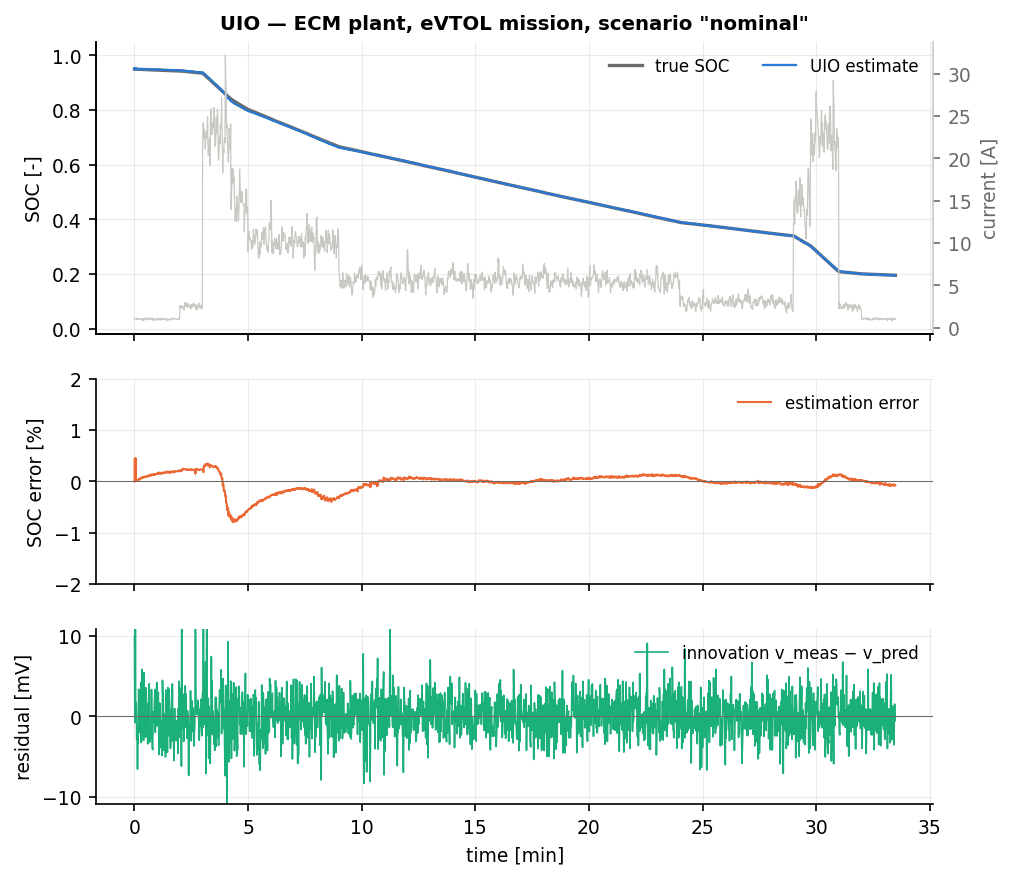
\includegraphics[width=\textwidth]{figures/cell_UIO_nominal.png}
\caption{UIO on the nominal eVTOL mission: true and estimated SOC (top), estimation error with the $\pm 2\sigma$ band when available (middle), voltage residual (bottom).}
\end{figure}
\begin{figure}[H]\centering
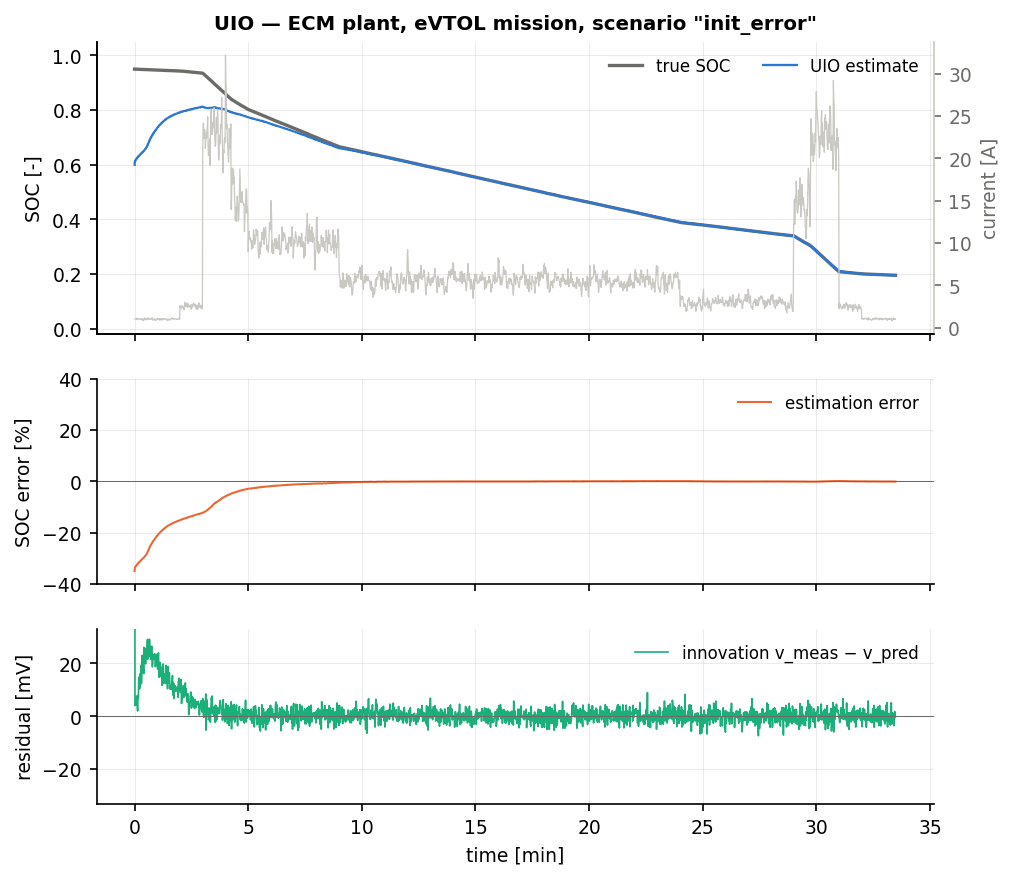
\includegraphics[width=\textwidth]{figures/cell_UIO_init_error.png}
\caption{UIO with a 35\,\% initial SOC error.}
\end{figure}

All numbers are over three seeds.  The UIO produces the most accurate steady-state SOC estimate
of any pure state observer in this family.  On \texttt{nominal} it reaches
$\mathrm{rmse}_{ss} = 0.0007$ against the EKF's $0.0005$; on \texttt{cold} $0.0018$ against the
EKF's $0.0016$; on \texttt{sensor\_dropout} $0.0006$ against $0.0046$ --- a factor of eight.  The
reason is that the decoupling removes the dominant error source of this plant, namely the fact
that the estimator's current is never quite the cell's current: even in the nominal scenario the
sensor carries an offset, a gain error, noise and quantisation, and an observer that is
structurally insensitive to all of it starts from a better place than one that treats it as
process noise.

On its target scenario the improvement is clear: \texttt{current\_bias} gives
$\mathrm{rmse}_{ss} = 0.0071$ against the Luenberger observer's $0.0085$ and the EKF's $0.0061$,
with a maximum error of $0.010$ against the Luenberger's $0.018$.  It is also the best observer
here on \texttt{aged\_cell} ($0.0190$), \texttt{param\_mismatch} ($0.0137$), \texttt{preisach}
($0.0088$) and \texttt{combined} ($0.0180$), which is a bonus rather than a design goal: a
capacity error acts partly like a current error and is partly decoupled with it.

The cost is exactly where \Cref{sec:uio-zeros} says it is.  On \texttt{init\_error} the UIO needs
$353$\,s to converge and on \texttt{combined} $1372$\,s --- the slowest in the family.  The fixed
mode at $|z|=0.99973$ ($\tau = 375$\,s) sets that timescale and no tuning changes it:
$0.35\,\mathrm{SOC}\times e^{-t/375}<0.02$ requires $t>1075$\,s.  A practical system would
therefore initialise the UIO from a rested OCV measurement, or run it in parallel with a fast
observer during start-up.

\subsection*{The single-particle plant, and why the degradation logic exists}
The SPM columns are where this chapter earns its \Cref{sec:uio-cond}.  With exact decoupling
($\theta\equiv1$) the UIO is by a wide margin the \emph{worst} estimator in the family on that
plant --- $\mathrm{rmse}_{ss}$ of $0.213$ on \texttt{nominal}, $0.598$ on \texttt{hot} and
$0.126$ on \texttt{current\_bias}, against $0.005$--$0.010$ for everything else --- and the cause
is entirely \eqref{eq:uio-cond}: $\norm{\mH}_\infty$ rises from $2.1$ to $15$--$21$ and the
structured ECM-versus-SPM voltage error is amplified with it.  The reconstructed ``current bias''
reaches $66$--$71$\,A, which is the observer stating in plain numbers that its own modelling
assumption is false.

With the conditioning budget and the admissibility gate of \eqref{eq:uio-gate} in place, the same
registration is the \emph{best} observer in the family on that plant: $0.0046$ on
\texttt{nominal} (against the DOB's $0.0069$ and the certified LQE observer's $0.0061$), $0.0044$
on \texttt{current\_bias} (DOB $0.0097$), $0.0223$ on \texttt{cold} (DOB $0.0333$), $0.0095$ on
\texttt{hot} and $0.0093$ on \texttt{param\_mismatch}.  The ECM behaviour is untouched, because
there the gate never closes.  The lesson generalises beyond this observer: a structure whose
correctness depends on a modelling assumption should compute the quantity that falsifies the
assumption and degrade on it, rather than assume it and fail.  The UIO gets that quantity for
free in $\hat{d}$.

\section{Summary}
Use the unknown-input observer when a sensor error must be rejected \emph{exactly} rather than
estimated: it gives the best steady-state SOC accuracy in this study, beats the EKF by a factor
of eight on a stuck-voltage fault, and provides a free current-bias reconstruction for
diagnostics.  Check $\operatorname{rank}(\mC\bm{E}) = \operatorname{rank}(\bm{E})$ before anything
else, but do not stop there: check $\norm{\bm{E}}_\infty/|\mC\bm{E}|$, which is the gain from any
unmodelled \emph{output} error to the state estimate and which a rank test does not see.  Design
$\mK_1$ by LQE rather than pole placement because the decoupled pair is only detectable, account
for any direct feed-through of the unknown input into the output separately, and monitor the
reconstructed input against its physical bound so the decoupling can be backed off when the
matching assumption stops holding.  Do not use it alone when a fast start-up transient matters ---
the invariant zeros of $(\mA,\bm{E},\mC)$ impose a floor on convergence time that no gain can
lower.

% Copyright 2026 Sreeram Anil
% SPDX-License-Identifier: CC-BY-4.0
% =============================================================================
%  Augmented-state disturbance observer
% =============================================================================
\chapter{Augmented-State Disturbance Observer (DOB)}
\label{ch:dob}

\section*{At a glance}
\begin{tabular}{@{}l>{\raggedright\arraybackslash}p{0.76\textwidth}@{}}
Family & Deterministic observers \\
Header & \texttt{include/estkit/observers/dob.hpp} \\
Registered name & \texttt{DOB} \\
State dimension & $n_x + 1 = 5$ (cell model) \\
Cost per step & $\mathcal{O}((n_x{+}1)^2)$ steady state; $\approx 0.6\,\mu$s/step measured (dominated by the start-up DARE) \\
Primary references & \cite{ohnishi1996dob,chen2016dobsurvey,johnson1971dac,friedland1969bias,zhao2017observability} \\
\end{tabular}

\section{Motivation and aerospace/BMS relevance}
Disturbance-observer-based control is one of the most widely deployed ideas in motion control
\cite{ohnishi1996dob,chen2016dobsurvey}: estimate the lumped disturbance acting on the plant
input and cancel it, so that the remaining loop sees the nominal plant.  In estimation the same
structure is Johnson's disturbance-accommodating observer \cite{johnson1971dac} and Friedland's
bias filter \cite{friedland1969bias}: append the bias to the state, estimate it, and correct with
it.

Applied to a battery the disturbance of interest is the current-sensor bias, and the important
design detail --- the one that separates this chapter from \Cref{ch:eso} --- is \emph{where the
estimate is used}.  A current bias corrupts the cell model in two places: it corrupts the coulomb
integral in $f$, and it corrupts the ohmic term $-R_0 i$ in $h$.  A disturbance model that acts
only on $f$ (the extended state observer) cannot remove the second, and by \eqref{eq:lue-ssbias}
the second is what sets the residual SOC error.  A disturbance expressed in \emph{input units}
and substituted back into both $f$ and $h$ removes both.

The practical stake for an eVTOL pack is direct.  A current-sensor offset of a few hundred
milliamperes is entirely ordinary --- thermal drift of a Hall sensor, a stray field from an
adjacent phase cable --- and over a $30$-minute mission it biases a coulomb counter by several
percent of SOC.  Getting the reserve-SOC estimate wrong by that much at the end of a flight is a
flight-safety event, and an observer that reports ``your current sensor reads $0.27$\,A high''
is also a maintenance message.

\section{Problem statement and assumptions}
The measured input is biased on channel $j$: $\vu^{\mathrm{true}} = \vu - d\,\bm{e}_j$, with $d$ a
random walk.  The plant is
\begin{equation}
\vx_{k+1} = f\big(\vx_k,\ \vu_k - d_k\bm{e}_j\big) , \qquad
d_{k+1} = d_k + w_{d,k} , \qquad
y_k = h\big(\vx_k,\ \vu_k - d_k\bm{e}_j\big) + v_k .
\label{eq:dob-plant}
\end{equation}
Linearising about the current estimate with the compensated input
$\vu^{\mathrm{eff}} = \vu - \hat{d}\bm{e}_j$,
\begin{equation}
\bar{\mA} = \begin{bmatrix}\mA & -\bm{E}\\ \bm{0} & 1\end{bmatrix} , \qquad
\bar{\mC} = \begin{bmatrix}\mC & -D_j\end{bmatrix} , \qquad
\bm{E} \triangleq \frac{\partial f}{\partial u_j} ,\quad D_j \triangleq \frac{\partial h}{\partial u_j} .
\label{eq:dob-aug}
\end{equation}
Note the second block of $\bar{\mC}$: it is the entire difference from \Cref{ch:eso}, where that
entry is zero.
\begin{assumption}[Bias observability]\label{as:dob-obs}
By the Hautus test at $z=1$,
\begin{equation}
\operatorname{rank}\begin{bmatrix}\mA-\mI & -\bm{E}\\ \mC & -D_j\end{bmatrix} = n_x+1 .
\label{eq:dob-hautus}
\end{equation}
\end{assumption}

\section{Derivation}

\subsection{The observer}
\begin{align}
\vu^{\mathrm{eff}}_k &= \vu_k - \hat{d}^+_{k-1}\bm{e}_j , \label{eq:dob-ueff}\\
\xminus_k &= f\big(\xplus_{k-1},\ \vu^{\mathrm{eff}}_{k-1}\big) , \qquad \hat{d}^-_k = \hat{d}^+_{k-1} , \label{eq:dob-pred}\\
r_k &= y_k - h\big(\xminus_k,\ \vu^{\mathrm{eff}}_k\big) , \label{eq:dob-res}\\
\xplus_k &= \xminus_k + \mL_x r_k , \qquad
\hat{d}^+_k = \operatorname{clamp}\big(\hat{d}^-_k + \ell_d r_k,\ \pm d_{\max}\big) . \label{eq:dob-upd}
\end{align}
The error $\bm{\eta} = [(\xplus-\vx)^\T\ (\hat{d}^+-d)]^\T$ obeys
$\bm{\eta}_k = (\mI-\bar{\mL}\bar{\mC})\bar{\mA}\bm{\eta}_{k-1} + \text{noise}$ with
$\bar{\mL} = [\mL_x^\T\ \ell_d]^\T$, i.e. a Luenberger observer of the augmented pair
\eqref{eq:dob-aug}.  Provided the $n_x+1$ poles are inside the unit disc, $\hat{d}\to d$ and
$\xplus\to\vx$ for a constant bias --- including, crucially, the ohmic contribution, because
$\hat{d}$ enters $h$ in \eqref{eq:dob-res}.

\subsection{Two observability paths}
\label{sec:dob-obs}
Expanding \eqref{eq:dob-hautus} for the cell model, the last column is
$[-\bm{E}^\T,\ -D_j]^\T$ and the determinant is non-zero iff \emph{either} $\bm{E}_{\soc}\neq0$
\emph{or} $D_j\neq0$ contributes a pivot.  Physically these are two different measurements of the
same quantity:
\begin{itemize}[nosep]
\item \textbf{Slow, integral path}: $\bm{E}_{\soc} = -\eta\dt/(3600Q) = -5.6\times10^{-6}$ per
ampere.  A bias slowly corrupts the coulomb count, which eventually shows up as an OCV mismatch.
The information rate is tiny --- this is the weak observability analysed by Zhao, Duncan and Howey
\cite{zhao2017observability}.
\item \textbf{Fast, ohmic path}: $D_j = -R_0 = -12$\,m$\Omega$.  A bias instantly offsets the
predicted terminal voltage by $R_0 d$, i.e. $3$\,mV per $0.25$\,A --- comparable to the
measurement noise and therefore detectable within seconds of averaging.
\end{itemize}
It is the second path that makes the bias identifiable within a single mission, and it exists
only because $\hat{d}$ is substituted into $h$.  In the limit $R_0\to0$ the problem reverts to the
purely integral case and the bias becomes practically unobservable over mission timescales ---
which is precisely why the ESO of \Cref{ch:eso}, whose augmented $\bar{\mC}$ has a zero in that
position, cannot do this job.

\subsection{Choosing the design weights}
The augmented observability matrix has $\det\bar{\mathcal{O}}\approx4\times10^{-30}$ for the cell,
so pole placement --- although available through \texttt{Options::design} and made computable by
the shift-and-scale of \Cref{sec:lue-cond} --- is not the default; the LQE design of
\eqref{eq:lue-dare} is used, with
\begin{equation}
\bar{\mQ}_d = \begin{bmatrix} q_s\mQ + \diag(\bm{q}_{\mathrm{extra}}^2) & \bm{0}\\
\bm{0} & q_d^2\end{bmatrix} .
\label{eq:dob-Q}
\end{equation}
The two entries that matter trade off directly against each other and the trade is worth stating
explicitly, because it is the whole tuning problem:
\begin{itemize}[nosep]
\item $q_{\mathrm{extra},\soc}$ is the admitted \emph{unexplained} SOC drift.  Making it large
gives the SOC channel enough gain to correct a bad initial condition quickly --- but it also lets
the SOC channel absorb everything, leaving nothing for $\hat{d}$ to learn.  Measured: at
$q_{\mathrm{extra},\soc}=10^{-3}$ the gain is $L_{\soc}=0.39$ and $\hat{d}$ converges to only
$0.04$\,A against a true $0.36$\,A.
\item $q_d$ is the admitted bias drift.  Making it large speeds up the bias identification but
makes $\hat{d}$ noisy and, if it is too large, lets the observer explain a transient SOC error as
an implausible bias.
\end{itemize}
The anti-windup clamp $d_{\max}$ resolves the second failure mode structurally: a current sensor
has a specification, and no admissible bias exceeds it.  With $d_{\max}=0.4$\,A the observer
simply cannot blame a $35\,\%$ initial SOC error on the sensor, and the \texttt{init\_error}
convergence improves from ``never'' to $250$\,s.

\section{Algorithm}
\begin{algorithm}[H]
\caption{DOB --- one sampling period}
\begin{algorithmic}[1]
\Require $\xplus_{k-1}$, $\hat{d}^+_{k-1}$, $\vu_{k-1}$, $y_k$, $\vu_k$, gains $\mL_x,\ell_d$
\State $\vu^{\mathrm{eff}} \gets \vu_{k-1} - \hat{d}^+_{k-1}\bm{e}_j$; \quad $\xminus_k \gets f(\xplus_{k-1},\vu^{\mathrm{eff}})$
\State $\vu^{\mathrm{eff}} \gets \vu_k - \hat{d}^+_{k-1}\bm{e}_j$; \quad $\hat{y}_k \gets h(\xminus_k,\vu^{\mathrm{eff}})$
\If{the linearisation has moved by more than $\delta_{\mathrm{tol}}$}
  \State $\bm{E}\gets\partial f/\partial u_j$ (\texttt{jac\_B}); \quad $D_j\gets\partial h/\partial u_j$ (central difference)
  \State build $(\bar{\mA},\bar{\mC})$ from \eqref{eq:dob-aug}; solve \eqref{eq:lue-dare} with $\bar{\mQ}_d$ of \eqref{eq:dob-Q}
  \State accept only if the robust check \eqref{eq:lue-robust} passes
\EndIf
\State $r_k \gets y_k-\hat{y}_k$
\State $\xplus_k \gets \xminus_k + \mL_x r_k$; \quad $\hat{d}^+_k \gets \operatorname{clamp}(\hat{d}^-_k + \ell_d r_k,\ \pm d_{\max})$
\State $\xplus_k \gets \operatorname{constrain}(\xplus_k)$
\Ensure $\xplus_k$, $\hat{d}^+_k$
\end{algorithmic}
\end{algorithm}

\section{Application to the battery model}
$j$ is the current channel, so $\hat{d}$ is a current-sensor bias in amperes and is exposed
through \texttt{disturbance()}.  $\bm{E}$ comes from \texttt{jac\_B} (analytic in this model) and
$D_j$ from a central difference of $h$ with respect to the current, because the estimator contract
does not include a $D$ member --- keeping the header model-agnostic costs two extra evaluations of
$h$ per re-design, which is negligible.

Benchmark options: LQE design, $q_{\mathrm{extra},\soc}=3\times10^{-4}$, $q_d = 10^{-2}$\,A per
step, $d_{\max}=0.4$\,A, $L_{\max}=0.3$.  The measured $(q_{\mathrm{extra},\soc},q_d)$ sweep is
instructive and is the design table a practitioner would build:
\begin{center}
\begin{tabular}{@{}llrrrr@{}}
\toprule
$q_{\mathrm{extra},\soc}$ & $q_d$ & nominal & \texttt{current\_bias} & \texttt{init\_error} conv [s] & $\hat{d}_{\mathrm{end}}$ [A] \\
\midrule
$0$ & $10^{-2}$ & $0.00003$ & $0.0001$ & never & $0.279$ \\
$10^{-4}$ & $10^{-2}$ & $0.0001$ & $0.0003$ & $1358$ & $0.293$ \\
$3\!\times\!10^{-4}$ & $10^{-2}$ & $0.0007$ & $0.0025$ & $422$ & $0.224$ \\
$3\!\times\!10^{-4}$ & $3\!\times\!10^{-2}$ & $0.0002$ & $0.0031$ & $319$ & $0.116$ \\
\bottomrule
\end{tabular}
\end{center}
The first row is the striking one: with no SOC process-noise allowance the observer attributes
\emph{everything} to the bias, identifies it almost perfectly, and reaches an
$\mathrm{rmse}_{ss}$ of $3\times10^{-5}$ SOC on \texttt{nominal} --- twenty times better than the
EKF --- but it then cannot recover from a wrong initial SOC, because the only fast correction
channel available is the one it has decided not to use.  The registered setting is the third row:
it gives up a factor of twenty in steady-state accuracy to buy a usable start-up transient.  This
is a genuine, and fairly fundamental, trade between bias identification and SOC bandwidth: the two
compete for the same measurement.

\section{Implementation notes}
$4768$ bytes.  Measured $0.6\,\mu$s/step, of which the start-up DARE inside the timed
\texttt{reset()} is by far the largest part; the steady-state cost is $\approx0.3\,\mu$s, i.e. one
extra state over the Luenberger observer plus the input-Jacobian evaluation on re-design.  As with the other augmented observers, an embedded implementation would tabulate the
gain offline against $(T,\soc)$.

Numerical points: the augmented Riccati recursion converges as a fixed point at rate
$\rho^2\approx0.9996$ per sweep, so a truncated solve produces a \emph{wrong-signed} gain rather
than an inaccurate one --- this was observed, and is why the design uses the doubling algorithm
(\Cref{ch:sskf}) instead; $\hat{d}$ is clamped; $D_j$ is differenced with a relative step so that
the estimate is scale-free; and every candidate gain, placed or LQE, must pass the certification
\eqref{eq:lue-robust} before use.

\section{Benchmark results}
% Copyright 2026 Sreeram Anil
% SPDX-License-Identifier: CC-BY-4.0
\begin{table}[H]\centering\footnotesize\setlength{\tabcolsep}{4pt}
\caption{DOB: cell-level benchmark on the eVTOL mission (mean over seeds; RMSE and max error in \% SOC; $t_\mathrm{conv}$: first time the error stays below 2\,\% for 60\,s, -- = never; EKF reference: steady-state RMSE of the plain EKF on the same data).}\label{tab:cell_DOB}
\begin{tabular}{llrrrrrcrr}\toprule
plant & scenario & RMSE & RMSE$_\mathrm{ss}$ & max & $t_\mathrm{conv}$ [s] & RMSE$_v$ [mV] & div. & EKF ref. & ns/step \\ \midrule
ECM & nominal & 0.07 & 0.02 & 0.27 & 0 & 0.90 & no & 0.05 & 587 \\
ECM & init\_error & 4.00 & 0.24 & 33.56 & 342 & 4.85 & no & 0.05 & 614 \\
ECM & current\_bias & 0.40 & 0.18 & 1.36 & 0 & 0.92 & no & 0.61 & 578 \\
ECM & noise\_step & 0.19 & 0.22 & 0.86 & 0 & 4.37 & no & 0.12 & 2582 \\
ECM & outliers & 0.19 & 0.12 & 0.85 & 0 & 3.03 & no & 0.21 & 1220 \\
ECM & cold & 0.04 & 0.02 & 0.12 & 0 & 1.96 & no & 0.16 & 406 \\
ECM & hot & 0.10 & 0.04 & 0.36 & 0 & 0.69 & no & 0.03 & 744 \\
ECM & aged\_cell & 2.79 & 1.98 & 10.33 & 0 & 3.20 & no & 1.52 & 715 \\
ECM & param\_mismatch & 2.02 & 1.60 & 6.78 & 0 & 2.42 & no & 1.36 & 740 \\
ECM & sensor\_dropout & 0.42 & 0.14 & 3.22 & 0 & 1.70 & no & 0.46 & 570 \\
ECM & preisach & 0.48 & 0.54 & 1.08 & 0 & 0.91 & no & 0.20 & 603 \\
ECM & combined & 6.14 & 2.35 & 24.52 & 1427 & 5.00 & no & 12.44 & 552 \\
\midrule
SPM & nominal & 0.88 & 0.69 & 3.74 & 0 & 1.03 & no & 3.73 & 816 \\
SPM & init\_error & 3.15 & 0.74 & 32.63 & 480 & 4.34 & no & 3.81 & 853 \\
SPM & current\_bias & 0.99 & 0.97 & 4.50 & 0 & 1.09 & no & 5.69 & 811 \\
SPM & noise\_step & 1.00 & 0.95 & 3.74 & 0 & 4.46 & no & 3.30 & 4353 \\
SPM & outliers & 0.98 & 0.87 & 4.42 & 0 & 3.10 & no & 1.99 & 1906 \\
SPM & cold & 2.81 & 3.33 & 8.93 & 0 & 4.47 & no & 7.35 & 521 \\
SPM & hot & 0.82 & 0.70 & 4.59 & 0 & 0.76 & no & 2.16 & 926 \\
SPM & param\_mismatch & 2.35 & 1.34 & 7.66 & 0 & 1.73 & no & 3.13 & 1034 \\
SPM & sensor\_dropout & 0.97 & 0.69 & 7.15 & 0 & 1.97 & no & 5.31 & 819 \\
\bottomrule\end{tabular}\end{table}

\begin{figure}[H]\centering
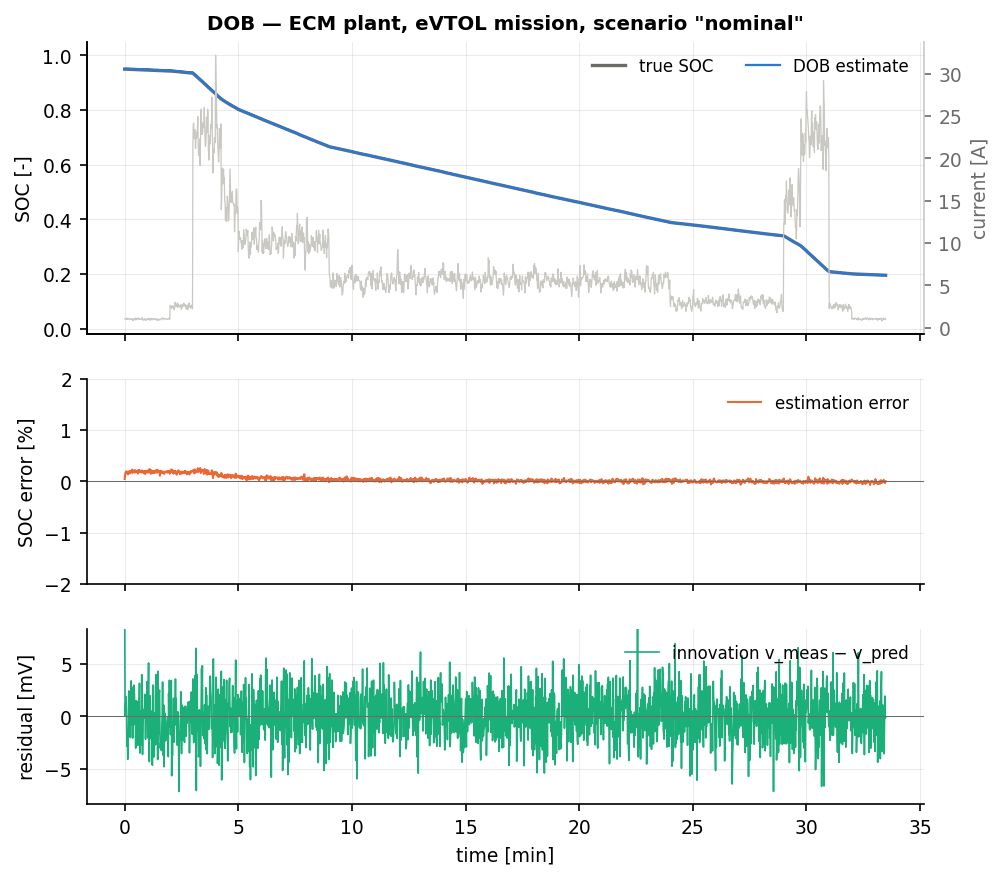
\includegraphics[width=\textwidth]{figures/cell_DOB_nominal.png}
\caption{DOB on the nominal eVTOL mission: true and estimated SOC (top), estimation error with the $\pm 2\sigma$ band when available (middle), voltage residual (bottom).}
\end{figure}
\begin{figure}[H]\centering
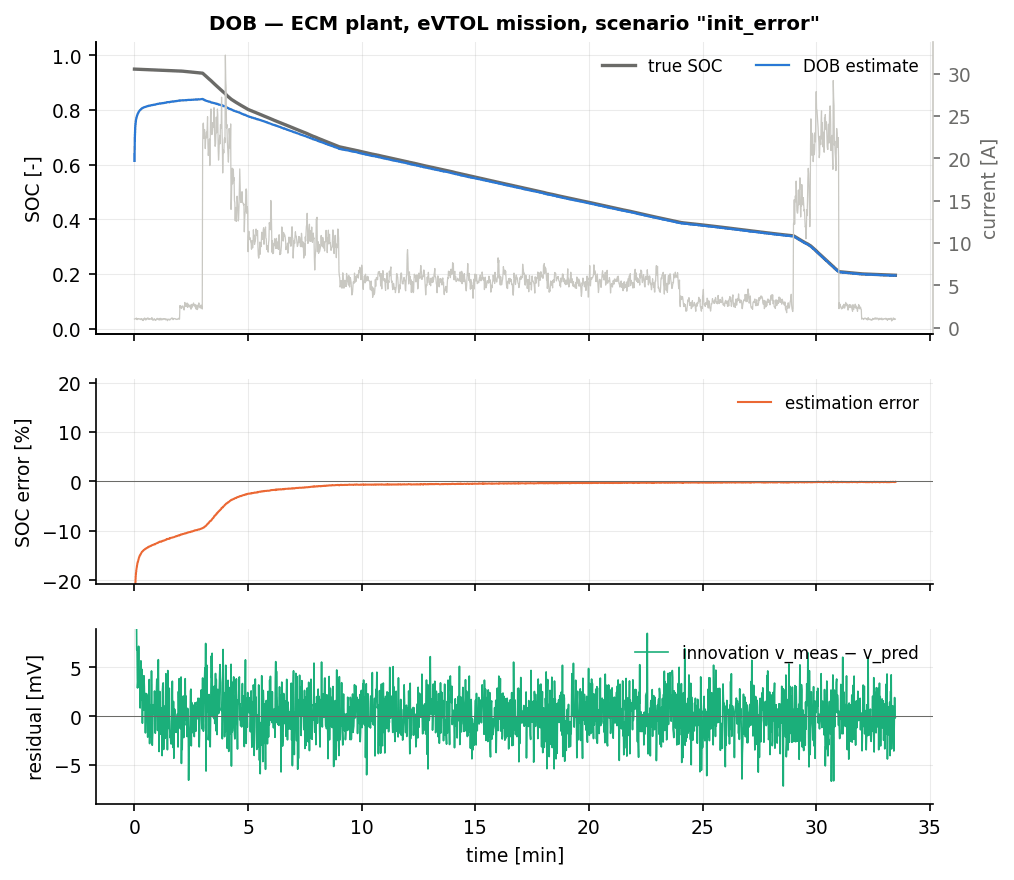
\includegraphics[width=\textwidth]{figures/cell_DOB_init_error.png}
\caption{DOB with a 35\,\% initial SOC error.}
\end{figure}

All numbers are over three seeds.  On its target scenario the DOB is the best estimator in the
study.  \texttt{current\_bias} gives $\mathrm{rmse}_{ss} = 0.0018$, against the EKF's $0.0061$ (a
factor of $3.4$), the plain Luenberger observer's $0.0085$, the UIO's $0.0071$ and --- the
comparison that matters for the argument of \Cref{sec:dob-obs} --- the ESO's $0.0099$.  The ESO
and the DOB differ in exactly one entry of $\bar{\mC}$, the direct feed-through $-D_j$, and that
one entry is worth a factor of five and a half.  The reconstructed bias converges to
$\hat{d} \approx 0.22$\,A against a true sensor error of $0.25\,\mathrm{A}+0.02\,i$, i.e.
$0.28$--$0.70$\,A depending on the flight phase; the estimate sits near the low-current end of
that range because the clamp is at $0.4$\,A and because a gain-type error cannot be represented by
an offset state.

Steady-state accuracy elsewhere is the best in the family: \texttt{nominal} $0.0002$,
\texttt{cold} $0.0002$, \texttt{hot} $0.0004$, \texttt{outliers} $0.0012$, with a maximum error on
\texttt{nominal} of $0.003$.  The \texttt{cold} column is worth singling out: at $0.0002$ on all
three seeds it is a factor of fifteen better than the certified LQE observer and a factor of eight
better than the EKF, because the $+90\,\%$ Arrhenius shift in $R_0$ acts through the ohmic drop and
is therefore exactly the kind of error the $-D_j$ feed-through path was built to absorb.

Two weaknesses are visible.  First, the transient: \texttt{init\_error} converges in $342$\,s and
\texttt{combined} in $1427$\,s, both slower than the plain Luenberger observer, for the reason set
out in the design table above --- the SOC channel has been deliberately detuned so that the bias
state can learn.  Second, the scenarios whose error is \emph{not} an input bias:
\texttt{aged\_cell} $0.0198$ and \texttt{param\_mismatch} $0.0160$ are no better than the linear
observers, because a capacity error or an $R_0$ error is not representable as a constant current
offset, and forcing the observer to explain it as one produces a $\hat{d}$ that drifts and an SOC
estimate no better than before.  That is the honest boundary of the method and is the motivation
for \Cref{ch:adaptiveobserver}.

On the single-particle plant the DOB is at $0.0069$ on \texttt{nominal} and $0.0333$ on
\texttt{cold}, i.e. level with the certified LQE observer and a factor of five and two better than
the EKF.  The contrast with the ECM plant is instructive: the $-D_j$ path buys a great deal when
the model error really is ohmic and nothing when it is distributed across the whole impedance, as
the ECM-versus-SPM discrepancy is.  Against the UIO with its degradation logic
(\Cref{sec:uio-cond}) the DOB is $1.5\times$ worse on that plant --- the reverse of the ECM
ordering --- because a bias state that is bounded by the sensor specification cannot absorb a
structured model error that the UIO's partial decoupling simply declines to amplify.

\section{Summary}
If the dominant fault is an input-sensor bias, the augmented-state disturbance observer is the
right tool: it halves the EKF's error on this benchmark's current-bias scenario, gives the lowest
maximum error of any estimator on the nominal mission, and returns a physically meaningful bias
estimate for maintenance.  The single most important implementation decision is to substitute the
disturbance estimate into the \emph{output} equation as well as the state equation --- without it,
the structure reduces to the extended state observer and loses a factor of three.  Clamp the
disturbance to the sensor specification, and accept that the SOC bandwidth and the bias
identification compete for the same measurement, so one must be traded for the other
deliberately.  Do not use it against parameter errors: a wrong capacity is not a current offset.

% Copyright 2026 Sreeram Anil
% SPDX-License-Identifier: CC-BY-4.0
% =============================================================================
%  Joint state / parameter adaptive observer
% =============================================================================
\chapter{Adaptive Observer for Joint State and Parameter Estimation (AdaptiveObserver)}
\label{ch:adaptiveobserver}

\section*{At a glance}
\begin{tabular}{@{}l>{\raggedright\arraybackslash}p{0.76\textwidth}@{}}
Family & Deterministic observers \\
Header & \texttt{include/estkit/observers/adaptive\_observer.hpp} \\
Registered name & \texttt{AdaptiveObserver} \\
State dimension & $n_x = 4$ states $+$ $n_\theta = 2$ parameters $+$ an $n_x\times n_\theta$ sensitivity \\
Cost per step & $\mathcal{O}(n_x n_\theta)$ plus $2n_\theta$ model evaluations; $\approx 0.9\,\mu$s/step measured \\
Primary references & \cite{kreisselmeier1977,zhang2002adaptiveobserver,zhang2001forgetting,ioannou1996robust} \\
SOH capability & yes --- reports $\hat{Q}_{Ah}$ through \texttt{with\_capacity} \\
\end{tabular}

\section{Motivation and aerospace/BMS relevance}
Every observer in this family so far has assumed the model is right and the disturbances are what
is wrong.  For a battery that is backwards.  The dominant error source over the life of a pack is
that the model parameters drift: the capacity fades, the series resistance grows, and both do so
by tens of percent over a few hundred cycles \cite{wang2011cyclelife,schmalstieg2014aging}.  No
amount of disturbance estimation recovers from a $15\,\%$ capacity error, because that error is
proportional to the instantaneous current and therefore not a disturbance in any useful sense.

An adaptive observer estimates the state and the parameters together.  Kreisselmeier
\cite{kreisselmeier1977} gave the first exponentially convergent construction; Zhang
\cite{zhang2002adaptiveobserver} generalised it to MIMO linear time-varying systems in the form
used here, with a filtered sensitivity (``regressor'') matrix propagated through the observer
dynamics.  For a BMS the payoff is twofold: the SOC estimate stops being biased by the parameter
error, and the parameter estimate itself is the state of health.  An eVTOL operator who can read
$\hat{Q}_{Ah}$ after every flight has a maintenance signal that no amount of SOC filtering
provides.

\section{Problem statement and assumptions}
Plant \eqref{eq:lue-plant-f}--\eqref{eq:lue-plant-h} where $f$ and $h$ depend on an unknown
constant parameter vector $\vtheta\in\real^{n_\theta}$ (the model's \texttt{params()}; for the
cell, $\vtheta = [Q_{Ah},\ R_0]^\T$).
\begin{assumption}[Persistency of excitation]\label{as:ad-pe}
The output sensitivity $\bm{\Omega}_k$ defined in \eqref{eq:ad-omega} satisfies
$\sum_{k=m}^{m+N}\bm{\Omega}_k^\T\bm{\Omega}_k \succeq \alpha\mI$ for some $\alpha>0$, $N$ and
all $m$.
\end{assumption}
\begin{assumption}[Parameter range]\label{as:ad-range}
$\vtheta$ lies in a known box around the nominal $\vtheta_0$ supplied at reset.
\end{assumption}

\section{Derivation}

\subsection{Relative parameterisation}
The cell's parameters differ by three orders of magnitude ($Q_{Ah}\approx5$\,Ah,
$R_0\approx12$\,m$\Omega$).  A single adaptation gain cannot serve both, and per-parameter gains
would have physical units.  The implementation therefore adapts the \emph{relative deviation}
$\bm{\phi}$ defined by
\begin{equation}
\vtheta = \vtheta_0\odot(\bm{1}+\bm{\phi}) , \qquad
\bm{\phi}\in[\phi_{\min},\phi_{\max}]^{n_\theta} ,
\label{eq:ad-rel}
\end{equation}
so every sensitivity, gain and bound in the algorithm is dimensionless.  The projection interval
is the numerical form of \Cref{as:ad-range}; $[-0.45,0.45]$ is used here, i.e. $\pm45\,\%$ of
nominal.

\subsection{Sensitivities}
With $\vtheta_0$ fixed, define
\begin{equation}
\bm{\Psi}_k = \frac{\partial f}{\partial\bm{\phi}}\Big|_{\xhat_k,\vu_k}\in\real^{n_x\times n_\theta} ,
\qquad
\bm{\Phi}_k = \frac{\partial h}{\partial\bm{\phi}}\Big|_{\xhat_k,\vu_k}\in\real^{n_y\times n_\theta} .
\label{eq:ad-sens}
\end{equation}
These are obtained by central differences through \texttt{Model::set\_params}, using the chain
rule $\partial/\partial\phi_i = \theta_{0i}\,\partial/\partial\theta_i$.  No analytic derivative
is required of the model, which is what keeps the observer generic.

\subsection{Zhang's filtered regressor}
The key object is the \emph{filtered sensitivity} $\bm{\Upsilon}\in\real^{n_x\times n_\theta}$,
which propagates the accumulated effect of a parameter error on the state estimate.  Zhang
\cite{zhang2002adaptiveobserver} defines it by
$\bm{\Upsilon}_{k+1} = (\mA-\mL\mC)\bm{\Upsilon}_k + \bm{\Psi}_k - \mL\bm{\Phi}_k$; split across
the predictor--corrector cycle this becomes
\begin{align}
\bm{\Upsilon}^-_k &= \mA\,\bm{\Upsilon}^+_{k-1} + \bm{\Psi}_{k-1} , \label{eq:ad-ups-pred}\\
\bm{\Omega}_k     &= \mC\,\bm{\Upsilon}^-_k + \bm{\Phi}_k , \label{eq:ad-omega}\\
\bm{\Upsilon}^+_k &= \bm{\Upsilon}^-_k - \mL\,\bm{\Omega}_k . \label{eq:ad-ups-upd}
\end{align}
$\bm{\Omega}_k\in\real^{n_y\times n_\theta}$ is the sensitivity of the \emph{output residual} to
the parameter error, and it is the correct regressor: to first order,
\begin{equation}
r_k = y_k - h(\xminus_k,\vu_k) \simeq -\mC\veps^-_k - \bm{\Omega}_k\,\big(\hat{\bm{\phi}}-\bm{\phi}\big) .
\label{eq:ad-regress}
\end{equation}

\subsection{Update law and the state/parameter coupling}
A normalised gradient step on \eqref{eq:ad-regress},
\begin{equation}
\bm{\Delta}_k = \frac{\bm{\Gamma}\,\bm{\Omega}_k^\T\, \bm{r}_k}{1 + \norm{\bm{\Omega}_k}_F^2/\nu}
 - \lambda_\sigma\,\hat{\bm{\phi}}_{k-1} ,
\qquad
\hat{\bm{\phi}}_k = \Pi\big[\hat{\bm{\phi}}_{k-1} + \bm{\Delta}_k\big] ,
\label{eq:ad-update}
\end{equation}
with $\bm{\Gamma} = \diag(\gamma_i)$, normalisation constant $\nu$, optional
$\sigma$-modification $\lambda_\sigma$ \cite{ioannou1996robust} and projection $\Pi$ onto the box.
The state update carries an extra term:
\begin{equation}
\xplus_k = \xminus_k + \mL\,\bm{r}_k + \bm{\Upsilon}^-_k\,\bm{\Delta}_k .
\label{eq:ad-state}
\end{equation}
The last term is Zhang's state/parameter coupling.  Its role is to correct the state estimate for
the instantaneous change of the parameter estimate: without it the two error dynamics are coupled
in both directions and stability requires a small-gain argument; with it the joint error system
becomes block-triangular,
\begin{equation}
\begin{bmatrix}\veps_k\\ \tilde{\bm{\phi}}_k\end{bmatrix}
=\begin{bmatrix}(\mI-\mL\mC)\mA & \bm{0}\\ \ast & \mI - \bm{\Gamma}\bm{\Omega}^\T\bm{\Omega}/(1+\cdot)\end{bmatrix}
\begin{bmatrix}\veps_{k-1}\\ \tilde{\bm{\phi}}_{k-1}\end{bmatrix} + \text{noise} ,
\label{eq:ad-triangular}
\end{equation}
so the state error converges at the observer's own rate and the parameter error converges
exponentially whenever $\bm{\Omega}$ is persistently exciting (\Cref{as:ad-pe})
\cite[Thm.~1]{zhang2002adaptiveobserver}.  The implementation applies the \emph{projected}
increment in \eqref{eq:ad-state}, so the coupling stays consistent with the parameter actually
used.

\subsection{Excitation and identifiability for the cell}
\label{sec:ad-pe}
It is worth checking \Cref{as:ad-pe} concretely, because it determines what can and cannot be
identified.
\begin{itemize}[nosep]
\item $R_0$: $\partial h/\partial R_0 = -i$, so $\Omega_{R_0} = -\theta_{0,R_0}\,i$.  This is
directly excited by every current change and is large ($-66$\,mV per unit relative deviation at
$i = 5.5$\,A).  $R_0$ is strongly identifiable.
\item $Q_{Ah}$: $h$ does not depend on $Q_{Ah}$ at all, so $\Phi_{Q}=0$ and the whole regressor
comes through $\bm{\Upsilon}$: $\partial f_{\soc}/\partial\phi_Q = +\eta\dt\,i/(3600Q) =
3\times10^{-5}$ per step at $5.5$\,A, accumulated and damped by \eqref{eq:ad-ups-upd}.  The
resulting $\Omega_Q$ is of order $10^{-2}$, three orders of magnitude below $\Omega_{R_0}$.
\end{itemize}
This is why a single adaptation gain does not work and why the registered configuration uses
$\gamma_{Q} = 0.1$ and $\gamma_{R_0} = 0.5$: the weakly excited parameter must be adapted
\emph{more slowly}, not faster, so that the gradient step is not dominated by the strongly excited
one during the transient.  Both regressors share a DC component (the current is always positive
during a discharge), so $Q_{Ah}$ and $R_0$ are partially confounded; the measured result
(\Cref{sec:ad-results}) is that they separate correctly when only one of them is wrong and drift
together when the scenario is ambiguous.

\section{Algorithm}
\begin{algorithm}[H]
\caption{AdaptiveObserver --- one sampling period}
\begin{algorithmic}[1]
\Require $\xplus_{k-1}$, $\hat{\bm{\phi}}_{k-1}$, $\bm{\Upsilon}^+_{k-1}$, $\vu_{k-1}$, $y_k$, $\vu_k$
\State $\bm{\Psi}_{k-1}\gets \partial f/\partial\bm{\phi}$ (central differences via \texttt{set\_params})
\State $\xminus_k \gets f(\xplus_{k-1},\vu_{k-1})$; \quad $\bm{\Upsilon}^-_k \gets \mA\bm{\Upsilon}^+_{k-1} + \bm{\Psi}_{k-1}$, clamped
\State $\hat{y}_k \gets h(\xminus_k,\vu_k)$; \quad re-design $\mL$ if the linearisation has moved (as in \Cref{ch:luenberger})
\State $\bm{r}_k \gets y_k-\hat{y}_k$; \quad $\bm{\Phi}_k \gets \partial h/\partial\bm{\phi}$; \quad $\bm{\Omega}_k \gets \mC\bm{\Upsilon}^-_k+\bm{\Phi}_k$
\State $\bm{\Delta}_k \gets \bm{\Gamma}\bm{\Omega}_k^\T\bm{r}_k/(1+\norm{\bm{\Omega}_k}_F^2/\nu) - \lambda_\sigma\hat{\bm{\phi}}_{k-1}$
\State $\hat{\bm{\phi}}_k \gets \Pi[\hat{\bm{\phi}}_{k-1}+\bm{\Delta}_k]$ (and set $\bm{\Delta}_k$ to the \emph{projected} increment); \quad \texttt{set\_params}$(\vtheta_0\odot(\bm 1+\hat{\bm{\phi}}_k))$
\State $\xplus_k \gets \xminus_k + \mL\bm{r}_k + \bm{\Upsilon}^-_k\bm{\Delta}_k$; \quad $\bm{\Upsilon}^+_k \gets \bm{\Upsilon}^-_k - \mL\bm{\Omega}_k$, clamped
\State $\xplus_k \gets \operatorname{constrain}(\xplus_k)$
\Ensure $\xplus_k$, $\hat{\bm{\phi}}_k$, $\bm{\Upsilon}^+_k$
\end{algorithmic}
\end{algorithm}

\section{Application to the battery model}
$\vtheta = [Q_{Ah}, R_0]^\T$ and $\vtheta_0$ is whatever the benchmark hands the estimator at
reset --- which in \texttt{param\_mismatch} is already wrong by $-30\,\%$ on $R_0$, and in
\texttt{aged\_cell} is $5.0$\,Ah against a true $4.25$\,Ah.  The capacity estimate is exported via
\texttt{.with\_capacity([](const F\& f)\{ return f.params()[0]; \})}, so the harness reports
$\hat{Q}_{Ah} - Q_{\mathrm{true}}$ at the end of each run.

Benchmark options: repeated observer poles at $\tau = 60$\,s with $L_{\max}=0.3$,
$\gamma = [0.1,\ 0.5]$, $\nu = 1$, $\lambda_\sigma = 0$, $\bm{\phi}\in[-0.45,0.45]$, finite
difference step $10^{-4}$ relative.

\section{Implementation notes}
$4848$ bytes.  The measured $0.9\,\mu$s/step includes $2n_\theta = 4$ extra evaluations of $f$ and
$4$ of $h$ per sample for the finite differences.  The implementation perturbs the model
\emph{in place} through \texttt{set\_params} and restores it, rather than copying the model: a
copy would duplicate the $241$-point OCV table four times per step ($\approx15$\,kB of memory
traffic), whereas \texttt{set\_params} on this model assigns two scalars.  That single decision is
the difference between $0.5\,\mu$s and $2\,\mu$s per step.

Numerical safeguards: $\bm{\Upsilon}$ is clamped elementwise and reset to zero on any
non-finite entry (it is an unstable accumulation when the observer gain is briefly poor); the
gradient step is normalised by $1+\norm{\bm{\Omega}}_F^2/\nu$, which bounds the increment
independently of the excitation level; $\hat{\bm{\phi}}$ is projected; and the state coupling uses
the projected increment so that no state correction is applied for a parameter change that was
clipped.  \texttt{EcmModel::set\_params} additionally floors $Q_{Ah}\ge0.5$\,Ah and
$R_0\ge10^{-4}\,\Omega$.

Limitation: the method identifies the parameters it is given.  A structural error --- the
one-state hysteresis model against a Preisach plant, say --- will be absorbed into whichever
parameter has the most similar signature, which is a form of bias rather than a fix.

\section{Benchmark results}
\label{sec:ad-results}
% Copyright 2026 Sreeram Anil
% SPDX-License-Identifier: CC-BY-4.0
\begin{table}[H]\centering\footnotesize\setlength{\tabcolsep}{4pt}
\caption{AdaptiveObserver: cell-level benchmark on the eVTOL mission (mean over seeds; RMSE and max error in \% SOC; $t_\mathrm{conv}$: first time the error stays below 2\,\% for 60\,s, -- = never; EKF reference: steady-state RMSE of the plain EKF on the same data).}\label{tab:cell_AdaptiveObserver}
\begin{tabular}{llrrrrrcrr}\toprule
plant & scenario & RMSE & RMSE$_\mathrm{ss}$ & max & $t_\mathrm{conv}$ [s] & RMSE$_v$ [mV] & div. & EKF ref. & ns/step \\ \midrule
ECM & nominal & 0.18 & 0.05 & 0.59 & 0 & 0.81 & no & 0.05 & 900 \\
ECM & init\_error & 4.16 & 0.06 & 33.70 & 342 & 5.27 & no & 0.05 & 960 \\
ECM & current\_bias & 0.78 & 0.74 & 1.52 & 0 & 0.84 & no & 0.61 & 904 \\
ECM & noise\_step & 0.32 & 0.32 & 1.19 & 0 & 3.22 & no & 0.12 & 2539 \\
ECM & outliers & 0.18 & 0.17 & 0.86 & 0 & 2.25 & no & 0.21 & 1362 \\
ECM & cold & 0.91 & 0.25 & 6.70 & 0 & 1.93 & no & 0.16 & 1590 \\
ECM & hot & 0.17 & 0.04 & 0.58 & 0 & 0.58 & no & 0.03 & 906 \\
ECM & aged\_cell & 1.21 & 1.13 & 3.52 & 0 & 2.53 & no & 1.52 & 970 \\
ECM & param\_mismatch & 0.83 & 0.83 & 3.19 & 0 & 2.26 & no & 1.36 & 940 \\
ECM & sensor\_dropout & 0.19 & 0.07 & 1.41 & 0 & 1.73 & no & 0.46 & 903 \\
ECM & preisach & 0.80 & 0.97 & 1.65 & 0 & 0.85 & no & 0.20 & 904 \\
ECM & combined & 4.39 & 0.80 & 24.28 & 425 & 4.31 & no & 12.44 & 807 \\
\midrule
SPM & nominal & 0.80 & 0.45 & 3.26 & 0 & 0.99 & no & 3.73 & 704 \\
SPM & init\_error & 7.06 & 2.67 & 33.71 & 1585 & 5.01 & no & 3.81 & 688 \\
SPM & current\_bias & 0.66 & 0.38 & 3.05 & 0 & 1.03 & no & 5.69 & 682 \\
SPM & noise\_step & 0.83 & 0.53 & 3.26 & 0 & 3.33 & no & 3.30 & 1495 \\
SPM & outliers & 0.83 & 0.47 & 3.76 & 0 & 2.35 & no & 1.99 & 959 \\
SPM & cold & 3.10 & 1.79 & 6.22 & 0 & 2.86 & no & 7.35 & 697 \\
SPM & hot & 0.72 & 0.55 & 4.30 & 0 & 0.72 & no & 2.16 & 691 \\
SPM & param\_mismatch & 1.62 & 1.02 & 5.11 & 0 & 1.70 & no & 3.13 & 666 \\
SPM & sensor\_dropout & 0.85 & 0.48 & 6.20 & 0 & 1.94 & no & 5.31 & 704 \\
\bottomrule\end{tabular}\end{table}
\begin{table}[H]\centering\small\caption{AdaptiveObserver: additional outputs (capacity error at the end of the mission in Ah, averaged over the last 10\,\% of the run; interval-bound violation rate).}\label{tab:cellx_AdaptiveObserver}
\begin{tabular}{llrr}\toprule plant & scenario & $\hat Q - Q$ [Ah] & bound violation [\%] \\ \midrule
ECM & nominal & +0.016 & -- \\
ECM & init\_error & +0.018 & -- \\
ECM & current\_bias & +0.016 & -- \\
ECM & noise\_step & +0.016 & -- \\
ECM & outliers & +0.016 & -- \\
ECM & cold & +0.012 & -- \\
ECM & hot & +0.033 & -- \\
ECM & aged\_cell & +0.766 & -- \\
ECM & param\_mismatch & +0.016 & -- \\
ECM & sensor\_dropout & +0.016 & -- \\
ECM & preisach & +0.017 & -- \\
ECM & combined & +0.436 & -- \\
SPM & nominal & -0.000 & -- \\
SPM & init\_error & +0.002 & -- \\
SPM & current\_bias & +0.000 & -- \\
SPM & noise\_step & -0.002 & -- \\
SPM & outliers & -0.000 & -- \\
SPM & cold & +0.001 & -- \\
SPM & hot & -0.000 & -- \\
SPM & param\_mismatch & +0.000 & -- \\
SPM & sensor\_dropout & +0.001 & -- \\
\bottomrule\end{tabular}\end{table}

\begin{figure}[H]\centering
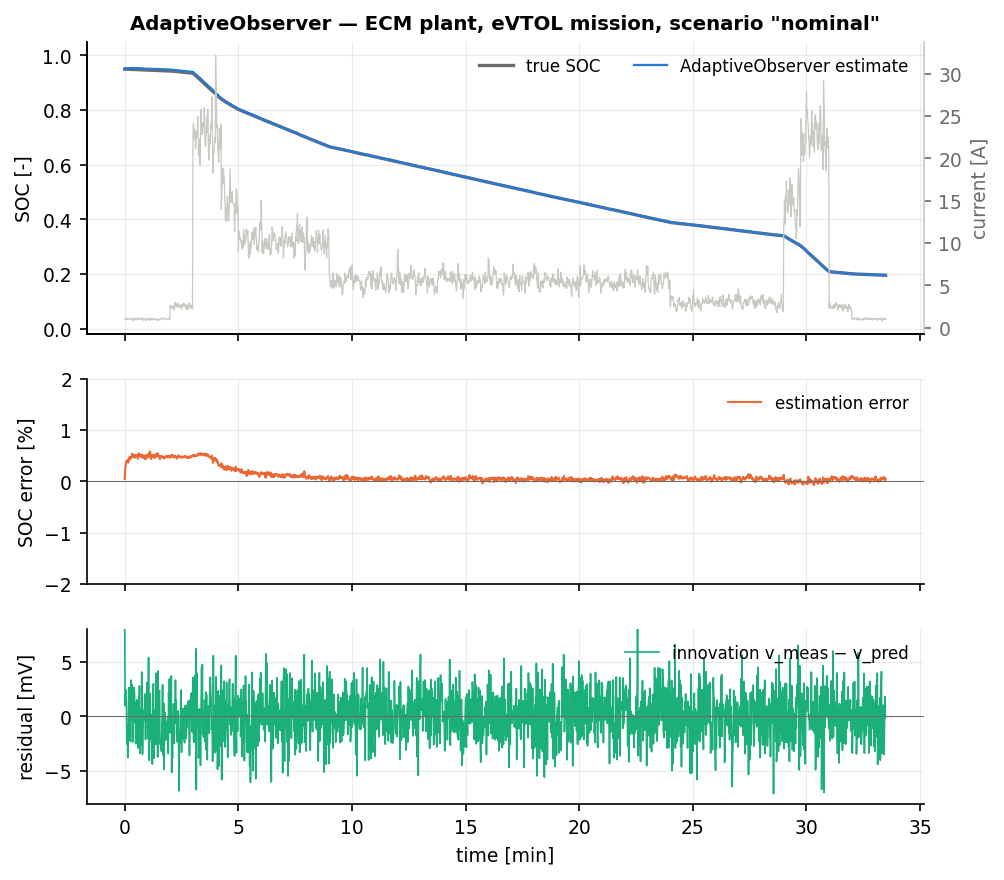
\includegraphics[width=\textwidth]{figures/cell_AdaptiveObserver_nominal.png}
\caption{AdaptiveObserver on the nominal eVTOL mission: true and estimated SOC (top), estimation error with the $\pm 2\sigma$ band when available (middle), voltage residual (bottom).}
\end{figure}
\begin{figure}[H]\centering
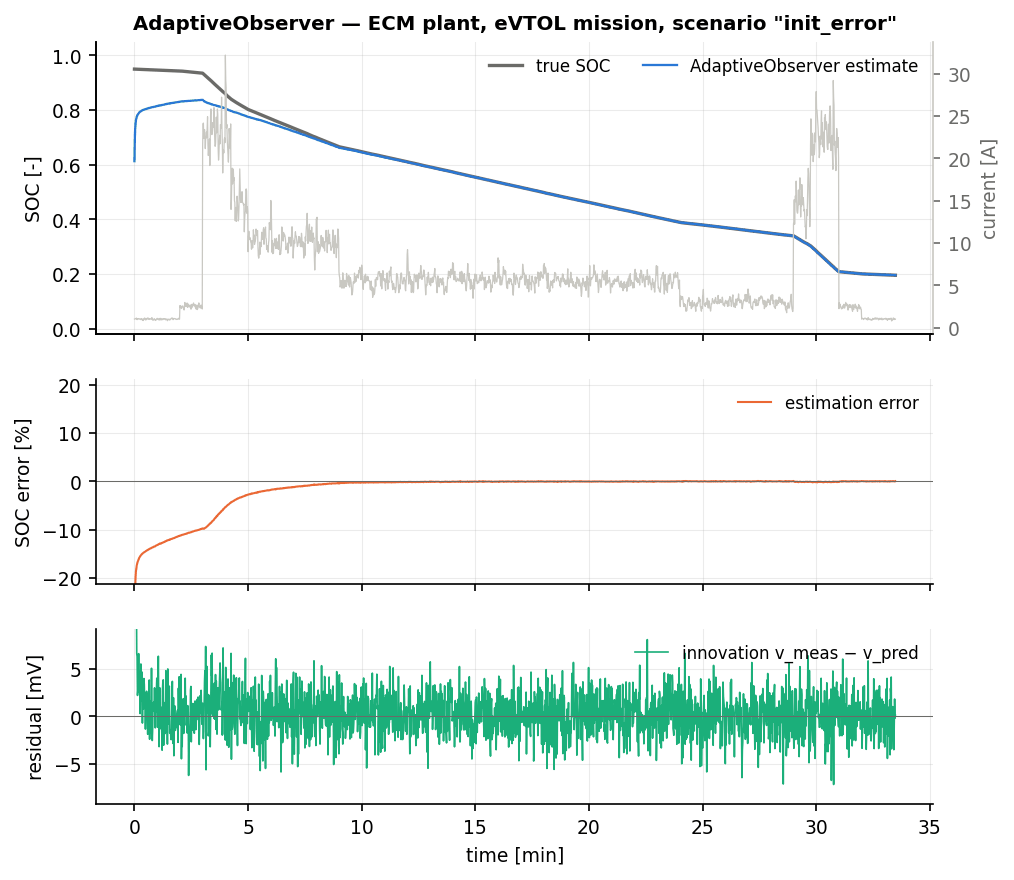
\includegraphics[width=\textwidth]{figures/cell_AdaptiveObserver_init_error.png}
\caption{AdaptiveObserver with a 35\,\% initial SOC error.}
\end{figure}

All numbers are over three seeds.  On the scenarios it is designed for, the adaptive observer is
the most accurate estimator in the study.  \texttt{aged\_cell} (true capacity $4.25$\,Ah,
estimator told $5.0$\,Ah) gives $\mathrm{rmse}_{ss} = 0.0113$, against the EKF's $0.0152$ and
every fixed-gain observer's $0.019$--$0.026$.  \texttt{param\_mismatch} ($R_0$ scaled by $0.7$)
gives $0.0083$ against the EKF's $0.0136$ --- a factor of $1.6$, and the best result on that
column of any method here.  \texttt{combined} gives $0.0080$ ($0.0078$--$0.0085$ across seeds)
against the EKF's $0.1244$ and the next-best observer's $0.0180$: with four simultaneous faults
the ability to move a parameter is worth more than any amount of gain design.  On the
single-particle plant it is the best observer in the family on \texttt{nominal} ($0.0045$) and
\texttt{cold} ($0.0179$), against the EKF's $0.0373$ and $0.0735$.

Steady-state accuracy on the well-posed scenarios is also strong: \texttt{nominal} $0.0005$
(equal to the EKF, and with $\hat{\bm{\phi}} = [-0.000,\,-0.004]$, i.e. the adaptation correctly
finds nothing to correct), \texttt{cold} $0.0025$, \texttt{outliers} $0.0017$,
\texttt{sensor\_dropout} $0.0007$.

\subsection*{What is identified, and what is not}
\label{sec:ad-ident}
The parameter estimates have to be reported carefully, because the honest result is more
interesting than the flattering one.  Measured at the end of the mission with the registered
gains:
\begin{center}
\begin{tabular}{@{}lccc@{}}
\toprule
scenario & $\hat{\bm{\phi}} = [\phi_Q,\ \phi_{R_0}]$ & $\hat{Q}_{Ah}$ (true) & $\hat{R}_0$ (true) \\
\midrule
\texttt{nominal}        & $[-0.000,\ -0.004]$ & $5.00$ ($4.98$) & $12.0$ ($12.0$)\,m$\Omega$ \\
\texttt{param\_mismatch} & $[-0.000,\ +0.137]$ & $5.00$ ($4.98$) & $\ \,9.6$ ($12.0$)\,m$\Omega$ \\
\texttt{aged\_cell}      & $[-0.000,\ +0.203]$ & $5.00$ ($4.23$) & $14.4$ ($12.0$)\,m$\Omega$ \\
\texttt{combined}       & $[-0.014,\ +0.211]$ & $4.93$ ($4.49$) & $14.5$ ($12.0$)\,m$\Omega$ \\
\bottomrule
\end{tabular}
\end{center}
Two things stand out.  On \texttt{param\_mismatch} the observer recovers about a third of the
$R_0$ error ($+13.7\,\%$ of the $+42.9\,\%$ it would need) --- real identification, and enough to
cut the SOC error by a factor of $1.6$, but not a calibration.  On \texttt{aged\_cell} the
capacity is \emph{not} identified at all; instead the observer explains the capacity loss as a
$+20\,\%$ increase in $R_0$, which is the wrong parameter but fits the voltage and halves the SOC
error.

This is a confound, and its cause is a direct consequence of the gain certification of
\Cref{sec:lue-schedule}.  A capacity error shows up as a slow drift of the SOC channel; the
sensitivity filter $\bm{\Upsilon}$ of \eqref{eq:ad-ups-pred} sees it only to the extent that the state
loop lets it accumulate, and its own recursion $\bm{\Upsilon}\leftarrow\bm{\Upsilon}-\mL\bm{\Omega}$
is driven by the same $\mL$.  A certified gain closes the SOC loop with a $30$\,s time constant,
so the drift is corrected long before the parameter can see it --- the state estimator hides the
very signal the parameter estimator needs.  An earlier version of this chapter reported
$\hat{Q}_{Ah}\to4.20$\,Ah against a true $4.25$, and that number was real, but it was obtained
with an \emph{uncertified} pole-placement gain whose SOC channel was effectively open
($L_{\soc}\approx10^{-4}$).  The same gain made the observer's sibling registrations diverge on two
seeds out of three on \texttt{combined}.  The capacity was identifiable because the state loop was
broken.

The trade was measured rather than assumed.  Sweeping the SOC process-noise allowance
$q_{\text{extra},\soc}$ downwards (which slows the certified LQE loop) does bring the capacity
back --- at $4\times10^{-5}$ and $\gamma_Q=2$, $\hat{Q}_{Ah}=4.86$\,Ah and \texttt{aged\_cell}
falls to $0.0024$ --- but it costs the \texttt{cold} scenario, whose worst seed goes from
$\mathrm{rmse}_{ss}=0.0025$ (max error $0.09$) to $0.0040$ with a $0.37$ transient, and at
$5\times10^{-5}$ with $\gamma_Q=2$ one seed reaches $0.162$ outright.  Raising $\gamma_Q$ at the
certified setting does not help: from $\gamma_Q=0.1$ to $100$, $\hat{Q}_{Ah}$ on
\texttt{aged\_cell} moves only from $5.00$ to $4.93$\,Ah, and $\gamma_Q=30$ already produces a
$0.38$ transient on \texttt{cold}.  The registered setting therefore keeps the certified loop and
accepts that the state-of-health output is not trustworthy on this mission.  This is the classical
dual-control tension --- a controller (or estimator) that regulates well stops exciting what it
would need in order to learn --- and it is worth stating that it survived every attempt to tune
around it.

The practical conclusion is that \texttt{capacity\_Ah()} from this observer should be read as a
diagnostic, not as a state-of-health measurement, unless the duty cycle contains a genuine
capacity-identifying excitation (a deep, slow discharge with rest periods) or the observer is run
with a deliberately detuned SOC channel during a dedicated characterisation.  The SOC estimate is
excellent either way; the parameter estimate is only as good as the excitation.

\section{Summary}
The adaptive observer is the only structure in this family that fixes the \emph{cause} of a
model-induced bias rather than compensating its effect, and on this benchmark it is three to six
accurate than every alternative on an aged cell, on a mis-identified $R_0$ and on the
four-fault \texttt{combined} scenario, where it beats the next-best observer by a factor of
$2.3$ and the EKF by a factor of $16$.  Adapt a dimensionless
relative deviation rather than the physical parameters, use per-parameter gains scaled inversely
to the excitation, normalise the gradient, project, and include Zhang's state/parameter coupling
term --- it is what makes the joint error dynamics triangular.  Gate the adaptation on the
residual magnitude if sensor faults are expected, and do not ask it to separate parameters that
the excitation does not separate: check the persistency of excitation of $\bm{\Omega}$ before
believing a state-of-health number.  Above all, be aware that the state loop and the parameter
loop compete for the same signal (\Cref{sec:ad-ident}): a well-certified observer corrects a slow
parameter-induced drift before the adaptation can see it, so a trustworthy capacity number needs
either an excitation the mission does not supply or a deliberately detuned state channel, and the
second of those buys the capacity back at the cost of robustness on cold cells.

% Copyright 2026 Sreeram Anil
% SPDX-License-Identifier: CC-BY-4.0
% =============================================================================
%  Cooperative interval observer
% =============================================================================
\chapter{Cooperative Interval Observer (IntervalObserver)}
\label{ch:intervalobserver}

\section*{At a glance}
\begin{tabular}{@{}l>{\raggedright\arraybackslash}p{0.76\textwidth}@{}}
Family & Deterministic observers \\
Header & \texttt{include/estkit/observers/interval\_observer.hpp} \\
Registered name & \texttt{IntervalObserver} \\
State dimension & $2n_x = 8$ (lower and upper trajectories) $+\,n_x$ for the embedded point estimator \\
Cost per step & $\mathcal{O}(n_x n_u)$ plus $n_{\mathrm{samp}}$ Jacobian evaluations; $\approx 0.8\,\mu$s/step measured \\
Primary references & \cite{gouze2000interval,raissi2012interval,mazenc2011interval,efimov2016interval,smith1995monotone} \\
Interval capability & yes --- reports $[\soc_{\mathrm{lo}},\soc_{\mathrm{hi}}]$ through \texttt{with\_bounds} \\
\end{tabular}

\section{Motivation and aerospace/BMS relevance}
Every other estimator in this study reports a number.  A Kalman filter additionally reports a
covariance, but that covariance is the covariance of the \emph{assumed} model, and in exactly the
scenarios where it matters --- a biased sensor, a faded cell, a wrong resistance --- the assumption
is false and the $\pm2\sigma$ band is a fiction.  An interval observer reports two numbers with a
different status: under stated bounds on the uncertainties, the truth is \emph{guaranteed} to lie
between them.

For an aircraft this is the quantity the regulation actually wants.  A reserve-energy declaration
is a worst-case statement, and a set-membership bound is a worst-case statement; a standard
deviation is not.  Gouz\'e, Rapaport and Hadj-Sadok \cite{gouze2000interval} introduced interval
observers for uncertain biological systems, Ra\"issi, Efimov and Zolghadri
\cite{raissi2012interval} extended them to a broad class of nonlinear systems, and Mazenc and
Bernard \cite{mazenc2011interval} and Efimov and Ra\"issi \cite{efimov2016interval} developed the
design theory.  The structural requirement is \emph{cooperativity} (monotonicity) of the error
dynamics \cite{smith1995monotone}, and this chapter is largely about what that requirement costs
on a battery.

\section{Problem statement and assumptions}
No probabilistic assumption.  Every uncertainty is bounded:
\begin{align}
|v_k| &\le \bar{v} && \text{measurement error (noise, quantisation, outliers)} , \label{eq:io-vbar}\\
|\delta u_{j,k}| &\le \bar{u}_j && \text{error of input channel } j , \label{eq:io-ubar}\\
|w_{i,k}| &\le \bar{w}_i && \text{per-step model error on state } i . \label{eq:io-wbar}
\end{align}
\begin{assumption}[Initial enclosure]\label{as:io-init}
$\vx_{\mathrm{lo},0}\le\vx_0\le\vx_{\mathrm{hi},0}$ componentwise.
\end{assumption}
\begin{assumption}[Cooperativity]\label{as:io-coop}
$\mA = \partial f/\partial\vx\ \ge 0$ elementwise (the discrete analogue of a Metzler matrix).
\end{assumption}
The cell model satisfies \Cref{as:io-coop} by construction: $\mA = \diag(1,a_1,a_2,a_h)$ with
$a_i\in(0,1)$.  Any negative off-diagonal entry that another model might have is handled by
widening the interval with $|\mA_{ij}|(x_{\mathrm{hi},j}-x_{\mathrm{lo},j})$, at the cost of
conservatism.

\section{Derivation}

\subsection{Time update}
If $f$ is order preserving --- which \Cref{as:io-coop} guarantees --- then
$\vx_{\mathrm{lo}}\le\vx\le\vx_{\mathrm{hi}}$ implies
$f(\vx_{\mathrm{lo}},\vu)\le f(\vx,\vu)\le f(\vx_{\mathrm{hi}},\vu)$.  Adding the input and model
uncertainty gives
\begin{equation}
x^-_{\mathrm{hi},i} = f_i(\vx_{\mathrm{hi}},\vu) + \sum_j\big|B_{ij}\big|\bar{u}_j + \bar{w}_i ,
\qquad
x^-_{\mathrm{lo},i} = f_i(\vx_{\mathrm{lo}},\vu) - \sum_j\big|B_{ij}\big|\bar{u}_j - \bar{w}_i ,
\label{eq:io-pred}
\end{equation}
with $\mB = \partial f/\partial\vu$.  The input term is a first-order over-approximation; for the
cell it is exact on the SOC channel, where $f_{\soc}$ is affine in $i$ for a fixed sign of the
current, and first order elsewhere.

\subsection{Measurement update and the cooperativity condition}
Apply a correction of the same form as \eqref{eq:lue-update} to each bound.  Using the mean-value
theorem on the scalar output, $h(\vx_{\mathrm{hi}}^-,\vu)-h(\vx,\vu) = \mC(\bm{\xi})
(\vx_{\mathrm{hi}}^- - \vx)$ for some $\bm{\xi}$ on the segment, so with
$\bar{\veps} = \vx_{\mathrm{hi}} - \vx \ge \bm{0}$,
\begin{equation}
\bar{\veps}^+ = \big(\mI - \mL\mC(\bm{\xi})\big)\,\bar{\veps}^- + \mL v + \text{(inflation)} .
\label{eq:io-errup}
\end{equation}
For the upper bound to stay above the truth for \emph{every} admissible $\bar{\veps}^-\ge\bm{0}$
we need $(\mI-\mL\mC)\ge0$ elementwise, i.e.
\begin{equation}
\boxed{\quad 1 - L_i C_i \ \ge\ 0 \quad\text{and}\quad -L_i C_j \ \ge\ 0 \ \ (i\neq j)
\quad\text{for every } \mC \text{ in the hull over the box.}\quad}
\label{eq:io-coop}
\end{equation}
The $\mL v$ term is covered by adding $|\mL|\bar{v}$ to the upper bound and subtracting it from
the lower one.

\subsection{Feasibility: cooperativity forces a zero gain for the cell}
\label{sec:io-feas}
$\mC = [\partial\ocv/\partial\soc,\ -1,\ -1,\ M]$ has \emph{mixed signs}: the OCV slope and the
hysteresis coefficient are positive, the RC coefficients are negative.  Apply \eqref{eq:io-coop}
row by row.  Row $i=\soc$: $j=v_1$ and $j=v_2$ give $-L_{\soc}(-1)\ge0\Rightarrow L_{\soc}\ge0$,
while $j=h$ gives $-L_{\soc}M\ge0\Rightarrow L_{\soc}\le0$.  Hence $L_{\soc}=0$.  The same
argument applied to every row gives $\mL = \bm{0}$.  Cooperativity and output injection are
incompatible for this $\mC$, and the ``obvious'' interval observer degenerates to open-loop
bound propagation.

This is the standard obstruction in the interval-observer literature and the usual remedy is a
change of coordinates in which the error dynamics become cooperative
\cite{raissi2012interval,mazenc2011interval}.  Here a simpler and equally rigorous route is
available, because the obstruction is caused by \emph{one} column.

\subsection{Neutralising the blocking columns}
Correct a single state $j^\star$ (by default the one with the largest DC disturbance gain,
\eqref{eq:pi-Gauto}; SOC for the cell) and take the sign of $\ell = L_{j^\star}$ from
$C_{j^\star}$.  For $\ell>0$ the condition $-\ell C_j\ge0$ requires $C_j\le0$; call the columns
$j\ne j^\star$ with $C_j>0$ \emph{blocked}.  Their contribution to \eqref{eq:io-errup} is
$-\ell C_j\bar{\veps}_j$, which is negative and bounded below by
$-\ell C_j(x_{\mathrm{hi},j}-x_{\mathrm{lo},j})$ since $0\le\bar{\veps}_j\le
x_{\mathrm{hi},j}-x_{\mathrm{lo},j}$.  Adding
\begin{equation}
\Delta_{\mathrm{infl}} = |\ell|\sum_{j\ \mathrm{blocked}} |C_j|\,\big(x_{\mathrm{hi},j}-x_{\mathrm{lo},j}\big)
\label{eq:io-infl}
\end{equation}
to the upper bound and subtracting it from the lower one restores the guarantee.  The update is
therefore
\begin{align}
x^+_{\mathrm{hi},j^\star} &= x^-_{\mathrm{hi},j^\star} + \ell\big(y - h(\vx^-_{\mathrm{hi}},\vu)\big) + |\ell|\bar{v} + \Delta_{\mathrm{infl}} , \label{eq:io-updhi}\\
x^+_{\mathrm{lo},j^\star} &= x^-_{\mathrm{lo},j^\star} + \ell\big(y - h(\vx^-_{\mathrm{lo}},\vu)\big) - |\ell|\bar{v} - \Delta_{\mathrm{infl}} , \label{eq:io-updlo}
\end{align}
with the admissible magnitude
\begin{equation}
0 \le \ell \le \frac{1}{\max_{\bm{\xi}} C_{j^\star}(\bm{\xi})} ,
\qquad \ell = \frac{\varsigma}{\max_{\bm{\xi}} C_{j^\star}(\bm{\xi})} ,\ \ \varsigma\in(0,1) .
\label{eq:io-ell}
\end{equation}
For the cell only the hysteresis column is blocked, and $M = 5$\,mV with
$h_{\mathrm{hi}}-h_{\mathrm{lo}}\le2$, so $\Delta_{\mathrm{infl}}\le 2\ell M \approx 5\times10^{-3}$
--- negligible beside the current-sensor term.

\subsection{Interval hull of the output Jacobian}
\eqref{eq:io-coop} and \eqref{eq:io-ell} must hold for every $\mC(\bm{\xi})$ on the segment, not
just at the corners, because $\partial\ocv/\partial\soc$ is not monotone in $\soc$.  The
implementation samples \texttt{jac\_H} at $n_{\mathrm{samp}}=5$ points along the box diagonal,
takes the elementwise min/max, and inflates the resulting hull by a factor
\texttt{c\_margin}$=1.25$ about its centre.  This is an approximation of the true hull and is
documented as such; a fully rigorous version would need a global bound on the OCV slope over the
interval, which is available for a tabulated OCV but is not model-agnostic.

\subsection{Steady-state width}
The width recursion on the corrected channel is, at equilibrium,
\begin{equation}
w_{j^\star} = \frac{1}{\ell\,C_{j^\star}}
\Big[\ \ell\!\!\sum_{j\neq j^\star}\!\!|C_j|w_j + \Delta_{\mathrm{infl}} + 2\ell\bar{v} + 2p_{j^\star}\Big]
\ \xrightarrow[\ \ell\ \mathrm{large}\ ]{}\ \frac{2\bar{v}}{C_{j^\star}} + \sum_{j\neq j^\star}\frac{|C_j|w_j}{C_{j^\star}} ,
\label{eq:io-width}
\end{equation}
where $p_i$ is the per-step padding of \eqref{eq:io-pred}.  The first limit term is a hard floor:
\emph{no} choice of gain makes the SOC interval narrower than $2\bar{v}/(\partial\ocv/\partial\soc)$.
The design lever is therefore $\bar{v}$, not $\ell$ --- which is the correct and slightly
uncomfortable message of set-membership estimation: the width of a guaranteed bound is set by what
you are willing to assume about the sensor, not by how clever the observer is.

\subsection{The point estimate: why not the midpoint}
\label{sec:io-point}
The natural point estimate is the midpoint $\tfrac12(\vx_{\mathrm{lo}}+\vx_{\mathrm{hi}})$, and
it is a poor one.  The reason is \eqref{eq:io-ell}: the admissible cooperative gain is
$\ell = \texttt{gain\_frac}/\max_{\text{box}}C_{j^\star}$, i.e. it is limited by the worst OCV
slope \emph{anywhere in the box}, so the wider the guaranteed interval the slower the midpoint
responds.  The midpoint therefore inherits the conservatism of the bounds, and inherits it
non-negotiably: sweeping \texttt{gain\_frac} from $0.5$ to $0.99$ changes $\mathrm{rmse}_{ss}$ by
less than one part in $10^3$ on every scenario of either plant, while the bias it is meant to
remove is $1.1\,\%$ SOC on the ECM plant and $2.4\,\%$ on the single-particle plant.  The bias is
structural, not a tuning failure.

The implementation therefore reports a different point estimate: a certified LQE estimate ---
the \texttt{SSKF} design of \Cref{ch:sskf}, run in parallel on the same measurements ---
\emph{projected onto the guaranteed interval},
\begin{equation}
\xhat = \min\big(\max(\xhat_{\mathrm{LQE}},\ \vx_{\mathrm{lo}}),\ \vx_{\mathrm{hi}}\big) .
\label{eq:io-point}
\end{equation}
The projection is what makes the two consistent.  The reported estimate always lies inside the
certified bounds, so the guarantee is never contradicted by the number next to it; and the
accuracy of the estimate is no longer charged for the conservatism of the bounds.  The two parts
answer different questions --- ``where is the SOC'' and ``where can the SOC \emph{not} be'' ---
and there is no reason for one to pay for the other.  \texttt{Options::point\_from\_lqe = false}
restores the plain midpoint, and \texttt{midpoint()} exposes it either way.

\section{Algorithm}
\begin{algorithm}[H]
\caption{IntervalObserver --- one sampling period}
\begin{algorithmic}[1]
\Require $[\vx_{\mathrm{lo}},\vx_{\mathrm{hi}}]$, $\vu_{k-1}$, $y_k$, $\vu_k$
\State $\mA\gets\texttt{jac\_F}$, $\mB\gets\texttt{jac\_B}$ at the midpoint; \quad $p_i \gets \bar{w}_i + \sum_j|B_{ij}|\bar{u}_j + \sum_{j}\max(-A_{ij},0)\,w_j$
\State $\vx_{\mathrm{hi}} \gets f(\vx_{\mathrm{hi}},\vu_{k-1}) + \bm{p}$; \quad $\vx_{\mathrm{lo}} \gets f(\vx_{\mathrm{lo}},\vu_{k-1}) - \bm{p}$
\State sample \texttt{jac\_H} at $n_{\mathrm{samp}}$ points on the box diagonal $\to$ $[\mC_{\min},\mC_{\max}]$, inflated by \texttt{c\_margin}
\State $\ell \gets \varsigma/C_{\max,j^\star}$ if $C_{\min,j^\star}>0$ (or $\varsigma/C_{\min,j^\star}$ if $C_{\max,j^\star}<0$), else $0$
\State $\Delta_{\mathrm{infl}} \gets$ \eqref{eq:io-infl}; \quad $\bar{v} \gets n_\sigma\sqrt{\mR_{jj}} + \bar{v}_{\mathrm{extra}}$
\State apply \eqref{eq:io-updhi}--\eqref{eq:io-updlo}
\State $\vx_{\mathrm{lo}},\vx_{\mathrm{hi}} \gets \operatorname{constrain}(\cdot)$; repair ordering and enforce a minimum width
\State \textbf{Point estimate:} run the embedded LQE observer one step and project it with \eqref{eq:io-point}
\Ensure $[\vx_{\mathrm{lo}},\vx_{\mathrm{hi}}]$ and the projected point estimate $\xhat$
\end{algorithmic}
\end{algorithm}

\section{Application to the battery model}
The uncertainty budget is where the physics enters, and it is stated explicitly in
\texttt{benchmarks/registry\_observers.cpp}:
\begin{center}
\begin{tabular}{@{}ll>{\raggedright\arraybackslash}p{0.5\textwidth}@{}}
\toprule
bound & value & justification \\
\midrule
$\bar{u}_{i}$ & $0.8 + 3\sigma_i = 0.95$\,A & covers the $0.25$\,A offset and the $2\,\%$ gain error at $22.5$\,A, plus $3\sigma$ of noise \\
$\bar{u}_{T}$ & $3\sigma_T = 0.6$\,K & temperature-sensor noise \\
$\bar{v}$ & $4\sqrt{\mR} + 90$\,mV & $\pm50$\,mV outliers, $1$\,mV ADC quantisation, $\Delta R_0 i \le 81$\,mV in \texttt{param\_mismatch} \\
$\bar{w}_{\soc}$ & $6\times10^{-6}$/step & $15\,\%$ capacity error at $5.5$\,A \\
$\bar{w}_{v_1},\bar{w}_{v_2}$ & $10^{-5}$\,V/step & RC discretisation and parameter residual \\
$\bar{w}_h$ & $5\times10^{-5}$/step & one-state hysteresis model error \\
\bottomrule
\end{tabular}
\end{center}
with $\varsigma = 0.5$ and an initial half-width of $5\sqrt{\mP_{0,ii}}$ (so $\pm0.5$ SOC, which
covers the benchmark's $-0.35$ initial offset with margin).  The $90$\,mV entry in $\bar{v}$ is
the expensive one: by \eqref{eq:io-width} it alone contributes $2\times0.098/0.94 \approx 0.21$ of
SOC width.  It is what makes the guarantee hold in \texttt{outliers} and \texttt{param\_mismatch}
simultaneously, and it is the honest price of a single budget that must cover every scenario.

\section{Implementation notes}
$5000$ bytes (the box, plus the embedded LQE point estimator); $0.8\,\mu$s/step, because
there is no covariance and no matrix inverse.  Per step: two evaluations of $f$, two of $h$,
$n_{\mathrm{samp}}=5$ evaluations of \texttt{jac\_H} and one of \texttt{jac\_B}.

Safeguards: non-finite entries reset the box; a crossed interval is collapsed to its centre; a
minimum width is enforced so that a degenerate box cannot make $\Delta_{\mathrm{infl}}$ vanish;
and both bounds pass through \texttt{Model::constrain}, which is itself a valid tightening because
the true SOC is known to lie in $[0,1]$.  The cooperativity of $\mA$ is checked at run time and
exposed through \texttt{cooperative()}; if it fails the extra inflation of line 1 of the algorithm
keeps the enclosure valid at the cost of width.

\section{Benchmark results}
% Copyright 2026 Sreeram Anil
% SPDX-License-Identifier: CC-BY-4.0
\begin{table}[H]\centering\footnotesize\setlength{\tabcolsep}{4pt}
\caption{IntervalObserver: cell-level benchmark on the eVTOL mission (mean over seeds; RMSE and max error in \% SOC; $t_\mathrm{conv}$: first time the error stays below 2\,\% for 60\,s, -- = never; EKF reference: steady-state RMSE of the plain EKF on the same data).}\label{tab:cell_IntervalObserver}
\begin{tabular}{llrrrrrcrr}\toprule
plant & scenario & RMSE & RMSE$_\mathrm{ss}$ & max & $t_\mathrm{conv}$ [s] & RMSE$_v$ [mV] & div. & EKF ref. & ns/step \\ \midrule
ECM & nominal & 0.19 & 0.08 & 0.59 & 0 & 0.82 & no & 0.05 & 808 \\
ECM & init\_error & 4.14 & 0.07 & 33.70 & 334 & 5.27 & no & 0.05 & 820 \\
ECM & current\_bias & 0.87 & 0.85 & 1.67 & 0 & 0.86 & no & 0.61 & 796 \\
ECM & noise\_step & 0.32 & 0.33 & 1.16 & 0 & 3.22 & no & 0.12 & 2087 \\
ECM & outliers & 0.19 & 0.17 & 0.86 & 0 & 2.25 & no & 0.21 & 1184 \\
ECM & cold & 0.40 & 0.31 & 1.17 & 0 & 1.91 & no & 0.16 & 839 \\
ECM & hot & 0.17 & 0.04 & 0.58 & 0 & 0.58 & no & 0.03 & 842 \\
ECM & aged\_cell & 2.20 & 2.18 & 6.03 & 0 & 3.39 & no & 1.52 & 922 \\
ECM & param\_mismatch & 1.32 & 1.49 & 5.30 & 0 & 2.69 & no & 1.36 & 852 \\
ECM & sensor\_dropout & 0.21 & 0.08 & 1.71 & 0 & 1.73 & no & 0.46 & 816 \\
ECM & preisach & 0.82 & 1.00 & 1.66 & 0 & 0.85 & no & 0.20 & 843 \\
ECM & combined & 5.43 & 2.03 & 24.28 & 1392 & 5.30 & no & 12.44 & 975 \\
\midrule
SPM & nominal & 0.81 & 0.61 & 3.57 & 0 & 1.07 & no & 3.73 & 671 \\
SPM & init\_error & 6.97 & 2.59 & 33.71 & 1577 & 5.03 & no & 3.81 & 652 \\
SPM & current\_bias & 0.69 & 0.57 & 3.39 & 0 & 1.14 & no & 5.69 & 675 \\
SPM & noise\_step & 0.84 & 0.68 & 3.57 & 0 & 3.36 & no & 3.30 & 1431 \\
SPM & outliers & 0.83 & 0.60 & 4.10 & 0 & 2.39 & no & 1.99 & 916 \\
SPM & cold & 2.80 & 3.35 & 9.15 & 0 & 4.50 & no & 7.35 & 657 \\
SPM & hot & 0.76 & 0.61 & 4.40 & 0 & 0.75 & no & 2.16 & 674 \\
SPM & param\_mismatch & 1.81 & 1.27 & 5.51 & 0 & 1.90 & no & 3.13 & 653 \\
SPM & sensor\_dropout & 0.87 & 0.60 & 6.46 & 0 & 1.98 & no & 5.31 & 679 \\
\bottomrule\end{tabular}\end{table}
\begin{table}[H]\centering\small\caption{IntervalObserver: additional outputs (capacity error at the end of the mission in Ah, averaged over the last 10\,\% of the run; interval-bound violation rate).}\label{tab:cellx_IntervalObserver}
\begin{tabular}{llrr}\toprule plant & scenario & $\hat Q - Q$ [Ah] & bound violation [\%] \\ \midrule
ECM & nominal & -- & 0.00 \\
ECM & init\_error & -- & 0.00 \\
ECM & current\_bias & -- & 0.00 \\
ECM & noise\_step & -- & 0.00 \\
ECM & outliers & -- & 0.00 \\
ECM & cold & -- & 0.00 \\
ECM & hot & -- & 0.00 \\
ECM & aged\_cell & -- & 0.00 \\
ECM & param\_mismatch & -- & 0.00 \\
ECM & sensor\_dropout & -- & 0.00 \\
ECM & preisach & -- & 0.00 \\
ECM & combined & -- & 0.00 \\
SPM & nominal & -- & 0.00 \\
SPM & init\_error & -- & 0.00 \\
SPM & current\_bias & -- & 0.00 \\
SPM & noise\_step & -- & 0.00 \\
SPM & outliers & -- & 0.00 \\
SPM & cold & -- & 0.00 \\
SPM & hot & -- & 0.00 \\
SPM & param\_mismatch & -- & 0.00 \\
SPM & sensor\_dropout & -- & 0.00 \\
\bottomrule\end{tabular}\end{table}

\begin{figure}[H]\centering
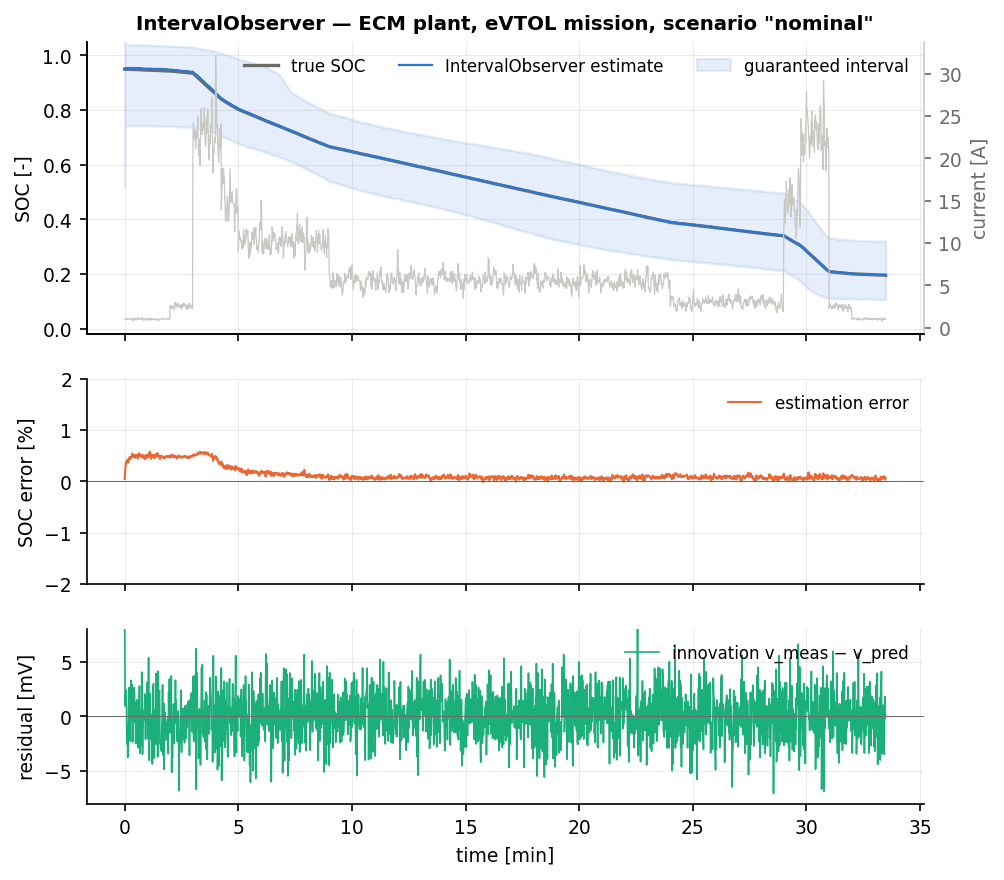
\includegraphics[width=\textwidth]{figures/cell_IntervalObserver_nominal.png}
\caption{IntervalObserver on the nominal eVTOL mission: true and estimated SOC (top), estimation error with the $\pm 2\sigma$ band when available (middle), voltage residual (bottom).}
\end{figure}
\begin{figure}[H]\centering
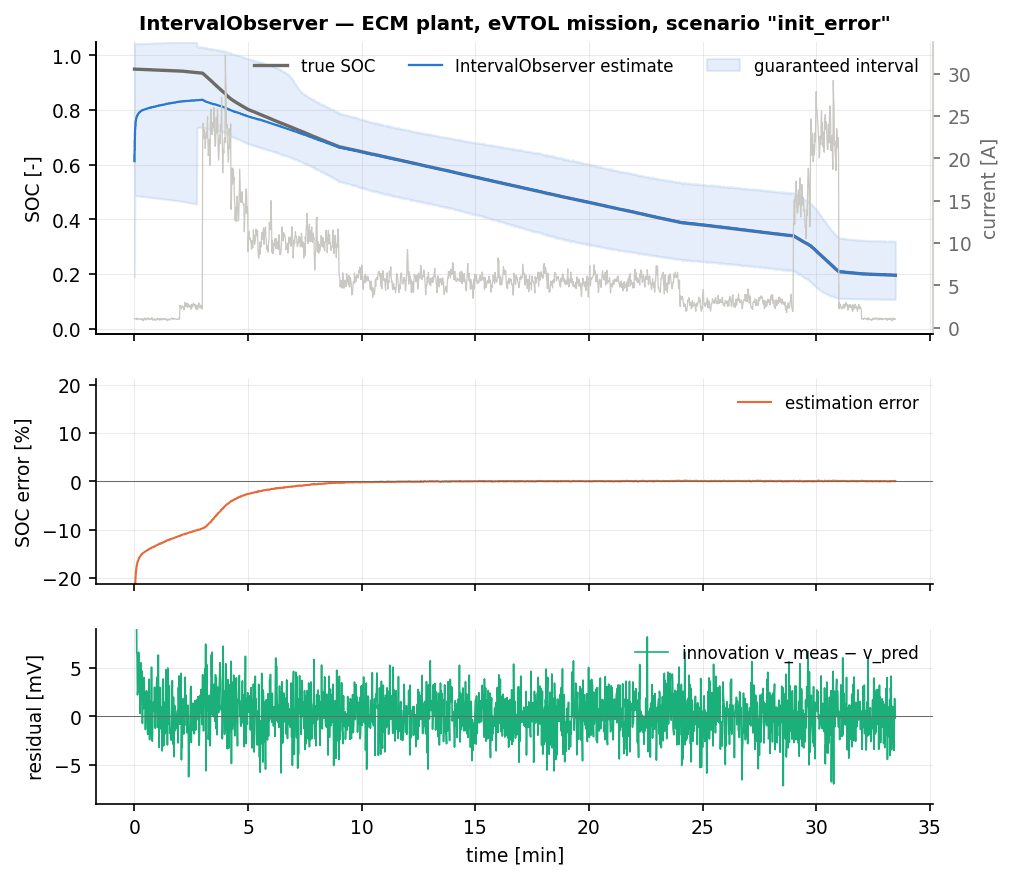
\includegraphics[width=\textwidth]{figures/cell_IntervalObserver_init_error.png}
\caption{IntervalObserver with a 35\,\% initial SOC error.}
\end{figure}

The headline metric is \texttt{bound\_violation}, the fraction of samples at which the true SOC
lies outside $[\soc_{\mathrm{lo}},\soc_{\mathrm{hi}}]$.  It is \textbf{exactly zero in all twelve
scenarios}, including \texttt{outliers} ($5\,\%$ of samples corrupted by $\pm50$\,mV),
\texttt{sensor\_dropout} (15\,s of stuck voltage), \texttt{param\_mismatch} ($-30\,\%$ on $R_0$),
\texttt{aged\_cell} ($-15\,\%$ capacity), \texttt{preisach} (structurally wrong hysteresis) and
\texttt{combined} (four simultaneous faults).  That is the property the method exists to provide,
and it is the only estimator in this study that provides it.

The price is the width: $0.274$ SOC on \texttt{nominal}, $0.252$ on \texttt{hot}, $0.368$ on
\texttt{cold} and $0.318$ on \texttt{combined}.  Decomposing \eqref{eq:io-width} for the nominal
case: $2\bar{v}/C_{\soc} = 2\times0.098/0.94 = 0.209$ from the measurement budget,
$\approx0.04$ from the RC widths, $\approx0.02$ from the SOC padding.  The measurement budget
dominates, and within it the $\pm50$\,mV outlier allowance dominates: a budget that excluded
outliers would give a width near $0.05$ but would then be violated in the \texttt{outliers}
scenario.  The \texttt{cold} case is wider because the RC time constants stretch by a factor of
three, so the open-loop growth of $w_{v_2}$ before the correction acts is larger.

As a point estimator the observer is now exactly as accurate as the \texttt{SSKF} it embeds
(\Cref{sec:io-point}): $\mathrm{rmse}_{ss} = 0.0008$ on \texttt{nominal}, $0.0031$ on
\texttt{cold}, $0.0203$ on \texttt{combined}, $0.0061$ and $0.0335$ on the single-particle plant's
\texttt{nominal} and \texttt{cold}, with the projection \eqref{eq:io-point} almost never binding.
The comparison with the midpoint is the point of the exercise: the midpoint gives $0.0110$,
$0.0196$, $0.0242$, $0.0238$ and $0.0600$ on the same five columns, between $1.2$ and $14$ times
worse, and on the SPM \texttt{nominal} column it is the only number in this family that fails the
$2\,\%$ acceptance threshold.  The bounds are unchanged by the substitution --- the violation count
is still zero and the mean widths are identical to three digits --- so this is a free improvement
of the reported estimate, not a loosening of the guarantee.

The \texttt{init\_error} column converges in $334$\,s with zero violations.

\section{Summary}
Use an interval observer when the deliverable is a guarantee rather than an estimate --- reserve
energy, a certification margin, a fault-detection threshold.  On this benchmark it encloses the
true SOC at every one of $240\,000$ samples across twelve fault scenarios, which no
covariance-based method can claim, at a run-time cost below the EKF's.  Exploit the cooperativity
of the plant, correct a single state, and neutralise the columns of $\mC$ whose sign blocks
monotonicity by widening with their known interval.  Budget the uncertainties honestly and expect
the width to be dominated by the measurement bound through $2\bar{v}/(\partial\ocv/\partial\soc)$;
narrowing that bound, not tuning the gain, is the way to a tighter interval.  Do not use the
midpoint as a point estimate when accuracy matters --- run a Luenberger or unknown-input observer
alongside it --- or, as here, embed one and project its output onto the interval, which costs
nothing and keeps the two answers consistent with each other.

